\documentclass[fontsize = 12pt]{scrartcl}

% Encoding of documents
	\usepackage[utf8]{inputenc}
	\inputencoding{utf8}
	\usepackage[T1]{fontenc}

% Silbensetzung und Automatisch Anpassung der Sprache in generierten Inhalten
	\usepackage[ngerman]{babel}

% Mathematical character set 
    \usepackage{amsmath,amssymb, amsfonts, bm}
	%\usepackage{amsmath,amssymb, amstext, amsfonts}
	\usepackage{dsfont}
	%\usepackage{newtxmath}
	\usepackage[makeroom]{cancel}
 	
 	% equation enumeration
 	\numberwithin{equation}{section}
% Hyperef
	\usepackage{hyperref}

% Font
	\usepackage{txfonts} % TimesNewRoman als Shrift des Fließtextes
					     % Helvetica als serifenlose Schrift für Beispielsweise Überschrift 		
    %\usepackage{pxfonts}
	% \usepackage{lmodern}

	%\usepackage{setspace} % zum Einstellen des zeilenabstandes
	%\setstretch{1.00}

	% Tabular and figure caption
	\usepackage[nooneline]{caption} % noonline sorgt dafür das beschriftung linksbündig ist
	%More info:  https://www.namsu.de/Extra/pakete/Caption.html	
    %	\captionsetup[figure]{labelfont=it, textfont=it} % figure captions
	%   \captionsetup[table]{labelfont=bf, textfont=it} % tabular captions


% including pictures
\usepackage{rotating} % Einfügen und rotieren von Bildern und Graphiken
% \usepackage[final]{graphicx} % Einfügen von Bildern
						     % Setze das Optionale Argument zu 'draft' für schnelleres komplilieren
						     % dann werden bilder durch Rahmen ersetzt.
\usepackage{subcaption}
\usepackage{wrapfig}         % bilder im Fließtext

% tabulars
\usepackage{arydshln} % dashed hlines

% tikz
\usepackage{tikz}
\usetikzlibrary{positioning}
\usetikzlibrary{shapes}
\usetikzlibrary{arrows}
\usetikzlibrary{decorations.markings}

\tikzset{
  arrow_outer/.style={-latex, shorten >=5, shorten <=5,  very thick, color = blue!80}, 
  arrow_inner/.style={-latex, shorten >=2, shorten <=2, thick, color = blue!80},
  arrow_start/.style={-latex, shorten >=2, shorten <=2, thick, color = black!80},
  arrow_double/.style={<->, shorten >=2, shorten <=2, very thick, color = black!80},
  arrow_down/.style={->, shorten >=2, shorten <=2, very thick, color = black!80},
  arrow_grid_in/.style={-latex, shorten >=2, shorten <=2, ultra thick, color = black!100},
  arrow_grid_out/.style={-latex, shorten >=2, shorten <=2, ultra thick, color = black!50},
  grid_point/.style={circle, draw, color=black!100, fill=black!100, minimum size = 8pt, inner sep = 0},
  small_grid_point/.style={circle, draw, color=black!100, fill=black!100, minimum size = 4pt, inner sep = 0},
  small_grid_point_right/.style={circle, draw, color=red!80, fill=red!80, minimum size = 4pt, inner sep = 0}
  ,
  small_grid_point_left/.style={circle, draw, color=blue!80, fill=blue!80, minimum size = 4pt, inner sep = 0}}
% arrow_corner/.style={thick, color = blue!80, decoration={markings, mark=at position 0.5 with{\arrow{latex}}}, postaction={decorate}}

% Utils
\usepackage{placeins}

% pdf einbinden
\usepackage{pdfpages}

% Makro-commands
\newcommand{\corr}[1]{\left\langle #1 \right\rangle}
\newcommand{\Sp}[1]{\mathrm{Sp}\left( #1 \right)}
\renewcommand{\exp}[1]{\mathrm{exp}\left( #1 \right)}
%\renewcommand{\cos}[1]{\mathrm{cos}\left( #1 \right)}
%\renewcommand{\sin}[1]{\mathrm{sin}\left( #1 \right)}
%\renewcommand{\sinh}[1]{\mathrm{sinh}\left( #1 \right)}
%\renewcommand{\tanh}[1]{\mathrm{tanh}\left( #1 \right)}
\newcommand{\atanh}[1]{\mathrm{atanh}\left( #1 \right)}
\newcommand{\sign}[1]{\mathrm{sign}\left( #1 \right)}
\renewcommand{\det}[1]{\mathrm{det}\left( #1 \right)}
\newcommand{\pf}[1]{\mathrm{pf}\left( #1 \right)}
\renewcommand{\ln}[1]{\mathrm{ln}\left( #1 \right)}
\renewcommand{\d}[0]{\mathrm{d}}
\newcommand{\tlim}{ \underset{V,N \to \infty}{\text{lim}^{*}}}

% Umgebungs-commands
\usepackage{mdframed}
\newmdenv[backgroundcolor=black!5, skipabove=12pt, linecolor=white, innerbottommargin = 10pt,
frametitlerule=true, frametitlerulecolor=black, frametitlebackgroundcolor=black!10, frametitlerulewidth=0pt]{grayframe}

\newmdenv[backgroundcolor=black!0, skipabove=12pt, linecolor=white, innerbottommargin = 10pt,
frametitlerule=true, frametitlerulecolor=black, frametitlebackgroundcolor=black!0, frametitlerulewidth=0pt]{whiteframe}

%%%%%%%%%%%%%%%%%%%%%%%%%%%%%%%%%%%%%%%%%%%%%%%%%%%%%%%%%%%%%%%%%%%%%%%%%%%%%%
%%%%%%%%%%%%%%%%%%%%%%%%%%%%%%%%%%%%%%%%%%%%%%%%%%%%%%%%%%%%%%%%%%%%%%%%%%%%%%
\begin{document}

%\title{Analytische Berechnung der spontanen Magnetisierung von isotropen homogenen Ising Ferromagneten unter der Verwendung von Graßmann Zahlen}
% \subtitle{Bachelor Thesis}
%\author{Joachim Pomper}
%\date{22. September 2020}

%\maketitle
%\thispagestyle{empty}

%\newpage

\begin{titlepage}
    \begin{center}
        \vspace*{1cm}
            
        \LARGE
        \textbf{Analytische Berechnung der spontanen Magnetisierung von isotropen homogenen Ising Ferromagneten unter der Verwendung von Graßmann Zahlen}
            
        \vspace{1.5cm}    
        
        \large   
        Eingereicht von:\\
        \vspace{0.3cm}
        \textbf{Joachim Pomper} \\
        \vspace{1.5cm}
        \text{September 2020}\\
        
        \vspace{1.5cm}
        Betreut von:\\
        \vspace{0.3cm}
        Univ.-Prof. Dipl.-Phys. Dr.rer.nat. Wolfgang von der Linden\\
        
        \vfill
            
        Bachelorarbeit
            
        \vspace{0.8cm}
            
        % \includegraphics[width=0.4\textwidth]{university}
            
        \Large
        Technische Universität Graz\\
        %Universität Graz \\
            
    \end{center}
\end{titlepage}

%%%%%%%%%%%%%%%%%%%%%%%%%%%%%%%%%%%%%%%%%%%%%%%%%%%%%%%%%%%%%%%%%%%%%%%%%%%%%%%
\thispagestyle{plain}
\thispagestyle{empty}
\begin{center}
    \Large
    \textbf{Analytische Berechnung der spontanen Magnetisierung von isotropen homogenen Ising Ferromagneten unter der Verwendung von Graßmann Zahlen}
        
    \vspace{0.4cm}
    \large
        
    \vspace{0.4cm}
    \textbf{Joachim Pomper}
       
    \vspace{0.9cm}
    \Large
    \textbf{Abstract}
\end{center}


\noindent Ziel dieser Arbeit ist die Angabe einer möglichst eleganten Herleitung für die exakte Formel der spontanen Magnetisierung des 2d Ising-Modells in Abhängigkeit von der Temperatur, welche erstmals von Lars Onsager aufgestellt wurde. Dies wird bewerkstelligt indem das graphisch-kombinatorische Problem, welches bei der Beschreibung der Zustandssumme und der Magnetisierung auftritt, mithilfe von Graßmann-Zahlen in ein handhabbares algebraisches Problem übersetzt wird. Mathematische Theoreme wie der starke Szegö Grenzwertsatz dienen zudem als praktische Werkzeuge um Grenzübergänge im Thermodynamischen Limes elegant zu behandeln. Die Arbeit beschränkt sich dabei auf ein homogenes isotropes zweidimensionales Ising-Gitter mit periodischen Randbedingungen. Die Ideen zu dieser Herleitung gehen auf die Arbeiten von Stuart Samuel, Elliot W.Montroll, Renfrey B. Potts und John C. Ward zurück. 

\newpage
%%%%%%%%%%%%%%%%%%%%%%%%%%%%%%%%%%%%%%%%%%%%%%%%%%%%%%%%%%%%%%%%%%%%%%%%%%%%%%%
\thispagestyle{empty}
\tableofcontents
\thispagestyle{empty}

\newpage

%%%%%%%%%%%%%%%%%%%%%%%%%%%%%%%%%%%%%%%%%%%%%%%%%%%%%%%%%%%%%%%%%%%%%%%%%%%%%%%
\setcounter{page}{1}

\section{Einleitung} \label{sec: introduction}
    Das Ising-Modell war das erste, nichttriviale Modell eines Ferromagneten und wurde erstmals von seinem Namensgeber Ernst Ising im Rahmen seiner Doktorarbeit 1925 genauer untersucht. Wolfgang Nolting beschreibt die heutige Rolle des Insing-Modells in seinem Lehrbuch wie folgt:
\begin{quote}
``Es hat sich vielmehr zum allgemeinen Demonstatrionsmodell der Statistischen Physik entwickelt. Als das wohl einfachste mikroskopische Modell, das einen Phasenübergang zweiter Ordnung für d $\geq2$ vollzieht, steht es im Mittelpunkt vieler Überlegungen und Untersuchungen der Theorie der Phasenübergänge und kritischen Phänomene.'' \cite{StatPhys_Nolting_K4}
\end{quote}
Bei seinen damaligen Untersuchungen konnte Ising nur das eindimensionale Modell exakt lösen. Für das zweidimensionale Modell legte der norwegische Physiker Lars Onsager erstmals 1944 eine exakte Lösung vor und Aussagen über das dreidimensionale Modell sind bis heute nur numerisch zugänglich.
Im Jahre 1948 publizierte Onsager zudem die in \eqref{eq: expected Magnetisation} angegebene, exakte Formel für die Temperaturabhängigkeit der spontane Magnetisierung des zweidimensionale Ising-Modells, ohne aber seine Herleitung zu veröffentlichen. Erst vier Jahre später, in 1952, gelang es dem Physiker Chen Ning Yang die Formel ebenfalls abzuleiten. Seine Herleitung gilt allerdings als ausgesprochen kompliziert \cite{Montroll_Potts_Ward}.\\
\begin{equation} \label{eq: expected Magnetisation}
\mathcal{M}_S = \left\{ \begin{array}{cr} \mathcal{M}_0\left(1-\frac{1}{\sinh(\frac{2J}{k_B\,T})^4}\right)^{\frac{1}{8}} & \text{für } T < T_c \\ 0 &\text{für } T > T_c   \end{array} \right.
\end{equation}
\begin{quote}
\small
$\mathcal{M}_0$ beschreibt dabei eine Sättigungs-Magentisierung für $T = 0\,\mathrm{K}$ und $J$ ist eine Kopplungskonsante, genannt Austauschintegral, welche die Wechselwirkung zwischen den Spins der Gitteratome beschreibt. Eine ausführlichere Beschreibung des Modells findet sich in Abschnitt \ref{sec: fundamentals}. 
\end{quote}

\noindent 
Die exakte Lösung eines Statistischen Modells ist insofern wichtig, da sie tiefere Einsichten in das Modell liefert und es als Test-Modell für numerische Näherungsmethoden befähigt, mithilfe derer dann nicht exakt lösbare Modelle untersuchte werden können.\\
Das Ziel dieser Arbeit ist nun die Angabe einer möglichst einfachen Herleitung des exakten Ausdrucks für die spontanen Magnetisierung des zweidimensionalen Ising-Modells. Die Koppelung $J$ wird für die Arbeit als homogen Isotrop angenommen und es werden periodische Randbedingungen festgelegt. Die Idee für diesen einfacheren Zugang geht schließlich auf die Arbeiten von Stuart Samuels zurück, der 1980 das Ising-Modell mithilfe von Graßmann-Zahlen beschrieb und zeigte, dass sich so die auftauchenden Probleme statistischer oder graphischer Natur auf einfach handhabbare algebraische Ausdrücke abbilden lassen \cite{StuartSamuel1} \cite{StuartSamuel2}. Zudem bedient sich der hier dargestellte Beweis einer Idee aus dem Paper \cite{Montroll_Potts_Ward} von Elliot W.Montroll, Renfrey B. Potts und John C.Ward, welche das Ising-Modell mithilfe von Pfaffschen Determinanten 1962 untersuchten und denen es gelang die Spin-Spin-Korrelation für zwei beliebig weit entfernte Spins auf elegante Weise mit dem starken Szegö Grenzwertsatz zu berechnen. 
% Die hier angewandten Methoden sind zudem nicht allein auf das Ising-Modell beschränkt, siehe hierzu \cite{StuartSamuel1}.   

\noindent Der Hauptteil der Arbeit gliedert sich in fünf Abschnitte. Die ersten zwei machen dabei circa ein Drittel der Arbeit aus und stellen die nötigen Grundlagen bereit. In Abschnitt \ref{sec: fundamentals} finden sich die physikalischen Grundlagen. Hier wird das Ising-Modell genauer beschrieben, die notwendigen Begriffe aus der Statistischen Physik erklärt und der in der Arbeit zentrale Begriff der spontanen Magnetisierung eingeführt, sowie der Zusammenhang zur Spin-Spin-Korrelation hergestellt. In Abschnitt \ref{sec: grassmann} finden sich die mathematischen Grundlagen. Es wird die notwendige Theorie zu Graßmann-Zahlen, Graßmann-Algebra und Pfaffschen Determinanten aufbereitet. Für den mathematisch interessierten Leser finden sich im Anhang noch ein paar Beweise zu den allgemein bekannte Eigenschaften Pfaffscher Determinanten, welche ausschließlich im Rahmen der Graßmann-Zahlen geführt werden. Im Gegensatz zu Standartbeweisen, benötigen diese keine Vorwissen über die Spektraleigenschaften antisymmetrischer Matrizen. \\
In Abschnitt \ref{sec: reformulation} wird die Berechnung der Zustandssumme des Ising-Modells als Problem des Zählens von geeigneten Graphen auf dem rechteckigen Gitter formuliert und dann mithilfe der Graßmann-Zahlen auf ein algebraisches Problem abgebildet. Zudem wird, über die Hochtemperatur-Darstellung des Ising-Modells, ein Ausdruck für die Spin-Spin-Korrelation abgeleitet, welcher sich als modifizierte Zustandssumme interpretieren lässt und somit das Problem der Magnetisierung auf die zuvor erwähnte algebraische Darstellung der Zustandssumme zurückführt. Abschließend wird noch eine diskrete Fouriertransformation der Graßmann-Zahlen auf dem Ising-Gitter besprochen, welche die Lösung des algebraische Problems stark vereinfacht.\\
Das letzte Drittel der Arbeit machen die Abschnitte \ref{sec: calcC} und \ref{sec: calcM} aus. In Ersterem wird über den algebraischen Ausdruck für die Zustandssumme die Spin-Spin-Korrelation berechnet und der Übergang in den Thermodynamischen Limes vollzogen. Dieser Abschnitt ist der wohl technischste Teil der Arbeit. Hierbei wird insbesondere versucht die Definition der Pfaffschen Determinante in den Vordergrund zu rücken, anstatt diese mithilfe der Relation $\pf{\bm{A}}^2 = \det{\bm{A}}$ auszuwerten. Dieser Zugang erweist sich als elegant und verhindert zudem Vorzeichenprobleme. 
In Abschnitt \ref{sec: calcM} wird letztlich die Magnetisierung über die Korrelation zweier beliebig weit entfernter Spins berechnet. Um den hier benötigten Grenzübergang elegant zu vollziehen kommt der starke Grenzwertsatz von Szegö zum Einsatz. Anhand der Magnetisierung wird das kritische Verhalten und der Phasenübergang des zweidimensionale Ising-Gitters identifiziert, sowie die kritische Temperatur $T_C$ bestimmt.\\
In Abschnitt \ref{sec: conclusio} findet sich dann eine abschließende Analyse des Beweises sowie ein Diskussion weiterer Anwendungsmöglichkeiten für die hier verwendeten Methoden.

\subsection{Bemerkung zur Notation}
In der Arbeit werden Vektoren $\bm{\eta}$ und Matrizen $\bm{A}$ jeweils in ``Boldface''  geschrieben. Die Komponenten werden dann mit dem selben Buchstaben und einem tiefgestellten Index bezeichnet, zum Beispiel $A_{ij}$. Jedoch sind nicht alle indizierten Größen Einträge eines Vektors oder einer Matrix, wie zum Beispiel die klassischen Zufallsvariablen $\sigma_i$.
Lineare und billineare Abbildungen werden immer mit einem Großbuchstaben bezeichnet und die zugehörige Darstellende Matrix wird dem selben Buchsatben in ``Boldface'' notiertet. Speziell Permutation werden immer mit $P$ und die zugehörige Permutationsmatrix mit $\bm{P}$ bezeichnet. 


\section{Grundlagen} \label{sec: fundamentals}
    \subsection{Ferromagnetisches Ising-Modell} \label{sec: Ferromagnetisches Ising-Modell}

Dem Ising-Modell liegt die Vorstellung eines endlichen Gitters zugrunde, auf dessen Gitterpunkten permanente magnetische Momente $\mu_i$ lokalisiert sind. Diese sind alle entlang der selben Achse ausgerichtet, die Orientierung ist jedoch zufällig. Dies ist zum Beispiel ein sehr stark vereinfachtes Modell für einen magnetischen Isolator. Es kann als halbwegs realistisches Modell betrachtet werden, falls das Material eine stark uniaxiale Symmetrie aufweist, da dann eine Richtung für die magnetischen Momente im Material ausgezeichnet ist \cite{StatPhys_Nolting_K4}. Die magnetischen Momente können dabei zum Beispiel von nicht vollbesetzten Hüllen der, an den Gitterplätzen lokalisierten, Atomen eines Kristalls herrühren. In Anlehnung daran werden die magnetische Momente über $\mu_i = \mu \sigma_i$  mit Spin-Variablen $\sigma_i \in \{-1, 1\}$ in Verbindung gebracht, welche als klassische Zufalls-Variablen mit zwei möglichen Einstellungen betrachtet werden. Das als Ising-Modell bekannte System wird dann durch die in \eqref{H_ising_general} angegebene Hamiltonfunktion beschrieben. Betrachtet man ein Gitter mit $N$ Gitterpunkten, so gibt es insgesamt $2^N$ verschieden Konfigurationen welche die Gesamtheit aller Spin-Variablen einnehmen kann. Als klassische Beschreibung, eines eigentlich quantenmechanischen Systems, ist die Hamiltonfunktion diskret und kann höchstens $2^N$ verschiedene Werte annehmen. 
\begin{equation} \label{H_ising_general}
H_{Ising}(\sigma_1, \dots, \sigma_N) = - \sum_{i=1}^N \sum_{j=1}^N J_{i,j} \,\sigma_i \sigma_j \;- \mu H_0 \sum_{i} \sigma_i 
\end{equation}
\noindent Die Größen $J_{i,j}$ werden als Austausch-Integrale bezeichnet. Sie beschreiben den Energieanteil, der aus der gegenseitigen Wechselwirkungen des i-ten und j-ten magnetischen Moments resultiert. Zu dieser Austauschenergie tragen im allgemeinen primär quantenmechanische Effekte bei, welche aus dem Zusammenspiel von Orts- und Spin-Wellenfunktion der Elektronen resultieren. Die erste Summe in \eqref{H_ising_general} beschreibt somit die mit der Spin-Spin-Wechselwirkung in Verbindung gebrachten Energieanteil. Ist $J_{i,j}$ positiv, so führt eine parallele Spinausrichtung an den Gitterpunkten $\bm{x}_i$ und $\bm{x}_j$ zu einer Absenkung der Gesamtenergie und eine antiparallele Spinausrichtung zu einer Erhöhung. Ist $J_{i,j}$ negativ, so verhält es sich genau umgekehrt. Wechselwirkungen von magnetischen Momenten mit sich selbst sollen ausgeschlossen werden, also $\forall i : J_{i,i} = 0$. \\
\noindent Die zweite Summe in \eqref{H_ising_general} beschreibt den Anteil der Energie, welcher durch Anlegen eines externen Magnetfeldes $H_0$ an das Modell-System entsteht.
Für eine detaillierte Herleitung des quantenmechanischen Ising Hamiltonopertors und eine ausführlichere Beschreibung siehe auch \cite{MarxGross2014}.\\

\noindent Für den Rest der Arbeit sollen weitere Vereinfachungen vereinbart werden:
\begin{itemize}
\item[i)] Isotropie und Homogenität des Modells, d.h. $ \forall i\neq j : J_{i,j} = J_{j,i} = J_i = J $
\item[ii)] Nur nächste Nachbar Wechselwirkung, d.h. $\forall i,j : J_{i,j} = 0$ für $\vert i-j \vert > 1$
\item[iii)] Kein externes Magnetfeld, d.h. $H_0 = 0$
\end{itemize}

\noindent Zudem beschränkt sich die Arbeit auf ein zweidimensionales Gitter, welches o.B.d.A in der x-y-Ebene liegen soll. Die Einstellungen der Spins kann man sich dann als Ausrichtung der magnetischen Momente entlang der z-Achse vorstellen. Zudem soll $J > 0$ gelten, um überhaupt eine spontane Magnetisierung erwarten zu können. Ein solches Ising-System, bei dem alle Austausch-Integrale nicht negativ sind, bezeichnet man auch als ferromagnetisch. Die Hamiltonfunktion, welche das System für ein quadratisches Gitter mit Seitenlänge $2M+1$ und somit $N = (2M+1)^2$ Gitterpunkten beschreibt, ist im Folgenden angegeben.

\begin{grayframe}[frametitle = {2d Ising-Modell ohne externes Magnetfeld}]
\begin{align} 
H(\sigma_1, \dots, \sigma_N) &= - J  \sum_{(i,j)} \sigma_i \sigma_j \label{H_ising_2d}\\
  &= - J \sum_{x = -M}^M \sum_{y = -M}^M \sigma_{x, y} \sigma_{x+1, y} + \sigma_{x, y} \sigma_{x,y+1} \label{H_ising_2d_exp} 
\end{align}
\end{grayframe}

\noindent Die Summation in \eqref{H_ising_2d} läuft dabei über alle $2N$ Paare nächster Nachbarn auf dem Gitter. Diese Notation soll für die gesamte Arbeit vereinbart werden.

\begin{equation}
\sum_{(i,j)} \;\text{bzw.}\; \prod_{(i,j)} \iff  \begin{array}{ll} \text{Summe bzw. Produkt über alle Paare} \\ \text{nächster Nachbarn auf dem Gitter} \end{array}
\end{equation}

\noindent Im folgenden wird das Gitter auf zwei unterschiedliche Weisen beschrieben. Einerseits wird das Gitters über eine geeignete Nummerierung der Gitterpunkte und der Angabe des Indexes $j$ beschrieben. Dies wird zum Beispiel bei der Beschreibung nächster Nachbar Paare auf dem Gitter, siehe \eqref{H_ising_2d}, benutzt. Die Nummerierung der Gitterpunkte ist vorerst beliebig, wird aber zu einem späteren Zeitpunkt genauer festgelegt werden. Andererseits wird zur Beschreibung des Gitteres eine explizite Angabe der Koordinaten $\bm{x} = (x,y)$ der Gitterpunkte in der Ebene, wie in \eqref{H_ising_2d_exp}, benutzt. Insbesondere gehen diese beiden Arten der Beschreibung durch die Zuordnung $j \rightarrow \bm{x}_j$ bzw. $\sigma_j = \sigma_{\bm{x}_j}$ fließend ineinander über. Davon wird in der Arbeit mehrmals Gebrauch gemacht werden. 
Die Darstellung in \eqref{H_ising_2d_exp} wirft letztlich die Frage nach den Randbedingungen auf. Es werden periodische Randbedingungen gemäß \eqref{eq: Periodische Randbedingungen} festgelegt. 

\begin{equation} \label{eq: Periodische Randbedingungen}
\begin{aligned} 
\forall y & : \sigma_{M+1, y} =  \sigma_{-M, y} \\
\forall x & : \sigma_{x, M+1} =  \sigma_{x, -M}
\end{aligned}
\end{equation}

\subsection{Elemente der Statistischen Mechanik}

Das im vorherigen Abschnitt beschriebene Ising-Gitter dient nun als statistisches Assemble von N Teilchen, beschrieben durch die Hamiltonfunktion \eqref{H_ising_2d}. Wir gehen davon aus, dass das System in thermischen Kontakt mit einem Wärmebad konstanter Temperatur $T$ steht. Zudem gilt dass sowohl die Ausdehnung $V$, als auch die an Anzahl N der an den Gitterplätzen lokalisierten Momente, konstant sind für jedes Ising-Gitter. Das Assemble kann aus Sicht der statistischen Physik somit als sogenannte kanonische Gesamtheit beschrieben werden. Die Berechnung vieler Größen solcher Systeme können durch die Berechnung der Zustandssumme $Z$ und Erwartungswerte bzw. Korrelationen $\corr{.}$ berechnet werden. Die Zustandssumme ist dabei gemäß

\begin{equation} \label{def: sp_zustandssumme}
 Z(T,N,V) = \sum_{\{S\}} \mathrm{e}^{-\beta H( S ) } 
\end{equation}
definiert, wobei der Faktor $\beta = \beta\left(T\right) = \frac{1}{k_B T} $ eingeführt wurde, welcher die Einheit einer reziproken Energie hat. $k_B$ ist hierbei die Boltzmann-Konstante. Die Summation erfolgt über die Menge alle möglichen Spinkonfigurationen des Systems, geschrieben als $\{S\} = \{S = (\sigma_1, \sigma_2, \dots,\sigma_N) \,\vert\, \forall\,i : \sigma_i \in \{-1, 1\}\}$. Die Wahrscheinlichkeit, dass eine Konfiguration $S$ eingenommen wird, ist dann durch

\begin{equation} \label{eq: konfigProb}
    P(S) = \frac{1}{Z} \mathrm{e}^{-\beta H( S ) } 
\end{equation}
 gegeben. Die Spin-Spin-Korrelation ist der Erwartungswert für das Produkt zweier Spinvariablen und ist gemäß
 
\begin{equation} \label{def: sp_erwartungswert}
    \corr{\sigma_{p} \sigma_{q}}_{T,N,V} = \frac{1}{Z} \sum_{\{S\}} \mathrm{e}^{-\beta H( S ) }  \sigma_{p}( S ) \sigma_{q}( S )
\end{equation}
 definiert. \cite{StatPhys_Nolting_K2} Um das System mit den Mittelen der Statistischen Physik auf Phasenübergänge untersuchen zu können, muss das Ising-Modell im sogenannten Thermodynamik Limes untersucht werden. Dazu wird eine entsprechende Größe, wie die freie Energie, für ein System endlicher Ausdehnung $V$ und Teilchenzahl $N$ berechnet und anschließend mithilfe des Grenzübergangs \eqref{Thermodynamischer Limes} auf ein unendliches System extrapoliert. 
\begin{equation} \label{Thermodynamischer Limes}
\centering
\begin{tabular}{lccccc}
        &  &                 &    &      $N \longrightarrow \infty$\\
$\tlim$ &  &  $\iff$           &   &      $V \longrightarrow \infty$ \\
        &  &                 &   & $n =  N/V = konst. < \infty$
\end{tabular}
\end{equation}

\noindent Der Übergang in den Thermodynamischen Limes ist notwendig, um  Phasenübergänge erkennen zu können, da diese sich als Diskontinuität, Sigularität oder Nicht-Analytizität eines Thermodynamischen Potenzials, wie der Freien Energie, bemerkbar machen. Für endliche Systeme sind diese Potenziale aber immer analytisch. Für das unendlich große System können nur Größen pro Volumen oder Teilchen sinnvoll betrachtet werden. Die Freie Energie pro Teilchen $f$ lässt sich z.B. als Thermodynamischer Limes der Freien Energien $F_N$ endlicher Systemen mit Teilchenzahl $N$ ausdrücken. $F_N$ wiederum kann mit der Zustandsumme des endlichen Systems berechnet werden. \cite{StatPhys_Nolting_K4} 
\begin{equation} \label{SP_FreieEnergie}
f(T,n = \frac{N}{V}) = \tlim \frac{F_N}{N} = \tlim \frac{-k_B T}{N} \ln Z(T,V,N) 
\end{equation}

\subsection{Spontane Magnetisierung}

Abschließend soll noch die Definition des Begriffs der spontane Magnetisierung besprochen werden. Die Magnetisierung $\mathcal{M}$ eines magnetischen Festkörpers wird normalerweise als das mittlere magnetische Moment pro Volumen definiert. Für ein endliches Ising-Gitter $\Lambda_N$ ergibt sich 
\begin{equation} \label{Classic_Magnatization}
\mathcal{M}(N,T,V,H_0)  = \frac{1}{V}\corr{ \mu \sum_i \sigma_i\;}_{\Lambda_N, H_0} = \frac{\mu N}{V}\corr{\sigma_0}_{\Lambda_N, H_0} = n \mu \corr{\sigma_0}_{\Lambda_N, H_0} 
\end{equation}
als eine anschauliche Definition der Magnetisierung des Ising-Systems. Dabei wurde die, durch die angenommene Homogenität und Periodizität des periodischen Gitters implizierte, Translationsinvarianz der Erwartungswerte benutzt. Die Magnetisierung eines beliebig großen Systems ergibt sich letztlich durch Extrapolation mithilfe des Thermodynamischen Limes. Zur Notation sei gesagt dass $\Lambda_N$ andeuted dass ein endliches System mit $N$ Teilchen betrachtet wird und tiefgestelltes $H_0$ verweist auf die Anwesenheit eines externen Magnetfeldes $H_0 > 0$. Als spontane Magnetisierung $M_S$ wird nun die Magnetisierung eines Festkörpers bei verschwindendem externen Magnetfeld bezeichnet. 
\begin{equation} \label{def: classic_spontaneMagnetisierung}
\mathcal{M}_S(T) = \lim_{H_0 \rightarrow 0} \mathcal{M} = \lim_{H_0 \rightarrow 0} \tlim \mathcal{M}(T,N,V,H_0) =  n \mu \lim_{H_0 \rightarrow 0} \tlim \corr{\sigma_0}_{\Lambda_N, H_0} 
\end{equation}
\noindent Die Definition in \eqref{def: classic_spontaneMagnetisierung} wirft dabei jedoch zwei Probleme für die Berechnung der spontanen  Magnetisierung für das hier untersuchte Ising-System auf:
\begin{itemize}
\item [i)] Die Grenzprozesse in \eqref{def: classic_spontaneMagnetisierung} lassen sich im Allgemeinen nicht vertauschen. Somit kann diese Definition für die spontane Magnetisierung möglicherweise nicht angewandt werden. Für das untersuchte System wurde schließlich $H_0 = 0$ festgelegt. 
\item [ii)] Es konnte bislang keine analytische Berechnung für $\corr{\sigma_0}$ gefunden werden.  (Zumindest ist eine solche dem Autor nicht bekannt). 
\end{itemize}

\noindent Um diese Probleme zu umgehen, soll die spontane Magnetisierung stattdessen über die langreichweitige Spin-Spin-Korrelation \eqref{longrangeCorrelation} gemäß \eqref{spontaneMagnetisierung} definiert werden. 
\begin{grayframe}[frametitle = {Definition der spontanen Magnetisierung}]
\begin{align}
l^* & = \lim_{||\bm{x}_i-\bm{x}_j||_1 \rightarrow \infty} \tlim \sqrt{\corr{\sigma_i\sigma_j}_{\Lambda_N}} \label{longrangeCorrelation} 
% \mathcal{M}_S   & = n \mu l^* \label{spontaneMagnetisierung}
\end{align}
\begin{equation}
\mathcal{M}_S  = n \mu l^* \label{spontaneMagnetisierung}
\end{equation}
\end{grayframe}
\noindent Dass dies tatsächlich eine äquivalente Definition für die spontane Magnetisierung darstellt, wird zum Beispiel in einer Arbeit von Anders Martin-Löf \cite{Anders1969} bewiesen. Das Resultat seiner Arbeit kann dabei wie folgt zusammengefasst werden.
\begin{grayframe}[]
    Der Grenzwert $\tlim \corr{\sigma_i\sigma_j}_{\Lambda_N}$ existiert und für $e^{-2J\beta}<\frac{1}{3}$ folgt dass $ n \mu l^{*} = \mathcal{M}_S$ für das 2D-Ising Gitter, unabhängig von den folgenden Randbedingungen :    \\
    
    \begin{tabular}{cl}
        $+$ & Das Gitter wird von Spins mit konstantem Wert $1$ eingeschlossen\\
        $-$ & Das Gitter wird von Spins mit konstantem Wert $-1$ eingeschlossen\\
        $f$ & Es gilt $J_{i,j} = 0$ für $i > M$ oder $j > M$ (freier Rand)\\
        $t$ & Das Gitter hat die Topologie eines Torus (periodische Randbedingungen) \\
    \end{tabular} \\ 

    \noindent Wobei $\mathcal{M}_S$ in diesem Zusammenhang gemäß \eqref{def: classic_spontaneMagnetisierung} definiert ist.
\end{grayframe}

\noindent Dabei entspricht die letzte Bedingung $t$ der hier verwendeten Randbedingung.







\section{Antikommutierende Variablen und Graßmann Algebra} \label{sec: grassmann}
   \input{Chapter/3_Anticommuting_variables_and_Graßmann_Algebra.tex}

\section{Reformulierung des Ising-Modells} \label{sec: reformulation}
    Dieser Abschnitt bildet den Hauptteil der Arbeit. Es wird sich herausstellen, dass die gesuchte Größe zu Berechnung der Magnetisierung, die Spin-Spin-Korrelation, mithilfe der Zustandssumme $Z$ des Ising-Modells ausgedrücken werden kann. Das zentrale Ziel dieses Abschnitts ist es die Zustandssumme $Z$ als Spur einer geeigneten Gauß-Graßmann-Dichte zu schreiben. Denn dann lassen sich Zustandssumme und Spin-Spin-Korrelation  mit den in Abschnitt \ref{sec: grassmann} erarbeiteten Mitteln berechnen. Um diese Reformulierung zu erreichen wird ein Zwischenschritt benötigt, bei dem das Ising-Modell mit einer sogenannten Hochtemperatur-Darstellung auf ein graphisch kombinatorisches Problem abgebildet wird. Dieses kann dann mithilfe der Graßmann-Variablen behandelt werden. Diese Idee geht auf die Arbeiten von Stuart Samuel zurück \cite{StuartSamuel1} \cite{StuartSamuel2}, welcher in seiner ursprünglichen Arbeit jedoch eine Tieftemperatur-Darstellung verwendete. 

\subsection{Hochtemperatur-Entwicklung} 

 \noindent Zu Beginn soll ein expliziter Ausdruck für die Zustandssumme und die Spin-Spin-Korrelation des Ising-Modells abgeleitet werden. Dazu wird mit der Berechnung des Ausdrucks $\exp{\beta J \sigma_i \, \sigma_j} $ für $i \neq j$ begonnen.
\begin{align}
\exp{\beta J \sigma_i \sigma_j} & = \sum_{k=0}^{\infty} \frac{(\beta J)^{2k}}{(2k)!}(\sigma_i \sigma_j)^{2k} + \sum_{k=0}^{\infty} \frac{(\beta J)^{2k+1}}{(2k+1)!}(\sigma_i \sigma_j)^{2k+1} \nonumber  \\
& = \sum_{k=0}^{\infty} \frac{(\beta J)^{2k}}{(2k)!} + (\sigma_i \sigma_j) \sum_{k=0}^{\infty} \frac{(\beta J)^{2k+1}}{(2k+1)!} \nonumber  \\
& = \cosh(\beta J) + (\sigma_i \sigma_j) \sinh(\beta J) \nonumber  \\
& = \cosh(\beta J) \; (1 +  \tanh(\beta J) \; (\sigma_i \sigma_j)) \label{eq: exp(beta J sig sig)}
\end{align}

\noindent Dabei wurde benutzt dass $(\sigma_i \sigma_j)^{2k} = 1$ und $(\sigma_i \sigma_j)^{2k+1} = (\sigma_i \sigma_j)$ gilt. Durch Einsetzen der Hamiltonfunktion \eqref{H_ising_2d} in die Definition der Zustandssumme \eqref{def: sp_zustandssumme} lässt sich für das Ising-Modell ein expliziter Ausdruck für $Z$ finden. Die Summation erfolgt dabei über die Menge aller möglichen Spin-Konfigurationen $\{S\}$ des Gitters.

\begin{align} 
    Z(T,N,V) 
    &  = \sum_{\{S\}} \exp{\beta J \sum_{(i,j)} \sigma_i \sigma_j } \nonumber \\
    &  = \sum_{\{S\}} \prod_{(i,j)} \exp{\beta J \sigma_i \sigma_j } \nonumber\\
    &  = \cosh(\beta J)^{2N} \sum_{\{S\}} \prod_{(i,j)} (1 +  \tanh(\beta J) \; (\sigma_i \sigma_j)) \nonumber \\
    &  = \cosh(\beta J)^{2N} \sum_{\{S\}} \prod_{(i,j)} (1 +  t \; (\sigma_i \sigma_j))
\end{align}

\noindent Bei dieser Ableitung wurde die Größe $t = \tanh(\beta J)$ eingeführt. Die Potenz $2N$ rührt von der Anzahl der Paare nächster Nachbarn auf dem Gitter her. Siehe dazu auch Abbildung \ref{Abb: grid}.
\begin{figure}[h]
    \centering
    \begin{tikzpicture}[scale = 1.5]
\begin{scope}
    \node[draw = none] at (0,0)   (p0p0) {$\sigma$};
\node[draw = none] at (0,1)   (p0p1) {$\sigma$};
\node[draw = none] at (1,0)   (p1p0) {$\sigma$};
\node[draw = none] at (0,-1)  (p0m1) {$\sigma$};
\node[draw = none] at (-1,0)  (m1p0) {$\sigma$};
\node[draw = none] at (1,-1)  (p1m1) {$\sigma$};
\node[draw = none] at (-1,1)  (m1p1) {$\sigma$};
\node[draw = none] at (-1,-1) (m1m1) {$\sigma$};
\node[draw = none] at (1,1)   (p1p1) {$\sigma$};

\node[draw = none] at (1.7,0)   (p2p0) {};
\node[draw = none] at (1.7,1)   (p2p1) {};
\node[draw = none] at (1,1.7)   (p1p2) {};
\node[draw = none] at (0,1.7)   (p0p2) {};
\node[draw = none] at (-1,1.7)  (m1p2) {};
\node[draw = none] at (-1.7,1)  (m2p1) {};
\node[draw = none] at (-1.7,0)  (m2p0) {};
\node[draw = none] at (-1.7,-1) (m2m1) {};
\node[draw = none] at (-1,-1.7) (m1m2) {};
\node[draw = none] at (0,-1.7)  (p0m2) {};
\node[draw = none] at (1,-1.7)  (p1m2) {};
\node[draw = none] at (1.7,-1)  (p2m1) {};

%% arrows
\draw[arrow_grid_in] (p0p0) -- (p0p1);
\draw[arrow_grid_in] (p0p0) -- (p1p0);

\draw[arrow_grid_in] (p1p0) -- (p1p1);


\draw[arrow_grid_in] (p0p1) -- (p1p1);
\draw[arrow_grid_out] (p0p1) -- (p0p2);

\draw[arrow_grid_out] (p1p1) -- (p1p2);


\draw[arrow_grid_in] (p1m1) -- (p1p0);


\draw[arrow_grid_in] (p0m1) -- (p0p0);
\draw[arrow_grid_in] (p0m1) -- (p1m1);

\draw[arrow_grid_in] (m1m1) -- (m1p0);
\draw[arrow_grid_in] (m1m1) -- (p0m1);

\draw[arrow_grid_in] (m1p0) -- (m1p1);
\draw[arrow_grid_in] (m1p0) -- (p0p0);

\draw[arrow_grid_in] (m1p1) -- (p0p1);
\draw[arrow_grid_out] (m1p1) -- (m1p2);



\draw[arrow_grid_out] (m1m2) -- (m1m1);
\draw[arrow_grid_out] (p0m2) -- (p0m1);
\draw[arrow_grid_out] (p1m2) -- (p1m1);


    \draw[arrow_grid_out] (m2p1) -- (m1p1);
    \draw[arrow_grid_out] (m2p0) -- (m1p0);
    \draw[arrow_grid_out] (m2m1) -- (m1m1);

\end{scope}
\begin{scope}[shift = {(2,0)}]
    \node[draw = none] at (0,0)   (p0p0) {$\sigma$};
\node[draw = none] at (0,1)   (p0p1) {$\sigma$};
\node[draw = none] at (1,0)   (p1p0) {$\sigma$};
\node[draw = none] at (0,-1)  (p0m1) {$\sigma$};
\node[draw = none] at (-1,0)  (m1p0) {$\sigma$};
\node[draw = none] at (1,-1)  (p1m1) {$\sigma$};
\node[draw = none] at (-1,1)  (m1p1) {$\sigma$};
\node[draw = none] at (-1,-1) (m1m1) {$\sigma$};
\node[draw = none] at (1,1)   (p1p1) {$\sigma$};

\node[draw = none] at (1.7,0)   (p2p0) {};
\node[draw = none] at (1.7,1)   (p2p1) {};
\node[draw = none] at (1,1.7)   (p1p2) {};
\node[draw = none] at (0,1.7)   (p0p2) {};
\node[draw = none] at (-1,1.7)  (m1p2) {};
\node[draw = none] at (-1.7,1)  (m2p1) {};
\node[draw = none] at (-1.7,0)  (m2p0) {};
\node[draw = none] at (-1.7,-1) (m2m1) {};
\node[draw = none] at (-1,-1.7) (m1m2) {};
\node[draw = none] at (0,-1.7)  (p0m2) {};
\node[draw = none] at (1,-1.7)  (p1m2) {};
\node[draw = none] at (1.7,-1)  (p2m1) {};

%% arrows
\draw[arrow_grid_in] (p0p0) -- (p0p1);
\draw[arrow_grid_in] (p0p0) -- (p1p0);

\draw[arrow_grid_in] (p1p0) -- (p1p1);


\draw[arrow_grid_in] (p0p1) -- (p1p1);
\draw[arrow_grid_out] (p0p1) -- (p0p2);

\draw[arrow_grid_out] (p1p1) -- (p1p2);


\draw[arrow_grid_in] (p1m1) -- (p1p0);


\draw[arrow_grid_in] (p0m1) -- (p0p0);
\draw[arrow_grid_in] (p0m1) -- (p1m1);

\draw[arrow_grid_in] (m1m1) -- (m1p0);
\draw[arrow_grid_in] (m1m1) -- (p0m1);

\draw[arrow_grid_in] (m1p0) -- (m1p1);
\draw[arrow_grid_in] (m1p0) -- (p0p0);

\draw[arrow_grid_in] (m1p1) -- (p0p1);
\draw[arrow_grid_out] (m1p1) -- (m1p2);



\draw[arrow_grid_out] (m1m2) -- (m1m1);
\draw[arrow_grid_out] (p0m2) -- (p0m1);
\draw[arrow_grid_out] (p1m2) -- (p1m1);


    \node[draw = none, scale = 1] at (-0.34,0.5)   (J) {$J_{i,j}$};
    \node[draw = none, scale = 1] at ( 0.5,-0.28)   (J) {$J_{i,k}$};
    \node[draw = none, scale = 0.8] at (0.1, -0.1)   (J) {$i$};
    \node[draw = none, scale = 0.8] at (1.1, -0.1)   (J) {$k$};
    \node[draw = none, scale = 0.8] at (0.1,  0.9)   (J) {$j$};
    %\node[draw = none, scale = 1] at (-0.25, -0.2)   (J) {$\sigma_i$};
\end{scope}
\begin{scope}[shift = {(4,0)}]
    \node[draw = none] at (0,0)   (p0p0) {$\sigma$};
\node[draw = none] at (0,1)   (p0p1) {$\sigma$};
\node[draw = none] at (1,0)   (p1p0) {$\sigma$};
\node[draw = none] at (0,-1)  (p0m1) {$\sigma$};
\node[draw = none] at (-1,0)  (m1p0) {$\sigma$};
\node[draw = none] at (1,-1)  (p1m1) {$\sigma$};
\node[draw = none] at (-1,1)  (m1p1) {$\sigma$};
\node[draw = none] at (-1,-1) (m1m1) {$\sigma$};
\node[draw = none] at (1,1)   (p1p1) {$\sigma$};

\node[draw = none] at (1.7,0)   (p2p0) {};
\node[draw = none] at (1.7,1)   (p2p1) {};
\node[draw = none] at (1,1.7)   (p1p2) {};
\node[draw = none] at (0,1.7)   (p0p2) {};
\node[draw = none] at (-1,1.7)  (m1p2) {};
\node[draw = none] at (-1.7,1)  (m2p1) {};
\node[draw = none] at (-1.7,0)  (m2p0) {};
\node[draw = none] at (-1.7,-1) (m2m1) {};
\node[draw = none] at (-1,-1.7) (m1m2) {};
\node[draw = none] at (0,-1.7)  (p0m2) {};
\node[draw = none] at (1,-1.7)  (p1m2) {};
\node[draw = none] at (1.7,-1)  (p2m1) {};

%% arrows
\draw[arrow_grid_in] (p0p0) -- (p0p1);
\draw[arrow_grid_in] (p0p0) -- (p1p0);

\draw[arrow_grid_in] (p1p0) -- (p1p1);


\draw[arrow_grid_in] (p0p1) -- (p1p1);
\draw[arrow_grid_out] (p0p1) -- (p0p2);

\draw[arrow_grid_out] (p1p1) -- (p1p2);


\draw[arrow_grid_in] (p1m1) -- (p1p0);


\draw[arrow_grid_in] (p0m1) -- (p0p0);
\draw[arrow_grid_in] (p0m1) -- (p1m1);

\draw[arrow_grid_in] (m1m1) -- (m1p0);
\draw[arrow_grid_in] (m1m1) -- (p0m1);

\draw[arrow_grid_in] (m1p0) -- (m1p1);
\draw[arrow_grid_in] (m1p0) -- (p0p0);

\draw[arrow_grid_in] (m1p1) -- (p0p1);
\draw[arrow_grid_out] (m1p1) -- (m1p2);



\draw[arrow_grid_out] (m1m2) -- (m1m1);
\draw[arrow_grid_out] (p0m2) -- (p0m1);
\draw[arrow_grid_out] (p1m2) -- (p1m1);


    \draw[arrow_grid_out] (p1p0) -- (p2p0);
    \draw[arrow_grid_out] (p1p1) -- (p2p1);
    \draw[arrow_grid_out] (p1m1) -- (p2m1);
\end{scope}

\end{tikzpicture}
    \caption{Darstellung der paarweisen Austauschwechselwirkungen $J_{i,j}$. Unter der Berücksichtigung periodischer Randbedingungen (hellgraue Pfeile) gibt es genau zwei Austasuchintegrale pro Gitterpunkt.}  \label{Abb: grid}
\end{figure}

\noindent Analog lässt sich ein expliziter Ausdruck für die Spin-Spin-Korrelation des Ising-Modells berechnen \cite{StatPhys_Nolting_K4}.
\begin{align} 
    \corr{\sigma_{p} \sigma_{q} }_{T,N,V}  
    % &= \frac{1}{Z} \sum_{\{S\}} e^{-\beta H( S ) }  \sigma_{p}( S ) \sigma_{q}( S ) \nonumber \\
    & = \frac{1}{Z} \sum_{\{S\}} \exp{\beta J \sum_{(i,j)} \sigma_i \sigma_j } \sigma_{p} \sigma_{q} \nonumber\\
    & = \frac{1}{Z} \cosh(\beta J)^{2N} \sum_{\{S\}} \left(\prod_{(i,j)} (1 +  t \; (\sigma_i \sigma_j) )\right) \sigma_{q} \sigma_{q} 
\end{align}

\noindent Die hier abgeleiteten Ausdrücke sind in  \eqref{Ising_Zustandssumme} und \eqref{Ising_SpinSpinCorrelation} noch einmal zusammengefasst. Der Name ``Hochtemperatur-Entwiklung'' rührt daher, dass die Exponentialfunktion um $|\beta J \sigma_i \sigma_j| = \frac{J}{k_B\,T}\ \approx 0 $ entwickelt wird. Da aber die Potenzreihe der Exponentialfunktion auf ganz $\mathbb R$ analytisch ist, ist diese Darstellung der Zustandssumme tatsächlich auch für niedere Temperaturen exakt. 

\begin{grayframe}[frametitle = {Zustandssumme und Spin-Spin-Korrelation für 2d Ising-Modell \cite{StatPhys_Nolting_K4}}]
\begin{align}
 Z(T,N,V)  
  & = \cosh(\beta J)^{2N} \sum_{\{S\}} \prod_{(i,j)} (1 +  t \; (\sigma_i \sigma_j)) \label{Ising_Zustandssumme} \\
\corr{\sigma_{p} \sigma_{q} }_{T,N,V} 
  & = \frac{1}{Z} \cosh(\beta J)^{2N} \sum_{\{S\}} \left(\prod_{(i,j)} (1 +  t \; (\sigma_i \sigma_j) )\right) \sigma_{q} \sigma_{q} \label{Ising_SpinSpinCorrelation}
\end{align}
\centering
\noindent Die Summation läuft dabei über alle $2^N$ Spinkonfigurationen des Gitters
$$\{S\} = \{S = (\sigma_1, \sigma_2, \dots,\sigma_N) \,\vert\, \forall\,i : \sigma_i \in \{-1, 1\}\}$$
\noindent Dimensionloser Parameter $t$
$$ t = \tanh(\frac{J}{k_B T})\in [0,1]$$
\end{grayframe}

\subsection{Korrelation als Zustandssumme auf defektem Gitter} 

Es soll nun eine Verbindung zwischen der Spin-Spin-Korrelation und der Zustandssumme des Ising-Modells hergestellt werden. 

\noindent Man betrachte 2 Punkte $\bm{x}_p$, $\bm{x}_q$ auf dem Gitter. Diese können immer durch eine Strecke auf dem Gitter verbunden werden. Diese Strecke ist nicht eindeutig und soll mit $L_D$ bezeichnet werden. Weiteres soll $D = \{ (i,j) \,|\, i,j \in L_D\ \wedge |i-j| = 1 \}$ die Menge der Paare nächster Nachbarn in $L_D$ sein. $D$ soll als Gitterdefekt bezeichnet werden. Unter Verwendung der Eigenschaft $\sigma_{i}^{2} = 1$ erhält man
\begin{equation} \label{eq: spin_spin_prod}
\sigma_{p} \sigma_{q} = \prod_{\bm{x}_i \in L_D} \sigma_{i}^{2} \,\sigma_{p}\,\sigma_{q} = \prod_{(i,j) \in D} \sigma_{i}\sigma_{j} 
\end{equation}
Mithilfe dieser Relation kann nun die Summe in \eqref{Ising_SpinSpinCorrelation} umgeschrieben werden. 
\begin{align} 
 \sum_{\{S\}} \left(\prod_{(i,j)} (1 +  t \; (\sigma_i \sigma_j))\textbf{ }\sigma_{q} \sigma_{q}\right) 
  & = \sum_{\{S\}} \left(\prod_{(i,j) \notin D } ((1 +  t \; (\sigma_i \sigma_j))\right) \left(\prod_{(i,j) \in D} \sigma_i \sigma_j\right) \nonumber \\
  & = \sum_{\{S\}} \left(\prod_{(i,j) \notin D} ((1 +  t \; (\sigma_i \sigma_j))\right) \left(\prod_{(i,j) \in D} ((1 +  t \; (\sigma_i \sigma_j))\sigma_i \sigma_j \right) \nonumber\\
  & = \sum_{\{S\}} \left(\prod_{(i,j) \notin D} ((1 +  t \; (\sigma_i \sigma_j))\right) \left(\prod_{(i,j) \in D} (((\sigma_i \sigma_j) +  t)\right)  \nonumber\\
  & = t^m \sum_{\{S\}} \left(\prod_{(i,j) \notin D} ((1 +  t \; (\sigma_i \sigma_j))\right) \left(\prod_{(i,j) \in D} (((1 + \frac{1}{t}\sigma_i \sigma_j))\right) \nonumber\\
  &= t^m \sum_{\{S\}} \left(\prod_{(i,j)} (1 + t_{i,j} \; (\sigma_i \sigma_j)) \right) \label{eq: corr_sum}
\end{align}

\noindent Hierbei ist $m = \#D$ die Anzahl der Paare in $D$. Bis auf den Vorfaktor $t^m$ lässt sich in \eqref{eq: corr_sum} die Summe als Zustandssumme des Ising-Modells mit modifiziertem ortsabhängigem $t$ identifizieren.

\begin{grayframe}[frametitle = {Spin Korrelation als Zustandsumme auf defektem Gitter}]
\begin{equation}
\corr{\sigma_{p} \sigma_{q} }_{T,N,V} = \frac{t^m Z_D}{Z}
\end{equation}
\begin{equation} \label{eq: Defekte Zustanssumme}
Z_D = \cosh(\beta J)^{2N} \sum_{\{S\}} \prod_{(i,j)} (1 +  t_{i,j} \; (\sigma_i \sigma_j)) 
\end{equation}
\begin{equation} \nonumber
t_{i,j} = \left\{\begin{array}{ll} t^{-1} & \text{für}\; (i,j)\in D \\
          t & \text{sonst} \end{array} \right.
\end{equation}
\end{grayframe}

\subsection{Graphische Repräsentation der Zustandssumme} \label{sec: GR_Zustandssumme}

Aufgrund von \eqref{eq: Defekte Zustanssumme} muss zur Reformulierung des Ising-Modells ein Ausdruck für die Zustandssumme mit beliebigen $t_{i,j}$ gefunden werden.
Bei der Auswertung des Produkts in \eqref{eq: Defekte Zustanssumme} erhält man eine Summe, bei der die Summanden aus der Entscheidung für $1$ oder $t_{i,j}\,\sigma_i \sigma_j$ in jedem Multiplikanten herrührt. Es handelt sich also um eine Summation über alle Produkte von Spin-Paaren unterschiedlicher Länge $n \in \{0,1,\dots ,2N\}$. 
\begin{align}
\sum_{\{S\}} \prod_{(i,j)} (1 +  t_{i,j} \; (\sigma_i \sigma_j)) 
&= 
\sum_{\{S\}} 1 + \sum_{(i,j)} t_{i,j}\,(\sigma_i \sigma_j) + \sum_{(i,j)}\sum_{(k,l)} t_{i,j}\, t_{k,l}\,(\sigma_i \sigma_j)  (\sigma_k \sigma_l) \dots \nonumber \\
&= \sum_{\{S\}} \, \sum_{\{(i_1,j_1,...,i_n,j_n)\}} t_{i_1,j_1} \cdots t_{i_n,j_n} \, (\sigma_{i_1} \sigma_{j_1})(\sigma_{i_2} \sigma_{i_2}) \cdots (\sigma_{i_n} \sigma_{j_n}) \nonumber
\end{align}

\noindent Aufgrund der Summation über alle Spinkonfigurationen $S$ tragen alle Produkte, in denen zumindest eine Spinvariable $\sigma_k$ in ungerader Anzahl vorkommt, nicht zum Gesamtergebnisse bei. Denn für jede Konfiguration $S = (\sigma_1, \dots, \sigma_k, \dots, \sigma_{2N})$ gibt es genau eine weitere Konfiguration $S' = (\sigma_1, \dots, -\sigma_k, \dots, \sigma_{2N})$, sodass sich diese dann aufheben. Eine Produkt von Isingsspin Paaren, in dem jede Spinvariable in gerader Anzahl vorkommt, hat hingegen immer den Wert 1, unabhängig von der Spinkonfiguration $S$. Durch die Summation über die Spinkonfigurationen entsteht dann ein Vorfaktor $2^N$ für diese Terme.
\begin{figure}[h!]
    \centering
    \begin{tikzpicture}[scale = 1.2]
     \draw[step=1cm,gray, ultra thin] (-3.5,-1.5) grid (4.5,1.5);

\node[grid_point] at (-3,1)   (m3p1) {};
\node[grid_point] at (-3,0)   (m3p0) {};
\node[grid_point] at (-3,-1)  (m3m1) {};

\node[grid_point] at (-2,1)   (m2p1) {};
\node[grid_point] at (-2,0)   (m2p0) {};
\node[grid_point] at (-2,-1)  (m2m1) {};

\node[grid_point] at (-1,1)   (m1p1) {};
\node[grid_point] at (-1,0)   (m1p0) {};
\node[grid_point] at (-1,-1)  (m1m1) {};

\node[grid_point] at (0,1)   (p0p1) {};
\node[grid_point] at (0,0)   (p0p0) {};
\node[grid_point] at (0,-1)  (p0m1) {};

\node[grid_point] at (3,1)   (p3p1) {};
\node[grid_point] at (3,0)   (p3p0) {};
\node[grid_point] at (3,-1)  (p3m1) {};

\node[grid_point] at (2,1)   (p2p1) {};
\node[grid_point] at (2,0)   (p2p0) {};
\node[grid_point] at (2,-1)  (p2m1) {};

\node[grid_point] at (1,1)   (p1p1) {};
\node[grid_point] at (1,0)   (p1p0) {};
\node[grid_point] at (1,-1)  (p1m1) {};

\node[grid_point] at (4,1)   (p4p1) {};
\node[grid_point] at (4,0)   (p4p0) {};
\node[grid_point] at (4,-1)  (p4m1) {};

%% Graph
\draw[-, black!100, very thick] (m3p1) -- (m2p1) ;
\draw[-, black!100, very thick] (m2p1) -- (m1p1) ;
\draw[-, black!100, very thick] (m1p1) -- (m1p0) ;
\draw[-, black!100, very thick] (m1p0) -- (p0p0) ;
\draw[-, black!100, very thick] (p0p0) -- (p0m1) ;
\draw[-, black!100, very thick] (p0m1) -- (m1m1) ;
\draw[-, black!100, very thick] (m1m1) -- (m2m1) ;
\draw[-, black!100, very thick] (m2m1) -- (m3m1) ;
\draw[-, black!100, very thick] (m3m1) -- (m3p0) ;
\draw[-, black!100, very thick] (m3p0) -- (m3p1) ;

\draw[-, black!100, very thick] (p1p1) -- (p2p1) ;
\draw[-, black!100, very thick] (p2p1) -- (p3p1) ;
\draw[-, black!100, very thick] (p3p1) -- (p3p0) ;
\draw[-, black!100, very thick] (p3p0) -- (p4p0) ;
\draw[-, black!100, very thick] (p4p0) -- (p4m1) ;
\draw[-, black!100, very thick] (p4m1) -- (p3m1) ;
\draw[-, black!100, very thick] (p3m1) -- (p3p0) ;
\draw[-, black!100, very thick] (p3p0) -- (p2p0) ;
\draw[-, black!100, very thick] (p2p0) -- (p1p0) ;
\draw[-, black!100, very thick] (p1p0) -- (p1p1) ;

    \end{tikzpicture}
    \caption{Ein möglicher Graph auf dem Gitter mit einer Selbstüberschneidung}
    \label{Abb: erlaubte Graphen}
\end{figure}

\noindent Identifiziert man jedes Spin-Paar als Verbindunsglinie zwischen den zugehörigen Gitterpunkten, so repräsentiert jedes Spin-Paar-Produkt genau einen Graphen $G$ auf dem Gitter. Die Kanten $K_G$ des Graphen entsprechen dann genau den Spin-Paare. Die zugehörigen Gitterpunkte sind die Vertizes $V_G$ des Graphen. Da nur die Produkte beitragen, in denen jede Spin-Variablen in gerader Anzahl vorkommt, schließen an jeden Vertex $0$, $2$ oder $4$ Kanten an. Daher muss ein solcher Graph geschlossen sein. Zudem durchläuft man, wenn man sich in dem Spin-Paar-Produkt von Gitterpunkt zu Gitterpunkt hangelt, jede Kante nur genau einmal, da jedes Spin-Paar nur einmal im Produkt vorkommt. Dabei ist zu beachten, dass ein Graph aus mehreren getrennten sich selbst überschneidenden Schleifen bestehen darf, wie zum Beispiel in Abbildung \ref{Abb: erlaubte Graphen} gezeigt ist. Zudem dürfen die Graphen auch über den periodischen Rand schließen. 
Da das Produkt in \eqref{eq: Defekte Zustanssumme} über alle Paare nächster Nachbarn und damit Spin-Paare geht, werden alle möglichen Graphen, mit diesen Eigenschaften erzeugt. Man kann die Zustandssumme $Z_D$ dann, wie in \eqref{eq: GR_Zustanssumme} also als Summe über alle geeigneten Graphen schreiben. 
Das Gewicht eines Graphen wird durch das Produkt der zu den Kanten gehörigen $t_{i,j}$ bestimmt.  

\begin{grayframe}[frametitle = {Graphische Representation der Summe $Z_D$} ]
\begin{equation} \label{eq: GR_Zustanssumme}
Z_D = 2^N \cosh(\beta J)^{2N} \sum_{\{G\}} \prod_{(i,j)\in K_{G}} t_{i,j}
\end{equation} 
\\
Die Graphen $G = (V_G, K_G)$ besitzen die Eigenschaften: 
\begin{itemize}
\item[i)] Alle Vertices des Graphen liegen auf dem Gitter
\item[ii)] $G$ ist geschlossen (auch über periodischen Rand)
\item[iii)] $G$ kann durchlaufen werden ohne eine Kante zweimal zu nutzen. 
\end{itemize}
\end{grayframe}

\noindent Für den Fall des nicht defekten Gitters wird das Gewicht der Graphen allein durch die Anzahl $N_K(G)$ der Kanten bestimmt.

\begin{equation} \label{eq: GR_pseudo_ustandssumme}
\sum_{\{S\}} \prod_{(i,j)} (1 +  t \; (\sigma_i \sigma_j)) = 2^N \sum_{\{ G\}} t^{N_K(G)}
\end{equation}

\subsection{Graphen ausgedrückt durch Graßmann-Variablen } \label{sec: GraßmanGraphs}

\noindent Im Folgenden bezeichne  $\Lambda$ das Ising-Gitter mit $N$ Gitterpunkten. Für jeden Gitterpunkt $\bm{x}_i$ werden vier Graßmann-Variablen $h_{\bm{x}_i}^o, h_{\bm{x}_i}^x, v_{\bm{x}_i}^o, v_{\bm{x}_i}^x$ eingeführt. 
\begin{figure}[h]
\centering
\begin{tikzpicture}[scale = 0.4]
    \node[draw = none] at (0,0) (center) {$i$} ;
    \node[draw, circle, fill=none, scale = 0.5, very thick] at (-1,0) (center) {} ;
    \node[draw, circle, fill=none, scale = 0.5, very thick] at (0,-1)  {} ;
    \node[draw, cross out, very thick, scale = 0.6] at (1,0)  {} ;
    \node[draw, cross out, very thick, scale = 0.6] at (0,1)  {} ;
    \node[draw=none] at (-2,0)  {$h_{i}^o$} ;
    \node[draw=none] at (0,-2)  {$v_{i}^o$} ;
    \node[draw=none] at (2,0) {$h_{i}^x$} ;
    \node[draw=none] at (0,2) {$v_{i}^x$} ;
\end{tikzpicture}
\caption{Graßmann-Variablen assoziiert mit Gitterpunkt $\bm{x}_i\in\Lambda$}
\label{Abb: graßmanVariableBeiI}
\end{figure}

\noindent Neben der Position am Gitter besitzt jede Variable eine Orientierung, gekennzeichnet mit $h$ für ``Horizontal'' und $v$ für ``Vertikal'' und eine Fluss-Richtung, gekennzeichnet durch $o$ für ``hinein'' und $x$ für ``hinaus''. Variablen wie $h_{i}^x$ und $h_{i}^o$  mit gleicher Orientierung und unterschiedlicher Fluss-Richtung werden als zueinander konjugiert bezeichnet. Die Reihenfolge der Generatoren der so erzeugten Graßmann-Algebra wird in dem Graßmann-Vektor \eqref{def: hv_gv_vektor} beziehungsweise in dem ``Integrationsmaß'' \eqref{def: hv_measure} festgehalten.
\begin{equation} \label{def: hv_gv_vektor}
\bm{\eta} = \left(h_{\bm{x}_1}^o, h_{\bm{x}_1}^x, v_{\bm{x}_1}^o, v_{\bm{x}_1}^x, \dots, h_{\bm{x}_N}^o, h_{\bm{x}_N}^x, v_{\bm{x}_N}^o, v_{\bm{x}_N}^x \right)
\end{equation}
\begin{equation} \label{def: hv_measure}
\mathrm{D}_{h,v} = \prod_{\bm{x}_i \in \Lambda} \d h_{\bm{x}_i}^x\,\d h_{\bm{x}_i}^o\,\d v_{\bm{x}_i}^x\,\d v_{\bm{x}_i}^o \\
\end{equation}

 \noindent Die Nummerierung der Gitterpunkte ist dabei grundsätzlich egal, da Paare von Graßmann-Variablen miteinander kommutieren. Um später aber die darstellenden Matrix bezüglich dem in \eqref{def: hv_gv_vektor} angegeben Vektor jedoch möglichst einfach zu gestalten, soll die Numerierung der Gitterpunkt nun wie in Abb. \ref{Abb: Numerierung} festgelegt werden. Diese Nummerierung besitzt die Eigenschaft, dass ein Verschiebung der Indizierung um $2M(M+1)$ durch eine Punktspiegelung erreicht wird. 
\begin{figure}[h!]
\centering
\begin{tikzpicture}[scale = 1.2]

\begin{scope}[shift = {(-3,0)}]


\node[small_grid_point] at (0,0) (0){}; 

% right grid point
\node[small_grid_point_right] at (0,1)  {}; 
\node[small_grid_point_right] at (0,2) {}; 
\node[small_grid_point_right] at (1,-2) {}; 
\node[small_grid_point_right] at (1,-1) {}; 
\node[small_grid_point_right] at (1,0) (10){}; 
\node[small_grid_point_right] at (1,1) (1) {}; 
\node[small_grid_point_right] at (1,2) {}; 
\node[small_grid_point_right] at (2,-2) {}; 
\node[small_grid_point_right] at (2,-1) (3){}; 
\node[small_grid_point_right] at (2,0) (20){}; 
\node[small_grid_point_right] at (2,1) {}; 
\node[small_grid_point_right] at (2,2) {}; 

%%% left grid
\node[small_grid_point_left] at (0,-1) {}; 
\node[small_grid_point_left] at (0,-2) {}; 
\node[small_grid_point_left] at (-1,-2) {}; 
\node[small_grid_point_left] at (-1,-1) (2){}; 
\node[small_grid_point_left] at (-1,0) {}; 
\node[small_grid_point_left] at (-1,1) {}; 
\node[small_grid_point_left] at (-1,2) {}; 
\node[small_grid_point_left] at (-2,-2) {}; 
\node[small_grid_point_left] at (-2,-1) {}; 
\node[small_grid_point_left] at (-2,0) {}; 
\node[small_grid_point_left] at (-2,1) (4){}; 
\node[small_grid_point_left] at (-2,2) {}; 


\node[draw = none, scale = 1] at (0.3,0.3) {0};
%%% right grid
\node[draw = none, scale = 1] at (0.3,1.3) {1};
\node[draw = none, scale = 1] at (0.3,2.3) {2};
\node[draw = none, scale = 1] at (1.3,-1.7) {3};
\node[draw = none, scale = 1] at (1.3,-0.7) {4};
\node[draw = none, scale = 1] at (1.3,0.3) {5};
\node[draw = none, scale = 1] at (1.3,1.3) {6};
\node[draw = none, scale = 1] at (1.3,2.3) {7};
\node[draw = none, scale = 1] at (2.3,-1.7) {8};
\node[draw = none, scale = 1] at (2.3,-0.7) {9};
\node[draw = none, scale = 1] at (2.3,0.3) {10};
\node[draw = none, scale = 1] at (2.3,1.3) {11};
\node[draw = none, scale = 1] at (2.3,2.3) {12};
%%% left grid
\node[draw = none, scale = 1] at (0.3,-0.7) {13};
\node[draw = none, scale = 1] at (0.3,-1.7) {14};
\node[draw = none, scale = 1] at (-0.7,-1.7) {19};
\node[draw = none, scale = 1] at (-0.7,-0.7) {18};
\node[draw = none, scale = 1] at (-0.7,0.3) {17};
\node[draw = none, scale = 1] at (-0.7,1.3) {16};
\node[draw = none, scale = 1] at (-0.7,2.3) {15};
\node[draw = none, scale = 1] at (-1.7,-1.7) {24};
\node[draw = none, scale = 1] at (-1.7,-0.7) {23};
\node[draw = none, scale = 1] at (-1.7,0.3) {22}; 
\node[draw = none, scale = 1] at (-1.7,1.3) {21};
\node[draw = none, scale = 1] at (-1.7,2.3) {20};

\end{scope}

\begin{scope}[shift = {(3,0)}]


\node[small_grid_point] at (0,0) (0){}; 

% right grid point
\node[small_grid_point_right] at (0,1)  {}; 
\node[small_grid_point_right] at (0,2) {}; 
\node[small_grid_point_right] at (1,-2) {}; 
\node[small_grid_point_right] at (1,-1) {}; 
\node[small_grid_point_right] at (1,0) (10){}; 
\node[small_grid_point_right] at (1,1) (1) {}; 
\node[small_grid_point_right] at (1,2) {}; 
\node[small_grid_point_right] at (2,-2) {}; 
\node[small_grid_point_right] at (2,-1) (3){}; 
\node[small_grid_point_right] at (2,0) (20){}; 
\node[small_grid_point_right] at (2,1) {}; 
\node[small_grid_point_right] at (2,2) {}; 

%%% left grid
\node[small_grid_point_left] at (0,-1) {}; 
\node[small_grid_point_left] at (0,-2) {}; 
\node[small_grid_point_left] at (-1,-2) {}; 
\node[small_grid_point_left] at (-1,-1) (2){}; 
\node[small_grid_point_left] at (-1,0) {}; 
\node[small_grid_point_left] at (-1,1) {}; 
\node[small_grid_point_left] at (-1,2) {}; 
\node[small_grid_point_left] at (-2,-2) {}; 
\node[small_grid_point_left] at (-2,-1) {}; 
\node[small_grid_point_left] at (-2,0) {}; 
\node[small_grid_point_left] at (-2,1) (4){}; 
\node[small_grid_point_left] at (-2,2) {}; 

%%% arrows from 6 to 18 and 9 to 21 
\draw[arrow_grid_out] (1) -- (2);
\draw[arrow_grid_out] (3) -- (4);

%%% right grid number
\node[draw = none, scale = 1] at (1.3,1.3) {6};
\node[draw = none, scale = 1] at (2.3,-0.7) {9};

%%% left grid number
\node[draw = none, scale = 1] at (-1.3,-0.7) {18};
\node[draw = none, scale = 1] at (-1.7,1.3) {21};


\end{scope}

\end{tikzpicture}
\caption{Nummerierung eines Gitters für $M=2$ und Veranschaulichung der Punktspiegelung}
\label{Abb: Numerierung}
\end{figure}

\noindent Die Idee ist es nun die Zustandssumme $Z$ als Berezin-Integral einer geeigneten Graßmann-Funktion zu schreiben. Dazu wird eine quadratische Wirkung $A$ gemäß \eqref{eq: Ansatz_Wirkung} eingeführt.

\begin{equation} \label{eq: Ansatz_Wirkung}
    \begin{aligned}
        A(\bm{\eta})  &= A_{bond}(\bm{\eta}) + A_{corner}(\bm{\eta}) + A_{monomer}(\bm{\eta}) \\
                 &\\
        A_{bond}(\bm{\eta}) &= \sum_{\bm{x}_i \in \Lambda} 
            \; \alpha_g \; h_{\bm{x}_i}^x \,h_{\bm{x}_i+\bm{e}_x}^o
            + \alpha_h \; v_{\bm{x}_i}^x \,v_{\bm{x}_i+\bm{e}_y}^o \\
        A_{corner}(\bm{\eta}) &= \sum_{\bm{x}_i \in \Lambda}  
            \alpha_a h_{\bm{x}_i}^x \,v_{\bm{x}_i}^o  
            + \alpha_b v_{\bm{x}_i}^x\, h_{\bm{x}_i}^o 
            + \alpha_c v_{\bm{x}_i}^o \,h_{\bm{x}_i}^o 
            + \alpha_d v_{\bm{x}_i}^x \,h_{\bm{x}_i}^x\\
        A_{monomer}(\bm{\eta}) &= \sum_{\bm{x}_i \in \Lambda} 
            \alpha_e h_{\bm{x}_i}^o \,h_{\bm{x}_i}^x 
            + \alpha_f v_{\bm{x}_i}^o \,v_{\bm{x}_i}^x
    \end{aligned}
\end{equation}

\noindent Um die Zustandssumme mithilfe der Graßmann-Wirkung auszudrücken müssen nun die Koeffizienten C und $\alpha_a$ bis $\alpha_f$ so bestimmt werden, dass \eqref{eq: Condition_G_Wirkung} erfüllt ist.

\begin{equation} \label{eq: Condition_G_Wirkung}
\sum_{\{ G\}} t^{N_K(G)} \overset{!}{=} C \int \mathrm{D}_{h,v} \mathrm{e}^A
\end{equation}

\noindent Dazu wird jedem Paar von Graßmann-Variablen eine graphische Interpretation zugeordnet. Diese sind in Abb. \ref{Abb: Graphische Interpretation Graßmann Paare} gezeigt. Die Richtungen der Pfeile repräsentieren dabei die Reihenfolge der Variablen in den Paaren. Ein Vertauschen der Variablen resultiert, graphisch interpretiert, somit in einer Richtungsumkehrung des Pfeils. Im folgenden sollen diese acht Paare immer als $P_{i, \mu}$ abgekürzt werden, wobei $\mu$ der Buchstabe aus Abb. \ref{Abb: Graphische Interpretation Graßmann Paare} bzw. der Index des zugehörigen Koeffizienten $\alpha_{\mu}$ ist.

\begin{figure}[h!]
    \centering
    \begin{tikzpicture}[node distance=0.15, scale = 2.2]
    
    %% corner a) hx vo
    \draw[step=1cm,gray, ultra thin] (-0.5,4.5) grid (0.5,5.5);
    \node[draw = none] at (0,5) (center) {} ;
    \node[draw, circle, fill=none, scale = 0.5, very thick] (ho) [left=of center]  {} ;
    \node[draw, circle, fill=none, scale = 0.5, very thick] (vo) [below=of center]  {} ;
    \node[draw, cross out, very thick, scale = 0.6] (hx) [right=of center] {} ;
    \node[draw, cross out, very thick, scale = 0.6] (vx) [above=of center] {} ;
    \draw[arrow_outer] (hx) .. controls (0.5, 4.65) and (0.35, 4.5) .. (vo);
    \node[draw = none, scale = 1.5, text width=10em] at (-0.5, 5.5) {a) };
    \node[draw = none, scale = 1.5, text width=7em] at (-0.5, 5.0) {$h_{\bm{x}_i}^x \,v_{\bm{x}_i}^o$};

    %% corner b) vx ho
    \draw[step=1cm,gray, ultra thin] (2.5,4.5) grid (3.5,5.5);
    \node[draw = none] at (3,5) (center) {} ;
    \node[draw, circle, fill=none, scale = 0.5, very thick] (ho) [left=of center]  {} ;
    \node[draw, circle, fill=none, scale = 0.5, very thick] (vo) [below=of center]  {} ;
    \node[draw, cross out, very thick, scale = 0.6] (hx) [right=of center] {} ;
    \node[draw, cross out, very thick, scale = 0.6] (vx) [above=of center] {} ;
    \draw[arrow_outer] (vx) .. controls (2.65, 5.5) and (2.6, 5.35) .. (ho);
    \node[draw = none, scale = 1.5, text width=10em] at (2.5, 5.5) {b) };
    \node[draw = none, scale = 1.5, text width=7em] at (2.5, 5.0) {$v_{\bm{x}_i}^x\, h_{\bm{x}_i}^o$};
    
    %% corner c) vx hx
    \draw[step=1cm,gray, ultra thin] (-0.5,3.5) grid (0.5,4.5);
    \node[draw = none] at (0,4) (center) {} ;
    \node[draw, circle, fill=none, scale = 0.5, very thick] (ho) [left=of center]  {} ;
    \node[draw, circle, fill=none, scale = 0.5, very thick] (vo) [below=of center]  {} ;
    \node[draw, cross out, very thick, scale = 0.6] (hx) [right=of center] {} ;
    \node[draw, cross out, very thick, scale = 0.6] (vx) [above=of center] {} ;
    \draw[arrow_outer] (vo) .. controls (-0.35, 3.5) and (-0.5, 3.65) .. (ho);
    \node[draw = none, scale = 1.5, text width=10em] at (-0.5, 4.5) {c) };
    \node[draw = none, scale = 1.5, text width=7em] at (-0.5, 4.0) {$v_{\bm{x}_i}^o \,h_{\bm{x}_i}^o$};

    %% corner d) vo ho
    \draw[step=1cm,gray, ultra thin] (2.5,3.5) grid (3.5,4.5);
    \node[draw = none] at (3,4) (center) {} ;
    \node[draw, circle, fill=none, scale = 0.5, very thick] (ho) [left=of center]  {} ;
    \node[draw, circle, fill=none, scale = 0.5, very thick] (vo) [below=of center]  {} ;
    \node[draw, cross out, very thick, scale = 0.6] (hx) [right=of center] {} ;
    \node[draw, cross out, very thick, scale = 0.6] (vx) [above=of center] {} ;
    \draw[arrow_outer] (vx) .. controls (3.35, 4.5) and (3.5, 4.35) .. (hx);
    \node[draw = none, scale = 1.5, text width=10em] at (2.5, 4.5) {d) };
    \node[draw = none, scale = 1.5, text width=7em] at (2.5, 4.0) {$v_{\bm{x}_i}^x \,h_{\bm{x}_i}^x$};
    
    %% in_conn e) ho hx
    \draw[step=1cm,gray, ultra thin] (-0.5,2.5) grid (0.5,3.5);
    \node[draw = none] at (0,3) (center) {} ;
    \node[draw, circle, fill=none, scale = 0.5, very thick] (ho) [left=of center]  {} ;
    \node[draw, circle, fill=none, scale = 0.5, very thick] (vo) [below=of center]  {} ;
    \node[draw, cross out, very thick, scale = 0.6] (hx) [right=of center] {} ;
    \node[draw, cross out, very thick, scale = 0.6] (vx) [above=of center] {} ;
    \draw[arrow_inner] (ho) -- (hx);
    \node[draw = none, scale = 1.5, text width=10em] at (-0.5, 3.5) {e) };
    \node[draw = none, scale = 1.5, text width=7em] at (-0.5, 3.0) {$h_{\bm{x}_i}^o \,h_{\bm{x}_i}^x$};

    %% in_conn f) vo vx
    \draw[step=1cm,gray, ultra thin] (2.5,2.5) grid (3.5,3.5);
    \node[draw = none] at (3,3) (center) {} ;
    \node[draw, circle, fill=none, scale = 0.5, very thick] (ho) [left=of center]  {} ;
    \node[draw, circle, fill=none, scale = 0.5, very thick] (vo) [below=of center]  {} ;
    \node[draw, cross out, very thick, scale = 0.6] (hx) [right=of center] {} ;
    \node[draw, cross out, very thick, scale = 0.6] (vx) [above=of center] {} ;
    \draw[arrow_inner] (vo) -- (vx);
    \node[draw = none, scale = 1.5, text width=10em] at (2.5, 3.5) {f) };
    \node[draw = none, scale = 1.5, text width=7em] at (2.5, 3.0) {$v_{\bm{x}_i}^o \,v_{\bm{x}_i}^x$};
    
    %% out_conn g) + f)
    \draw[step=1cm,gray, ultra thin] (-0.5,0.5) grid (1.5,1.5);
    \draw[step=1cm,gray, ultra thin] (-0.5,-0.5) grid (0.5,0.5);
    % gridpoint (x,y)
    \node[draw = none] at (0,1) (0center) {} ;
    \node[draw, circle, fill=none, scale = 0.5, very thick] (0ho) [left=of 0center]  {} ;
    \node[draw, circle, fill=none, scale = 0.5, very thick] (0vo) [below=of 0center]  {} ;
    \node[draw, cross out, very thick, scale = 0.6] (0hx) [right=of 0center] {} ;
    \node[draw, cross out, very thick, scale = 0.6] (0vx) [above=of 0center] {} ;
    % gridpoint (x,y) + e_x
    \node[draw = none] at (1,1) (1center) {} ;
    \node[draw, circle, fill=none, scale = 0.5, very thick] (1ho) [left=of 1center]  {} ;
    \node[draw, circle, fill=none, scale = 0.5, very thick] (1vo) [below=of 1center]  {} ;
    \node[draw, cross out, very thick, scale = 0.6] (1hx) [right=of 1center] {} ;
    \node[draw, cross out, very thick, scale = 0.6] (1vx) [above=of 1center] {} ;
     % gridpoint (x,y) - e_y
    \node[draw = none] at (0,0) (2center) {} ;
    \node[draw, circle, fill=none, scale = 0.5, very thick] (2ho) [left=of 2center]  {} ;
    \node[draw, circle, fill=none, scale = 0.5, very thick] (2vo) [below=of 2center]  {} ;
    \node[draw, cross out, very thick, scale = 0.6] (2hx) [right=of 2center] {} ;
    \node[draw, cross out, very thick, scale = 0.6] (2vx) [above=of 2center] {} ;
    % g) hx ho+1
    \draw[arrow_outer] (0hx)--(1ho);
    \node[draw = none, scale = 1.5, text width=10em] at (-0.5, 2.5) {g) };
    \node[draw = none, scale = 1.5, text width=7em] at (1.2, 1.85) {$h_{\bm{x}_i}^x\, h_{\bm{x}_i+\bm{e_{x}}}^o$};
    % h) vx vo+1
     \draw[arrow_outer] (2vx)--(0vo);
    \node[draw = none, scale = 1.5, text width=10em] at (-0.5, 1.5) {h) };
    \node[draw = none, scale = 1.5, text width=7em] at (-0.5, 0.5) {$v_{\bm{x}_i}^x\, v_{\bm{x}_i+\bm{e_{y}}}^o$};
    

    
\end{tikzpicture}
    \caption{Graphische Darstellung der Paare von Graßmann-Variablen in \eqref{eq: Ansatz_Wirkung} }
    \label{Abb: Graphische Interpretation Graßmann Paare}
\end{figure}

\noindent Im folgenden sollen ungerichtete Graphen, wie sie in der Summe \eqref{eq: GR_Zustanssumme} auftauchen untersucht werden. Jeder geeignete Graph lässt sich allein durch die graphischen Elemente \ref{Abb: Graphische Interpretation Graßmann Paare}\textit{g)} und \ref{Abb: Graphische Interpretation Graßmann Paare}\textit{h)} eindeutig festlegen. Somit repräsentiert eine Produkt der Paare $P_{i,g}$ und $P_{i,h}$ einen Graphen auf dem Gitter. Die Richtung der Pfeile gibt dabei jedoch nicht die Durchlaufrichtung des Graphen an, sondern die Reihenfolge der Variablen in den assoziierten Paaren. 

\noindent Wird jedoch die Spur eines solchen Produktes gebildet, so verschwindet das Berezin-Integral, da höchstens zwei von vier Graßmann-Variablen pro Gitterpunkt auftauchen können. Die anderen Paare aus Abb. \ref{Abb: Graphische Interpretation Graßmann Paare} werden somit hinzugefügt, sodass jede Variable einmal vorkommt und das Integral nicht verschwindet. 

\noindent Ein Graph, der mit einem Produkten von $2N$ Paaren assoziiert wird, welches nicht unter der Spurbildung verschwindet, hat dabei die folgenden Eigenschaften:
\begin{itemize}
\item[i)] Der zugehörige Graph ist geschlossen. Denn wäre dies nicht so, so gäbe es einen Vertex an dem eine ungerade Anzahl an Kanten anschließt. Dies bedeutet aber, dass für den zugehörigen Gitterpunkt maximal 3 zugehörige Variablen im Produkt auftreten. Daher verschwindet die Spur dieses Produktes.
\item[ii)] Der zugehörige Graph kann durchlaufen werden, ohne eine Kante zweimal zu nutzen. Denn das Durchlaufen des Graphen wird abgehandelt, indem man sich über Paare vom Typ $h)$ oder $g)$ von Gitterpunkt zu Gitterpunkt hangelt. Würde man dabei eine Kante zweimal nutzen, so käme eine Variable im Produkt doppelt vor. Das Produkt würde also verschwinden. 
\end{itemize}

\noindent Unter der Spurbildung nicht verschwindende Produkte von $2N$ Paaren $P_{i,\mu}$ repräsentieren somit genau die gewünschten Graphen auf dem Gitter. Gitterpunkte, die nicht Teil eines Graphen sind, sollen in Anlehnung an die Arbeit von Stuart Samuel als ``Monomer'' bezeichnet werden und können durch die Produkte $P_a P_b$, $P_cP_d$, $P_e P_f$ dargestellt werden. 

\noindent Betrachtet man die Definition der Exponentialfunktion genauer, so erkennt man, dass $\mathrm{e}^A$ eine Summe aller Produkte von Paaren $P_{i,a}$ bis $P_{i,h}$ beliebiger Paar-Anzahl und Reihenfolge darstellt. 
\begin{align}
\mathrm{e}^A &= \exp{\sum_{i \in\Lambda} \sum_{\mu \in \{a,\dots, h\}} a_{\mu} P_{i, \mu }} \nonumber \\
        &=\sum_{k\in\mathbb N \setminus \{2N\}} \frac{1}{k!}\left( \sum_{i \in\Lambda} \sum_{\mu \in \{a,\dots, h\}} a_{\mu} P_{i, \mu }\right)^k + \frac{1}{(2N)!} \left(\sum_{i \in\Lambda} \sum_{\mu \in \{a,\dots, h\}} a_{\mu} P_{i, \mu }\right)^{2N} \label{eq: exp_sum_combi}
\end{align}

\noindent Die Spurbildung liefert nur für Produkte von exakt $2N$ Paaren einen von Null verschiedenen Wert. Die linke Doppelsumme verschwindet somit unter der Integration. Die rechte Summe besteht aus alle Produkten aus $2N$ Paaren die auf dem Gitter möglich sind. Von diesen liefern nur jenen einen von null verschiedenen Beitrag, welche einen der gewünschten Graphen aus \eqref{eq: GR_Zustanssumme} auf dem Gitter repräsentieren.

\noindent Um den Beitrag eines nicht verschwindenden Produktes unter der Spurbildung zu berechnen, müssen die Graßmann-Variablen in die richtige Reihenfolge gebracht werden. Der Beitrag eines Produktes ergibt sich dann als das Produkt der Koeffizienten $\alpha_{\mu}$ mal dem, durch die Umordnung entstandenen, Vorzeichen. Jeder Graph $G$ soll nun mit $t^{N_E(G)}$ gewichtet werden. Daher müssen $\alpha_g = \alpha_h = t$ gewählt werden. Für die übgrigen Koeffizienten bleibt nur mehr die Wahl $\pm 1$. 

\noindent Nun wird ein Graph durch mehrere Produkte von Graßmann-Variablen dargestellt. Da Paare von Graßmann-Variablen kommutieren, ist zum Beispiel jede Permutation eines Produktes eine äquivalente Darstellung eines Graphen. Diese, durch Permutation entstehende Multiplizität, wird durch den Faktor $((2N)!)^{-1}$ kompensiert.
Weitere Multipizitäten entstehen durch die unterschiedlichen Darstellungen der ``Monomer''. Die übrigen Koeffizienten müssen nun so gewählt werden dass jeder Graph, trotz mehrfacher Darstellung mit dem gleichen Vorzeichen und dem korrekten Gewicht in die Summe eingeht.  


\subsubsection{Beitrag der Monomer-Paare} \label{sec: vorzeicehnMonomer}

Für die Gitterpunkte die zu keinem Graphen gehören gibt es drei mögliche Darstellungen. Somit kann der selbe Graph $3^{N_M}$ in der Summe \eqref{eq: exp_sum_combi} auftauchen, wobei ${N_M}$ die Anzahl der ``Monomer'' des Graphen ist. Der Beitrag eines Graphen zur Summe ergibt sich dann als Summe der einzelnen Darstellugen. Um den Beitrag eines einzelenen ``Monomer'' zu bestimmen, müssen zunächst die Vorzeichen der einzelnen Darstellungen berechnet werden. Die ``Monomer''-Paare $P_{i,e}$ und $P_{i,f}$ sind bereits richtig angeordnet. 
\begin{align}
\iint \,\d h_{i}^x\,\d h_{i}^o \; P_{i,e} &= \iint \,\d h_{i}^x\,\d h_{i}^o h_{i}^o\,h_{i}^x\;  = 1\\
\iint \,\d v_{i}^x\,\d v_{i}^o \; P_{i,f} &= \iint \,\d v_{i}^x\,\d v_{i}^o v_{i}^o\,v_{i}^x\;  = 1
\end{align} 

\noindent Daher ergibt sich 
\begin{equation} \label{eq: sign Monomer}
-\underbrace{h_{i}^x\, v_{i}^o \,v_{i}^x\,h_{i}^o}_{= P_{i,a}\cdot P_{i,b}} 
= h_{i}^x\, v_{i}^o\, h_{i}^o\,\,v_{i}^x 
= \underbrace{h_{i}^o\,h_{i}^x\, v_{i}^o\,v_{i}^x }_{= P_{i,e}\cdot P_{i,f}}= - h_{i}^o\,v_{i}^o\,h_{i}^x\,v_{i}^x 
= -\underbrace{v_{i}^o\,h_{i}^o\,v_{i}^x\,h_{i}^x}_{= P_{i,c}\cdot P_{i,d}}
\end{equation} für die 3 Darstellungen der ``Monomer''. Somit trägt jeder Gitterpunkt, der nicht Teil eines Graphen ist, mit einem Faktor 
$$\alpha_e \alpha_f - \alpha_a \alpha_b - \alpha_c \alpha_d$$
zum Gesamtgewicht eines Graphen bei. Mit der Wahl $\alpha_e = \alpha_f$, $\alpha_a = \alpha_b$ und $\alpha_c = \alpha_d$ beläuft sich der Beitrag schließlich für jeden Monomer auf $-1$ und beeinflusst daher nur das Vorzeichen mit dem der Graph eingeht. Nun ist der Absolutwert der Gewichtung jedes Graphen eindeutig bestimmt und es bleibt nur noch die übrigen 3 Freiheitsgrade so zu wählen, dass jeder Graph mit dem gleichen Vorzeichen eingeht. 
% Nun sollen die Variablen der ``Monomer'' weggelassen werden und das Vorzeichen der Graphen bestimmt werden, welche durch umordnen der übrige Variablen entsteht.

\subsubsection{Vorzeichen eines zusammenhängenden inneren Graphen ohne Selbstüberschneidung}

Als innerer Graph wird im folgenden ein geschlossener Graph bezeichnet, der nicht über den periodischen Rand des Gitters schließt. Zusammenhängend heißt hierbei das der Graph nicht aus zwei räumlich getrennten Schleifen wie in Abb. \ref{Abb: erlaubte Graphen} bestehen darf.
Um das Vorzeichen geschlossener innerer Graphen auswerten zu können, muss man die Graßmann-Variablen derart umordnen, sodass die Integration am Ende $1$ ergibt. Das Vorzeichen ergibt sich aus den notwendigen Vertauschungen. Hierzu soll ein graphisches Vorgehen die Rechnung ersetzen. Die einzelnen Monomer-Paare sind jeweils schon richtig behandelt und können weggelassen werden. Zur Bestimmung des Vorzeichens eines geschlossenen Graphen geht man dann in den folgenden Schritten vor:

\begin{itemize}
\item[0)] Man wählt ein Paar vom Typ $g$ oder $h$ als das Erste. Graphisch betrachtet, wählt man so auf dem Graphen einen Seite eines Gitterknotens mit einem $x$ als Startpunkt und geht in Richtung des Pfeils zum nächsten Gitterknoten. Diese Richtung legt die Durchlaufrichtung des Graphen fest. 
\item[1)] Man wählt ein Paar als Nachfolger, welches eine, zur zweiten Variable des Vorgängerpaares konjugierte Variable enthält. Damit ist das Nachfolgerpaar eindeutig festgelegt. Anschließend werden die beiden Variablen im Nachfolgerpaar vertauscht, falls die konjungierte Variable nicht die erste Variable ist. Nun kann ein weiterer Nachfolger bestimmt werden. Graphisch erfolgt ein Vorzeichen wechsel für jeden Pfeil im Graphen, der entgegen der Durchlaufrichtung liegt.
Der Algorithmus wird fortgesetzt bis das nächste Paar, das erste wäre. Ist dies nie der Fall, ist der Graph nicht geschlossen und somit nicht relevant.
\item[2)] Nun wird die letzte Variable an den Anfang gehängt und die Paare umgeklammert. Da die erste Variable eine mit $x$ Fluss-Richtung ist, muss im nächsten Schritt eine zusätzliche Vertauschung vorgenommen werden und es ergibt sich ein zusätzlicher Faktor -1. Dieses Vorzeichen geht auf die Schließung des Graphen zurück.
\item[3)] Durch Umklammern erhält man lauter Paare konjungierter Variablen. Wenn in jedem Paar $o$ vor $x$ kommt, ist das Integral positiv. Somit müssen Paare, wo dies nicht gilt, vertauscht werden. Graphisch fast man dafür bei jedem Knoten die Variablen gleicher Orientierung zusammen, wie im Abb. \ref{Abb: VorzeichenBestimmung} mit roten Ellipsen gekennzeichnet. Kommt hier in Durchlaufrichtung ein $x$ vor einem $o$ führt dies zu einem Vorzeichenwechsel.  
\end{itemize}

\begin{figure}[h!]
    \centering
    \captionsetup[subfigure]{labelformat=empty}
    \begin{subfigure}[c]{0.4\textwidth}
        \centering
        \begin{tikzpicture}[node distance=0.1, scale = 2.0]
    \draw[step=1cm,gray, ultra thin] (-1.5,-1.5) grid (1.4,1.5);
    
    %% 3x3 Grid
\input{Diagrams/Evaluation/3x3Lattice}

%% graph
% connections
\draw[arrow_outer] (7hx) -- (8ho);
\draw[arrow_outer] (8hx) -- (9ho);
\draw[arrow_outer] (9vx) -- (2vo);
\draw[arrow_outer] (2vx) -- (3vo);
\draw[arrow_outer] (4hx) -- (3ho);
\draw[arrow_outer] (5hx) -- (4ho);
\draw[arrow_outer] (6vx) -- (5vo);
\draw[arrow_outer] (7vx) -- (6vo);
% corners
%\draw[->, blue!80, very thick] (1.3, -1.1)  arc[radius=0.2, start angle=0, end angle= -90];
\draw[arrow_outer] (9hx) .. controls (1.4, -1.25) and (1.25, -1.4)    .. (9vo); % corner a) at 9
\draw[arrow_outer] (5vx) .. controls (-1.25, 1.4) and (-1.4, 1.25)    .. (5ho); % corner b) at 5
\draw[arrow_outer] (3vx) .. controls (1.25, 1.4) and (1.4, 1.25)      .. (3hx); % corner c) at 3 
\draw[arrow_outer] (7vo) .. controls (-1.25, -1.4) and (-1.4, -1.25)  .. (7ho); % corner d) at 7
    
%% pairs
% at 2
\draw (1, 0) ellipse[x radius = 0.265, y radius = 0.1, rotate = 90, color = red!100];
% at 3
\draw (1, 1) ellipse[x radius = 0.265, y radius = 0.1, rotate = 90, color = red!100];
\draw (1, 1) ellipse[x radius = 0.265, y radius = 0.1, rotate = 0, color = red!100];
% at 4
\draw (0, 1) ellipse[x radius = 0.265, y radius = 0.1, rotate = 0, color = red!100];
% at 5
\draw (-1, 1) ellipse[x radius = 0.265, y radius = 0.1, rotate = 90, color = red!100];
\draw (-1, 1) ellipse[x radius = 0.265, y radius = 0.1, rotate = 0, color = red!100];
% at 6
\draw (-1, 0) ellipse[x radius = 0.265, y radius = 0.1, rotate = 90, color = red!100];
% at 7
\draw (-1, -1) ellipse[x radius = 0.265, y radius = 0.1, rotate = 90, color = red!100];
\draw (-1, -1) ellipse[x radius = 0.265, y radius = 0.1, rotate = 0, color = red!100];
% at 8
\draw (0, -1) ellipse[x radius = 0.265, y radius = 0.1, rotate = 0, color = red!100];
% at 9 
\draw (1, -1) ellipse[x radius = 0.265, y radius = 0.1, rotate = 90, color = red!100];
\draw (1, -1) ellipse[x radius = 0.265, y radius = 0.1, rotate = 0, color = red!100];

    
    \draw[arrow_start] (-1.5, -0.8) -- (-1.1,-0.8);
    \node[draw = none, scale = 0.8, ] at (-1.6, -0.7) {Start};
\end{tikzpicture}
    \end{subfigure}
    \hspace{0.1\textwidth}
    \begin{subfigure}[c]{0.4\textwidth}
        \subcaption{\footnotesize Um das Vorzeichen des Graphen zu bestimmen wählt man einen Startpunkt, hier ein $x$. Dann bewegt man sich in die Richtung des ersten Pfeiles vom Startpunkt weg durch den Graphen. Dabei bewegt man sich bei den Ellipsen immer entlang der längeren Achse. Für jeden Pfeil der entgegen der Bewegungsrichtung zeigt, sowie immer wenn in einer Ellipse $x$ vor $o$ kommt, erhält man einen Vorzeichenwechsel. Hier erhält man 7 Vorzeichenwechsel für die Pfeilrichtung, 6 Vorzeichenwechsel für die $xo$ Paare und einen zusätzlich für die Schließung des Graphen. Insgesamt also $(-1)^{7+6+1} = +1$ als Vorzeichen.  }
    \end{subfigure}
    \caption{Vorzeichenbestimmung geschlossener zusammenhängender Graphen } \label{Abb: VorzeichenBestimmung}
\end{figure}
\FloatBarrier
\noindent Mithilfe dieser graphischen Regel kann nun leicht das Vorzeichen eines beliebigen geschlossenen Graphen bestimmt werden. Die Regel ermöglicht jedoch auch eine Segmentierung eines Graphen, in unterschiedliche Bausteine wie in Abb. \ref{Abb: directedElemets}. Aus der in Abb. \ref{Abb: Segmentierung} gezeigten Segmentierung in entgegengesetzte Richtungen lassen sich 12 Bausteine ermitteln, mit denen jeder geschlossene Graph ohne Selbstüberschneidung gebaut werden kann. Die Vorzeichen dieser Bausteine sind in Abb. \ref{Abb: directedElemets} angegeben. Für $b$) ergibt sich zum Beispiel ein Vorzeichenwechsel für das zweite $xo$ Paar und den zweiten Pfeil der gegen die Durchlaufrichtung zeigt. Insgesamt also ein positives Vorzeichen. Das Vorzeichen eines geschlossenen Graphen ohne Selbstüberschneidung ergibt sich dann als Produkt der Vorzeichen der Segmente und dem Vorzeichen für die Schließung des Graphen. Für den geschlossenen Graphen in Abb. \ref{Abb: VorzeichenBestimmung} ergibt sich insgesamt ein positives Vorzeichen. Durch Hinzufügen von Elementen $a$) bis $\bar h$) lässt sich jeder beliebige geschlossene, zusammenhängende Graph ohne Selbsüberschneidung erstellen. Dabei kommen die Elemente $a$) bis $d$) immer paarweise mit ihrer komplementären Sequenz $\bar a$) bis $\bar d$) vor. Somit ändert sich das Vorzeichen nicht und alle geschlossenen zusammenhängenden inneren Graphen ohne Selbsüberschneidung haben positives Vorzeichen. 

\begin{figure}[h!]
    %\begin{tikzpicture}[node distance=0.1, scale = 2.0]
    \draw[step=1cm,gray, ultra thin] (-1.5,-1.5) grid (1.4,1.5);
    
    %% 3x3 Grid
\input{Diagrams/Evaluation/3x3Lattice}

%% graph
% connections
\draw[arrow_outer] (7hx) -- (8ho);
\draw[arrow_outer] (8hx) -- (9ho);
\draw[arrow_outer] (9vx) -- (2vo);
\draw[arrow_outer] (2vx) -- (3vo);
\draw[arrow_outer] (4hx) -- (3ho);
\draw[arrow_outer] (5hx) -- (4ho);
\draw[arrow_outer] (6vx) -- (5vo);
\draw[arrow_outer] (7vx) -- (6vo);
% corners
%\draw[->, blue!80, very thick] (1.3, -1.1)  arc[radius=0.2, start angle=0, end angle= -90];
\draw[arrow_outer] (9hx) .. controls (1.4, -1.25) and (1.25, -1.4)    .. (9vo); % corner a) at 9
\draw[arrow_outer] (5vx) .. controls (-1.25, 1.4) and (-1.4, 1.25)    .. (5ho); % corner b) at 5
\draw[arrow_outer] (3vx) .. controls (1.25, 1.4) and (1.4, 1.25)      .. (3hx); % corner c) at 3 
\draw[arrow_outer] (7vo) .. controls (-1.25, -1.4) and (-1.4, -1.25)  .. (7ho); % corner d) at 7
    
%% pairs
% at 2
\draw (1, 0) ellipse[x radius = 0.265, y radius = 0.1, rotate = 90, color = red!100];
% at 3
\draw (1, 1) ellipse[x radius = 0.265, y radius = 0.1, rotate = 90, color = red!100];
\draw (1, 1) ellipse[x radius = 0.265, y radius = 0.1, rotate = 0, color = red!100];
% at 4
\draw (0, 1) ellipse[x radius = 0.265, y radius = 0.1, rotate = 0, color = red!100];
% at 5
\draw (-1, 1) ellipse[x radius = 0.265, y radius = 0.1, rotate = 90, color = red!100];
\draw (-1, 1) ellipse[x radius = 0.265, y radius = 0.1, rotate = 0, color = red!100];
% at 6
\draw (-1, 0) ellipse[x radius = 0.265, y radius = 0.1, rotate = 90, color = red!100];
% at 7
\draw (-1, -1) ellipse[x radius = 0.265, y radius = 0.1, rotate = 90, color = red!100];
\draw (-1, -1) ellipse[x radius = 0.265, y radius = 0.1, rotate = 0, color = red!100];
% at 8
\draw (0, -1) ellipse[x radius = 0.265, y radius = 0.1, rotate = 0, color = red!100];
% at 9 
\draw (1, -1) ellipse[x radius = 0.265, y radius = 0.1, rotate = 90, color = red!100];
\draw (1, -1) ellipse[x radius = 0.265, y radius = 0.1, rotate = 0, color = red!100];

    
    \draw[arrow_start] (-1.5, -0.8) -- (-1.1,-0.8);
    \node[draw = none, scale = 0.8, ] at (-1.6, -0.7) {Start};
\end{tikzpicture}
    \begin{subfigure}[c]{0.3\textwidth}
    \begin{tikzpicture}[node distance=0.1, scale = 2.25]
    %\draw[step=1cm,gray, ultra thin] (-1.5,-1.5) grid (1.5,1.5);
    %\draw[step=1cm,gray, ultra thin] ( 1.6,-1.5) grid (4.4,1.5);
    
    %% 3x3 Grid
\input{Diagrams/Evaluation/3x3Lattice}

%% graph
% connections
\draw[arrow_outer] (7hx) -- (8ho);
\draw[arrow_outer] (8hx) -- (9ho);
\draw[arrow_outer] (9vx) -- (2vo);
\draw[arrow_outer] (2vx) -- (3vo);
\draw[arrow_outer] (4hx) -- (3ho);
\draw[arrow_outer] (5hx) -- (4ho);
\draw[arrow_outer] (6vx) -- (5vo);
\draw[arrow_outer] (7vx) -- (6vo);
% corners
%\draw[->, blue!80, very thick] (1.3, -1.1)  arc[radius=0.2, start angle=0, end angle= -90];
\draw[arrow_outer] (9hx) .. controls (1.4, -1.25) and (1.25, -1.4)    .. (9vo); % corner a) at 9
\draw[arrow_outer] (5vx) .. controls (-1.25, 1.4) and (-1.4, 1.25)    .. (5ho); % corner b) at 5
\draw[arrow_outer] (3vx) .. controls (1.25, 1.4) and (1.4, 1.25)      .. (3hx); % corner c) at 3 
\draw[arrow_outer] (7vo) .. controls (-1.25, -1.4) and (-1.4, -1.25)  .. (7ho); % corner d) at 7
    
%% pairs
% at 2
\draw (1, 0) ellipse[x radius = 0.265, y radius = 0.1, rotate = 90, color = red!100];
% at 3
\draw (1, 1) ellipse[x radius = 0.265, y radius = 0.1, rotate = 90, color = red!100];
\draw (1, 1) ellipse[x radius = 0.265, y radius = 0.1, rotate = 0, color = red!100];
% at 4
\draw (0, 1) ellipse[x radius = 0.265, y radius = 0.1, rotate = 0, color = red!100];
% at 5
\draw (-1, 1) ellipse[x radius = 0.265, y radius = 0.1, rotate = 90, color = red!100];
\draw (-1, 1) ellipse[x radius = 0.265, y radius = 0.1, rotate = 0, color = red!100];
% at 6
\draw (-1, 0) ellipse[x radius = 0.265, y radius = 0.1, rotate = 90, color = red!100];
% at 7
\draw (-1, -1) ellipse[x radius = 0.265, y radius = 0.1, rotate = 90, color = red!100];
\draw (-1, -1) ellipse[x radius = 0.265, y radius = 0.1, rotate = 0, color = red!100];
% at 8
\draw (0, -1) ellipse[x radius = 0.265, y radius = 0.1, rotate = 0, color = red!100];
% at 9 
\draw (1, -1) ellipse[x radius = 0.265, y radius = 0.1, rotate = 90, color = red!100];
\draw (1, -1) ellipse[x radius = 0.265, y radius = 0.1, rotate = 0, color = red!100];

    
    % direction
    %\draw[->, black!60, ultra thick] (0,0.4)  arc[radius=0.4, start angle= 90, end angle= 420];
    
    % draw boxes
    \draw[thick] (0.75,-1.4) -- (1.4,-1.4) -- (1.4, -0.25) -- (0.75,-0.25) -- (0.75,-1.4);
    \draw[thick] (0.75,-0.25) -- (1.4, -0.25) -- (1.4, 0.75) -- (0.75, 0.75) -- (0.75, -0.25);
    \draw[thick] (0.25, 0.75) -- (1.4, 0.75) -- (1.4, 1.4) -- (0.25, 1.4) -- (0.25, 0.75);
    \draw[thick] (-0.75, 0.75) -- (0.25, 0.75) -- (0.25, 1.4) -- (-0.75, 1.4) -- (-0.75, 0.75);
    \draw[thick] (-1.4, 0.25) -- (-0.75, 0.25) -- (-0.75, 1.4) -- (-1.4, 1.4) -- (-1.4, 0.25);
    \draw[thick] (-1.4, -0.75) -- (-0.75, -0.75) -- (-0.75, 0.25) -- (-1.4, 0.25) -- (-1.4, -0.75);
    \draw[thick] (-1.4, -1.4) -- (-0.25, -1.4) -- (-0.25, -0.75) -- (-1.4, -0.75) -- (-1.4, -1.4);
    \draw[thick] (-0.25,-1.4) -- (0.75, -1.4) -- (0.75, -0.75) -- (-0.25, -0.75) -- (-0.25,-1.4);
    
    % arrows
    \draw[->, blue!80, very thick] (1.65, 0) -- (1.65, 0.5);
    \draw[->, blue!80, very thick] (0, 1.65) -- (-0.5, 1.65);  
    \draw[->, blue!80, very thick] (-1.65, 0) -- (-1.65, -0.5);
    \draw[->, blue!80, very thick] (0, -1.65) -- (0.5, -1.65);  
    \draw[->, blue!80, very thick] (1.65, 1)  arc[radius=0.65, start angle=0 , end angle= 90];
    \draw[->, blue!80, very thick] (-1, 1.65)  arc[radius=0.65, start angle=90 , end angle= 180];
    \draw[->, blue!80, very thick] (-1.65, -1)  arc[radius=0.65, start angle=180 , end angle= 270];
    \draw[->, blue!80, very thick] (1, -1.65)  arc[radius=0.65, start angle=270 , end angle= 360];
\end{tikzpicture}
    \subcaption{Segmentierung gegen den Uhrzeigersin}
    \end{subfigure}
    \hspace{0.2\textwidth}
    \begin{subfigure}[c]{0.3\textwidth}
    \begin{tikzpicture}[node distance=0.1, scale = 2.25]

    %\draw[step=1cm,gray, ultra thin] (-1.5,-1.5) grid (1.5,1.5);
    %\draw[step=1cm,gray, ultra thin] ( 1.6,-1.5) grid (4.4,1.5);
    
    %% 3x3 Grid
\input{Diagrams/Evaluation/3x3Lattice}

%% graph
% connections
\draw[arrow_outer] (7hx) -- (8ho);
\draw[arrow_outer] (8hx) -- (9ho);
\draw[arrow_outer] (9vx) -- (2vo);
\draw[arrow_outer] (2vx) -- (3vo);
\draw[arrow_outer] (4hx) -- (3ho);
\draw[arrow_outer] (5hx) -- (4ho);
\draw[arrow_outer] (6vx) -- (5vo);
\draw[arrow_outer] (7vx) -- (6vo);
% corners
%\draw[->, blue!80, very thick] (1.3, -1.1)  arc[radius=0.2, start angle=0, end angle= -90];
\draw[arrow_outer] (9hx) .. controls (1.4, -1.25) and (1.25, -1.4)    .. (9vo); % corner a) at 9
\draw[arrow_outer] (5vx) .. controls (-1.25, 1.4) and (-1.4, 1.25)    .. (5ho); % corner b) at 5
\draw[arrow_outer] (3vx) .. controls (1.25, 1.4) and (1.4, 1.25)      .. (3hx); % corner c) at 3 
\draw[arrow_outer] (7vo) .. controls (-1.25, -1.4) and (-1.4, -1.25)  .. (7ho); % corner d) at 7
    
%% pairs
% at 2
\draw (1, 0) ellipse[x radius = 0.265, y radius = 0.1, rotate = 90, color = red!100];
% at 3
\draw (1, 1) ellipse[x radius = 0.265, y radius = 0.1, rotate = 90, color = red!100];
\draw (1, 1) ellipse[x radius = 0.265, y radius = 0.1, rotate = 0, color = red!100];
% at 4
\draw (0, 1) ellipse[x radius = 0.265, y radius = 0.1, rotate = 0, color = red!100];
% at 5
\draw (-1, 1) ellipse[x radius = 0.265, y radius = 0.1, rotate = 90, color = red!100];
\draw (-1, 1) ellipse[x radius = 0.265, y radius = 0.1, rotate = 0, color = red!100];
% at 6
\draw (-1, 0) ellipse[x radius = 0.265, y radius = 0.1, rotate = 90, color = red!100];
% at 7
\draw (-1, -1) ellipse[x radius = 0.265, y radius = 0.1, rotate = 90, color = red!100];
\draw (-1, -1) ellipse[x radius = 0.265, y radius = 0.1, rotate = 0, color = red!100];
% at 8
\draw (0, -1) ellipse[x radius = 0.265, y radius = 0.1, rotate = 0, color = red!100];
% at 9 
\draw (1, -1) ellipse[x radius = 0.265, y radius = 0.1, rotate = 90, color = red!100];
\draw (1, -1) ellipse[x radius = 0.265, y radius = 0.1, rotate = 0, color = red!100];

    
    % direction
    %\draw[->, black!60, ultra thick] (0,0.4)  arc[radius=0.4, start angle= 90, end angle= 420];
    
    % draw boxes
    \draw[thick] (0.25,-1.4) -- (1.4,-1.4) -- (1.4, -0.75) -- (0.25,-0.75) -- (0.25,-1.4);
    \draw[thick] (-0.75,-1.4) -- (0.25, -1.4) -- (0.25, -0.75) -- (-0.75, -0.75) -- (-0.75,-1.4);
    \draw[thick] (-1.4, -1.4) -- (-0.75, -1.4) -- (-0.75, -0.25) -- (-1.4, -0.25) -- (-1.4, -1.4);
    \draw[thick] (-1.4, -0.25) -- (-0.75, -0.25) -- (-0.75, 0.75) -- (-1.4, 0.75) -- (-1.4, -0.25);
    \draw[thick] (-1.4, 0.75) -- (-0.25, 0.75) -- (-0.25, 1.4) -- (-1.4, 1.4) -- (-1.4, 0.75);
    \draw[thick] (-0.25, 0.75) -- (0.75, 0.75) -- (0.75, 1.4) -- (-0.25, 1.4) -- (-0.25, 0.75);
    \draw[thick] (0.75, 0.25) -- (1.4, 0.25) -- (1.4, 1.4) -- (0.75, 1.4) -- (0.75, 0.25);
    \draw[thick] (0.75,-0.75) -- (1.4, -0.75) -- (1.4, 0.25) -- (0.75, 0.25) -- (0.75, -0.75);

    % arrows
    \draw[->, blue!80, very thick] (1.65, 0) -- (1.65, -0.5);
    \draw[->, blue!80, very thick] (0, 1.65) -- (0.5, 1.65);  
    \draw[->, blue!80, very thick] (-1.65, 0) -- (-1.65, 0.5);
    \draw[->, blue!80, very thick] (0, -1.65) -- (-0.5, -1.65);  
    \draw[->, blue!80, very thick] (1.65, -1)  arc[radius=0.65, start angle=0 , end angle= -90];
    \draw[->, blue!80, very thick] (-1, -1.65)  arc[radius=0.65, start angle=-90 , end angle= -180];
    \draw[->, blue!80, very thick] (-1.65, 1)  arc[radius=0.65, start angle=-180 , end angle= -270];
    \draw[->, blue!80, very thick] (1, 1.65)  arc[radius=0.65, start angle=-270 , end angle= -360];

\end{tikzpicture}
    \subcaption{Segmentierung in Uhrzeigersinn}
    \end{subfigure}
    \caption{Segmentierung des Graphen aus Abb. \ref{Abb: VorzeichenBestimmung}}
    \label{Abb: Segmentierung}
\end{figure}

\begin{figure}[h!]
    \centering
    \begin{tikzpicture}[scale = 1.5]

\begin{scope}
\draw[step=1cm, white, ultra thin] (-2.5,0) grid (5,0);
\draw[->, blue!80, very thick] (0,-0.325)  arc[radius=0.65, start angle=270 , end angle= 360];
\draw[->, blue!80, very thick] (4,-0.325)  arc[radius=0.65, start angle=-180 , end angle= -270];
\node[draw = none, text width=2em, scale = 1.5 ] at (-0.02,0) (Num1) {$a$)};
\node[draw = none, text width=11em, scale = 1 ] at (2.5,0) (Num1) {+\;+\;+\;+ = +1};
\node[draw = none, text width=2em, scale = 1.5 ] at (3.98,0) (Num1) {$\bar a$)};
\node[draw = none, text width=11em, scale = 1 ] at (6.5,0) (Num1) {+\;+\;+\;+ = +1};
\end{scope}

\begin{scope}[shift = {(0,-1)}]
\draw[->, blue!80, very thick] (0.65,-0.325)  arc[radius=0.65, start angle=0 , end angle= 90];
\draw[->, blue!80, very thick] (4.65,-0.325)  arc[radius=0.65, start angle=-90 , end angle= -180];
\node[draw = none, text width=2em, scale = 1.5 ] at (-0.02,0) (Num1) {$b$)};
\node[draw = none, text width=11em, scale = 1 ] at (2.5,0) (Num1) {+\;+\;-\;- = +1};
\node[draw = none, text width=2em, scale = 1.5 ] at (3.98,0) (Num1) {$\bar b$)};
\node[draw = none, text width=11em, scale = 1 ] at (6.5,0) (Num1) {-\;-\;+\;+ = +1};
\end{scope}

\begin{scope}[shift = {(0,-2)}]
\draw[->, blue!80, very thick] (0.65, 0.35)  arc[radius=0.65, start angle=90 , end angle= 180];
\draw[->, blue!80, very thick] (4.65, 0.35)  arc[radius=0.65, start angle=0 , end angle= -90];
\node[draw = none, text width=2em, scale = 1.5 ] at (-0.02,0) (Num1) {$c$)};
\node[draw = none, text width=11em, scale = 1 ] at (2.5,0) (Num1) {-\;-\;-\;- = +1};
\node[draw = none, text width=2em, scale = 1.5 ] at (3.98,0) (Num1) {$\bar c$)};
\node[draw = none, text width=11em, scale = 1 ] at (6.5,0) (Num1) {-\;-\;-\;- = +1};
\end{scope}

\begin{scope}[shift = {(0,-3)}]
\draw[->, blue!80, very thick] (0, 0.35)  arc[radius=0.65, start angle=170 , end angle= 270];
\draw[->, blue!80, very thick] (4, 0.35)  arc[radius=0.65, start angle=-270 , end angle= -360];
\node[draw = none, text width=2em, scale = 1.5 ] at (-0.02,0) (Num1) {$d$)};
\node[draw = none, text width=11em, scale = 1 ] at (2.5,0) (Num1) {-\;-\;-\;+ = -1};
\node[draw = none, text width=2em, scale = 1.5 ] at (3.98,0) (Num1) {$\bar d$)};
\node[draw = none, text width=11em, scale = 1 ] at (6.5,0) (Num1) {+\;-\;-\;- = -1};
\end{scope}

\begin{scope}[shift = {(0,-4)}]
\draw[->, blue!80, very thick] (0.25, -0.25) -- (0.25, 0.25); 
\draw[->, blue!80, very thick] (4.25,  0.25) -- (4.25, -0.25);
\node[draw = none, text width=2em, scale = 1.5 ] at (-0.02,0) (Num1) {$g$)};
\node[draw = none, text width=11em, scale = 1 ] at (2.5,0) (Num1) {+\;+ = +1};
\node[draw = none, text width=2em, scale = 1.5 ] at (3.98,0) (Num1) {$\bar g$)};
\node[draw = none, text width=11em, scale = 1 ] at (6.5,0) (Num1) {+\;+ = +1};
\end{scope}

\begin{scope}[shift = {(0,-5)}]
\draw[->, blue!80, very thick] (0, 0) -- (0.5, 0); % right 
\draw[->, blue!80, very thick] (4.5, 0) -- (4, 0); % left
\node[draw = none, text width=2em, scale = 1.5 ] at (-0.02,0) (Num1) {$h$)};
\node[draw = none, text width=11em, scale = 1 ] at (2.5,0) (Num1) {+\;+ = +1};
\node[draw = none, text width=2em, scale = 1.5 ] at (3.98,0) (Num1) {$\bar h$)};
\node[draw = none, text width=11em, scale = 1 ] at (6.5,0) (Num1) {+\;+ = +1};
\end{scope}

\end{tikzpicture}
    \caption{Alle Teilsequenzen eines beliebigen gerichteten Graphen }
    \label{Abb: directedElemets}
\end{figure}


\subsubsection{Vorzeichen von Überschneidungen innerer Graphen} 

Das Vorzeichen eines geschlossenen, zusammenhängenden inneren Graphen mit einer Selbstüberschneidung kann mit der selben Methode bestimmt werden, wie für geschlossene innere Graphen ohne Selbstüberschneidung. Das Vorzeichen ergibt sich dann als Produkt des Vorzeichens $V_c$ für die Schließung, des Vorzeichens $V_k$ für die Kreuzung und des Vorzeichens $V_s$ aufgrund der vorkommenden Segmente $a)$ bis $\bar h)$. Die Kreuzung kann durch keines der Segmente $a)$ bis $\bar h)$ dargestellt werden. Der Algorithmus zur Bestimmung des Vorzeichens durch Umordnen legt aber eindeutig fest, wie die Kreuzung durchlaufen wird. Dadurch kann der Graph in zwei Schleifen mit entgegengesetzter Durchlaufrichtung aufgeteilt werden. Ersetzt man die Kreuzung durch zwei Elemente $x$ und $\bar x$, wobei x eines der Segmente  $a)$, $b)$, $c)$ und $d)$ ist, erhält man zwei geschlossenen Graphen mit positiven Vorzeichen, welches sich als Produkt $V_{1,s}\cdot V_{1,c}$ bzw. $V_{2,s}\cdot V_{2,c}$ schreiben lässt. Damit die Ersetzung der Kreuzung durch der Segmentpaare $x-\bar x$ eine gültige Darstellung als Produkt von Graßman Paaren hat, müssen die getrennten Graphen auf dem Gitter außeinandergeschoben werden und die Terme $P_a P_b$ oder $P_c P_d$ hinzugefügt werden. Die Translation am Gitter ändert das Vorzeichen nicht, die zusätzlichen Paare führen jedoch zu einem negativen Vorzeichen. Das Austauschen der Kreuzung trägt also mit einem negativen Vorzeichen bei. Dies erkennt man auch aus der folgenden Rechnung.
\begin{equation}
\begin{aligned}
&V_c \cdot V_k \cdot V_s = V_c \cdot V_k \cdot V_{1,s} \cdot V_{2,s}   \overset{!}{=} V_{1,c} \cdot V_{1,s}  \cdot V_{2,c} \cdot V_{2,s} \\
\\
& V_{c} =  V_{1,c} = V_{2,c} = -1  \;\;\;\;\Rightarrow\;\;\;\;   V_k = -1
\end{aligned}
\end{equation}

\noindent Die Argumentation lässt sich nun leicht auf Graphen mit $N_k$ Selbstüberschneidungen ausweiten, indem man diese induktiv, wie oben, in Graphen ohne Selbstüberschneidung zerlegt. Dabei liefert jede Kreuzung ein negatives Vorzeichen. 

\subsubsection{Wahl der übrigen Koeffizienten} \label{sec: Wahl der übrigen Koeffizienten}
Die übrigen Koeffizienten werden zu $-1$ gewählt. Damit tragen alle Gitterpunkte die keine ``Monomer'' oder Kreuzungen sind mit einem Faktor $-1$ zum Gesamtgewicht bei. Da jede Kreuzung in einem Graphen und jeder ``Monomer'' ebenfalls mit $-1$ zum Vorzeichen des  Gesamtgewicht beträgt, gehen nun alle Graphen mit einem Vorzeichen von $(-1)^N$ ein. Damit ergibt sich die Graßmann-Wirkung wie in \eqref{eq: G-Wirkung Ising}.  
 
 \begin{grayframe}[frametitle = {Graßmann-Wirkung zur Reformulierung des Ising-Modells}]

\begin{equation} \label{eq: G-Wirkung Ising}
    \begin{aligned}
        A(\bm{\eta})  &= A_{bond}(\bm{\eta}) + A_{corner}(\bm{\eta}) + A_{monomer}(\bm{\eta}) \\
                 &\\
        A_{bond}(\bm{\eta}) &= \sum_{\bm{x}_i \in \Lambda} 
            \; t \; h_{\bm{x}_i}^x \,h_{\bm{x}_i+\bm{e}_x}^o
            + t \; v_{\bm{x}_i}^x \,v_{\bm{x}_i+\bm{e}_y}^o \\
        A_{corner}(\bm{\eta}) &= - \sum_{\bm{x}_i \in \Lambda}  
            h_{\bm{x}_i}^x \,v_{\bm{x}_i}^o  
            + v_{\bm{x}_i}^x\, h_{\bm{x}_i}^o 
            + v_{\bm{x}_i}^o \,h_{\bm{x}_i}^o
            + v_{\bm{x}_i}^x \,h_{\bm{x}_i}^x\\
        A_{monomer}(\bm{\eta}) &= -\sum_{\bm{x}_i \in \Lambda} 
            h_{\bm{x}_i}^o \,h_{\bm{x}_i}^x 
            + v_{\bm{x}_i}^o \,v_{\bm{x}_i}^x
    \end{aligned}
\end{equation}
\end{grayframe}

\noindent Damit die Zustandssumme positiv ist, muss diese letzten Endes noch mit einem Vorfaktor $C = (-1)^N$ multipliziert werden. 
Abschließend sei angemerkt, dass die Diskussion für das Vorzeichen eines geschlossenen Graphen nur für jene gilt, die nicht über den periodischen Rand schließen (innere Graphen) oder durch eine Translation auf einen solchen Graphen abgebildet werden können.  Für die übrigen Graphen, welche als äußere Graphen bezeichnet werden sollen, gilt die Diskussion nicht, da das Vorzeichen für die Schließung nicht auftritt. Das Vorzeichen eines äußeren Graphen ist somit $(-1)^{(N-1)}$  und verfälscht daher die Gesammtsumme.
Da ein äußerer Graph aber zumindest $\sqrt{N}$ Kanten haben muss, verschwindet der Beitrag eines solchen Graphen im Thermodynamischen Limes, da $t<1$ gilt. Diese Terme führen tatsächlich noch in einem gewissen Temperaturbereich zu Problemen mit dem Vorzeichen, wenn es zur Berechnung der Zustandssumme kommt, wie in Appendix \ref{Appendix: Zustandsumme} genauer geschildert wird. Dieses Phänomen kann jedoch bei der Berechnung der Magnetisierung, aufgrund der Darstellung als Quotient zweier Zustandssummen, vernachlässigt werden können. 

\noindent Mithilfe der in \eqref{eq: G-Wirkung Ising} definierte Wirkung $A$ lässt sich somit eine Graßmann-Dichte $\mathrm{e}^A$ definieren, deren Spur gemäß \eqref{eq: Zustandssumme-GV-Darstellung} mit der Zustandssumme in Verbindung steht. Die Gleichheit gilt jedoch nur asymptotisch im Thermodynamischen Limes, was durch ``$\approx$'' angedeutet wird. 

\begin{grayframe}[frametitle = {Zustandssumme als Spur einer Graßmann-Funktion}]
\centering
\begin{equation} \label{eq: Zustandssumme-GV-Darstellung}
\sum_{\{ G\}} t^{N_K(G)} \approx (-1)^N \int \mathrm{D}_{h,v} \,\mathrm{e}^A 
\end{equation}

\end{grayframe}
 
\noindent Die Wirkung $A$ in \eqref{eq: G-Wirkung Ising} beschreibt zunächst nur dass nicht defekte homogene Gitter. Da aber die Koeffizienten der Paare $P_{i,g}$ und $P_{i,h}$ die Gewichtung der Gitterverbindungen bestimmen, müssen nur diese abgeändert werden um das defekte Gitter beschreiben zu können. Um eine Kantengewichtung auf $t_{i,j}$ zu ändern, muss daher nur das entsprechende Graßmann-Paar mit einem Vorfaktor $(t_{i,j}-t)$ zur Wirkung addiert werden. Dies wurde z.B. in \eqref{eq: G_Wikrung_Defekt} benutzt.
 
 
 \subsection{Fouriertransformation der Graßmann-Wirkung} \label{sec: Fouriertransformation der Graßmann-Wirkung}

\noindent Die darstellende Matrix $\bm A$ der Graßmann-Wirkung $A$ ist stark besetzt. Dies macht es schwierig diese aufzustellen beziehungsweise die Pfaffsche Determinante zu berechnen. Da periodische Randbedingungen angenommen wurden, ist zu erwarten, dass eine diskrete Fouriertransformation der darstellenden Matrix $\bm{A}$ in einer Art Block-Diagonalmatrix $\bm{\hat{A}}$ resultiert und das Problem erheblich erleichtert.\\
Um diese Transformation durchzuführen, werden alle Variablen mit gleicher Orientierung und gleicher Fluss-Richtung zu einer Familie von Variablen, gekennzeichnet durch den Index $\nu \in \{(h,x), (h,o), (v,x), (v,o)\} $, zusammengefasst. Somit bezeichnet zum Beispiel $(\eta_i^{(v,x)})_{i \in \Lambda} = (v^x_i)_{i \in \Lambda}$ die Familie aller vertikal ausgerichteten Graßmann-Variablen mit Fluss-Richtung $x$ auf dem Gitter $\Lambda$. Es gibt dann insgesamt vier solcher Familien. Die diskrete Fouriertransformation wird nun für jede Familie von Graßmann-Variablen getrennt durchgeführt. Dabei bezeichnet $\bm{x} = (x_1, x_2)$ die expliziten Koordinaten auf dem Gitter und $\bm{k} = (k_1,k_2)$ die Koordinaten im reziproken Raum, welche innerhalb der ersten Brillouin-Zone $\bar{\Lambda}$ liegen. 
\begin{equation} \label{def: Brillouin-Zone}
\bar{\Lambda} = \left\{ \frac{2\pi}{2M+1}(q1, q2) \;\; | \;\; q_1,q_2 \in \{-M,\dots,M\} \right\} 
\end{equation}

\noindent Die Transformationsvorschrift ist in \eqref{eq: Fourer2D invers} und \eqref{eq: Fourer2D} angegeben. Da es sich bei der Fouriertransformation um eine unitäre, und damit invertierbare lineare Transformation handelt, bilden die fouriertransformierten Variablen einen äquivalenten Satz von Graßmann-Variablen. 
\begin{align}
\eta_{\bm{x}}^{\nu} &= \frac{1}{\sqrt{N}} \sum_{\bm{k} \in \bar{\Lambda}} \hat{\eta}_{\bm{k}}^{\nu}\; \mathrm{e}^{-i \bm{k} \cdot \bm{x}}  \label{eq: Fourer2D invers}\\
\hat{\eta}_{\bm{k}}^{\nu} &= \frac{1}{\sqrt{N}} \sum_{\bm{x} \in \Lambda} \hat{\eta}_{\bm{x}}^{\nu}\; \mathrm{e}^{\,i \bm{k} \cdot \bm{x}} \label{eq: Fourer2D}
\end{align}

\noindent Bezeichnet $\bm{\hat{\eta}}^{\nu}$ den Vektor der fouriertransformierten Variablen einer Familie so kann diese Transformation auch mithilfe einer Matrix $\bm{W}$ geschrieben werden.
\begin{align}
\bm{\hat{\eta}}^{\nu} &= \bm{W} \bm{\eta} ^{\nu} \\
\bm{\eta}^{\nu} &= \bm{W}^{\dagger} \bm{\hat{\eta}}^{\nu}
\end{align}

\noindent Die Nummerierung der Gitterpunkte im K-Raum ist letztlich ebenfalls maßgeblich für die Form der darstellenden Matrizen der Fouriertransformation und der transformieten Wirkung $\hat{A}$. Da das Gitter quadratisch ist, ist auch das reziproke Gitter quadratisch. Die Nummerierung der Punkte innerhalb der Brillouin-Zone soll daher genau wie auf dem ursprünglichen Gitter erfolgen.

\noindent Als nächstes soll der Vorfaktor berechnet werden, der durch diese lineare Transformation entsteht. Das Integrationsmaß für die fouriertransformierten Graßmann-Variablen ist in \eqref{def: fouriertransformiertes Graßmann Maß} angegeben.
\begin{equation} \label{def: fouriertransformiertes Graßmann Maß}
\hat{\mathrm{D}}_{h,v} = \prod_{i = 1}^N \d\hat{h}_{i}^x\,\d\hat{h}_{i}^o\,\d\hat{v}_{i}^x\,\d\hat{v}_{i}^o
\end{equation}

\noindent Um den Vorfaktor für diese Transformation zu bestimmen, muss beachtet werden, dass jede Familie separat transformiert wird. Die Reihenfolge der Variablen der Algebra muss dazu umgeordnet werden. Es sei $\bm{P}$ die darstellende Matrix der Permutation, welche dieser Umordnung entspricht. Dann ergibt sich für die Fouriertransformation die folgende Vorschrift.
\begin{equation} \label{eq: ft_matrix}
\bm{\eta} = \bm{P}^{-1} \left(\begin{array}{cccc} 
               \bm{W}^{\dagger}  &0&0&0 \\
        0&     \bm{W}^{\dagger}  &0&0 \\
        0&0&   \bm{W}^{\dagger}  &0 \\
        0&0&0& \bm{W}^{\dagger}   \\
    \end{array}\right) 
    \bm{P} \, \bm{\hat{\eta}}
\end{equation}

\noindent Mithilfe der Substitutionsformel \eqref{eq: Graßmann Transformationsformel} für Berezin-Integrale ergibt sich dann 
\begin{equation} \label{eq: FT Integral wd}
 \int {\mathrm{D}}_{h,v} \, f  = \det{\bm{P}}\,\det{\bm{W}}^4\, \det{\bm{P}^{-1}} \int \hat{\mathrm{D}}_{h,v} \, \hat{f}  =  \det{\bm{W}}^4 \int \hat{\mathrm{D}}_{h,v} \, \hat{f}
\end{equation} 
für das Integral der Fouriertransformierten $\hat{f}(\bm{\hat{\eta}}) = f(\bm{\eta}(\bm{\hat{\eta}}))$ einer Graßmann-Funktion. Im Anhang wird gezeigt dass $det(\bm{W}) = \pm 1$. Daher stimmen die Integrale sogar überein.  
\begin{equation} \label{eq: FT Integral}
 \int \mathrm{D}_{h,v} \, f  = \int \hat{\mathrm{D}}_{h,v} \, \hat{f}
\end{equation}

\noindent Als nächsten Schritt muss eine darstellende Matrix für die fouriertransformierte Wirkung gefunden werden. Dazu wird einfach der Ausdruck  \eqref{eq: Fourer2D invers} in \eqref{eq: G-Wirkung Ising} eingesetzt. Dies sei zunächst etwas allgemeiner vorgeführt.
\begin{align}
\sum_{j = 0}^{N-1} \; \eta^{\nu}_{\bm{x}_j} \,\eta^{\nu'}_{\bm{x}_j+\bm{b}}
& = \sum_{\bm{x}_j \in \Lambda} \; \frac{1}{\sqrt{N}} \sum_{\bm{k} \in \bar{\Lambda}} \hat{\eta}_{\bm{k}}^{\nu}\; \mathrm{e}^{-i \bm{k} \cdot \bm{x}_j} \frac{1}{\sqrt{N}} \sum_{\bm{k'} \in \bar{\Lambda}} \hat{\eta}_{\bm{k'}}^{\nu'}\; \mathrm{e}^{-i  \bm{k'} \cdot (\bm{x}_j+\bm{b})} \nonumber \\
&  = \sum_{\bm{k} \in \bar{\Lambda}} \sum_{\bm{k'} \in \bar{\Lambda}} \mathrm{e}^{-i  \bm{k'} \cdot \bm{b}} \, \hat{\eta}_{\bm{k}}^{\nu}\, \hat{\eta}_{\bm{k'}}^{\nu'} \, \frac{1}{N} \sum_{\bm{x}_j \in \Lambda} \mathrm{e}^{-i (\bm{k} + \bm{k'})\cdot \bm{x}_j } \nonumber \\ 
&  = \sum_{\bm{k} \in \bar{\Lambda}} \sum_{\bm{k'} \in \bar{\Lambda}} \mathrm{e}^{-i  \bm{k'} \cdot \bm{b}} \, \hat{\eta}_{\bm{k}}^{\nu} \, \hat{\eta}_{\bm{k'}}^{\nu'} \; \delta(\bm{k} + \bm{k'}) \nonumber \\
& = \sum_{\bm{k} \in \bar{\Lambda}}  \mathrm{e}^{\,i  \bm{k} \cdot \bm{b}} \,\hat{\eta}_{\bm{k}}^{\nu}\, \hat{\eta}_{-\bm{k}}^{\nu'} \nonumber
\end{align}\\

\noindent Entsprechende Substitutionen für $\bm{b}$, $\eta^{\nu}$ und $\eta^{\nu'}$ ergeben alle Terme der transformierten Graßmann-Wirkung $\hat{A}$.
\begin{alignat}{2}
        & \hat{A}   &&= \hat{A}_{bond} + \hat{A}_{corner} + \hat{A}_{monomer} \nonumber \\
        \nonumber \\
        &\hat{A}_{bond} &&= \;\;\; \sum_{\bm{k} \in \bar{\Lambda}}  
            t \mathrm{e}^{\,i k_1} \hat{h}_{\bm{k}}^{x} \, \hat{h}_{-\bm{k}}^{o} 
            + t \mathrm{e}^{\,i k_2} \hat{v}_{\bm{k}}^{x} \, \hat{h}_{-\bm{k}}^{o}  \nonumber\\
       & \hat{A}_{corner} &&= -\sum_{\bm{k} \in \bar{\Lambda}} 
            h_{\bm{k}}^x \,v_{-\bm{k}}^o 
            + v_{\bm{k}}^x\, h_{-\bm{k}}^o
            + v_{\bm{k}}^o \,h_{-\bm{k}}^o 
            + v_{\bm{k}}^x \,h_{-\bm{k}}^x \nonumber\\
       &  \hat{A}_{monomer}&&= -\sum_{\bm{k} \in \bar{\Lambda}} 
            \, h_{\bm{k}}^o \,h_{-\bm{k}}^x
            +  v_{\bm{k}}^o \,v_{-\bm{k}}^x \nonumber
\end{alignat}

\noindent Der Anteil $\hat{A}_{monomer}$ kann, unter Beachtung der Antikommutations-Eigenschaft und einer Umindizierung $\bm{k'} \rightarrow -\bm{k}$, umgeschrieben werden.
\begin{equation}
-\sum_{\bm{k} \in \bar{\Lambda}} h_{\bm{k}}^o \,h_{-\bm{k}}^x = \sum_{\bm{k} \in \bar{\Lambda}} h_{-\bm{k}}^x \, h_{\bm{k}}^o  = 
\sum_{\bm{k'} \in \bar{\Lambda}} h_{\bm{k'}}^x \, h_{-\bm{k'}}^o  
\end{equation}

\noindent Daher können die Terme von $\hat{A}_{bond}$ und $\hat{A}_{monomer}$ unter Einführung der Koeffizienten $\xi(k)$ zusammengefasst werden. 
\begin{equation} 
\xi(k) = 1 + t\,\mathrm{e}^{\,ik} 
\end{equation}

\noindent Durch Verdoppelung und anschließender Umindizierung $\bm{k'} \rightarrow -\bm{k}$ aller Terme, kann eine Antisymmetrisierung der Darstellung der Wirkung erreicht werden.

\begin{align}
    2\,\hat{A}  
        &= \sum_{\bm{k} \in \bar{\Lambda}}  
        \xi(k_1) \; \hat{h}_{\bm{k}}^{x} \,\hat{h}_{-\bm{k}}^{o} 
        + \xi(k_2) \; \hat{v}_{\bm{k}}^{x} \,\hat{v}_{-\bm{k}}^{o}  
        - \xi(-k_1) \;  \hat{h}_{\bm{k}}^{o} \,\hat{h}_{-\bm{k}}^{x}
        - \xi(-k_2) \; \hat{v}_{\bm{k}}^{o} \,\hat{v}_{-\bm{k}}^{x}   \nonumber\\
        & + \sum_{\bm{k} \in \bar{\Lambda}}  
        - h_{\bm{k}}^x \,v_{-\bm{k}}^o 
        - v_{\bm{k}}^x\, h_{-\bm{k}}^o
        - v_{\bm{k}}^o \,h_{-\bm{k}}^o 
        - v_{\bm{k}}^x \,h_{-\bm{k}}^x 
        + v_{\bm{k}}^o \, h_{-\bm{k}}^x  
        + h_{\bm{k}}^o \, v_{-\bm{k}}^x
        + h_{\bm{k}}^o \, v_{-\bm{k}}^o 
        + h_{\bm{k}}^x \, v_{-\bm{k}}^x  \nonumber 
\end{align}

\noindent Durch Einführung der Vekoren $\bm{\hat{\eta}}_{\bm{k}} = (\hat{h}_{\bm{k}}^{o}, \hat{h}_{\bm{k}}^{x}, \hat{v}_{\bm{k}}^{o}, \hat{v}_{\bm{k}}^{x} )$ und der Matrizen $\bm{\hat{A}}_{\bm{k}}$ lässt sich die folgende Darstellung erreichen. 
\begin{equation} \label{eq: Darstellung Wirkung}
    \hat{A} = \frac{1}{2} \sum_{\bm{k} \in \bar{\Lambda}} \bm{\hat{\eta}}_{\bm{k}}^T\, \bm{\hat{A}}_{\bm{k}} \bm{\hat{\eta}}_{-\bm{k}}
\end{equation}

\begin{equation}
    \bm{\hat{A}}_{\bm{k}} = \left(\begin{array}{cccc} 
        0         &-\xi(-k_1)  &  1       & 1        \\
        \xi(k_1)&0         &  -1       &  1        \\
        -1        &1        &  0       & -\xi(-k_2)  \\
        -1         &-1        &\xi(k_2)&  0        \\
    \end{array}\right) 
\end{equation}

\noindent Der Graßmann-Vektor $\bm{\hat{\eta}}$ der fouriertransformierte Variablen lässt sich als Zusammenfassung der Vektoren $\bm{\hat{\eta}}_{\bm{k}}$ auffassen.
\begin{equation}
\bm{\hat{\eta}} = \left(\hat{h}_{\bm{k}_1}^o, \hat{h}_{\bm{k}_1}^x, \hat{v}_{\bm{k}_1}^o, \hat{v}_{\bm{k}_1}^x, \dots, \hat{h}_{\bm{k}_N}^o, \hat{h}_{\bm{k}_N}^x, \hat{v}_{\bm{k}_N}^o, \hat{v}_{\bm{k}_N}^x \right) = \left(\bm{\hat{\eta}}_{\bm{k}_0}, \bm{\hat{\eta}}_{\bm{k}_1}, \cdots, \bm{\hat{\eta}}_{\bm{k}_N}  \right) \nonumber
\end{equation}

\noindent Damit kann man dann aus \eqref{eq: Darstellung Wirkung} die darstellende Matrix $\bm{\hat{A}}$ der Graßmann-Wirkung $\hat{A}$ ablesen. 
\begin{grayframe}[frametitle = { Darstellende Matrix der fouriertransformierten Graßmann-Wikrung $\hat{A}$ }]
\begin{equation} \label{eq: Darstellung Matrix Wirkung}
\renewcommand{\arraystretch}{1.5}
\bm{\hat{A}} = \frac{1}{2}
\left(\begin{array}{c|ccc|ccc} 
\bm{\hat{A}}_{\bm{k}_0}  & \bm{0}   & \cdots    & \bm{0} & \bm{0} & \cdots  & \bm{0} \\ \hline
\bm{0}  & \bm{0}       & \cdots   & \bm{0}    & \bm{\hat{A}}_{\bm{k}_1} & \cdots  & \bm{0} \\
\vdots  &\vdots        & \ddots   & \vdots    & \vdots                  & \ddots  & \vdots \\
\bm{0}  & \bm{0}       & \cdots   & \bm{0} & \bm{0} & \cdots  & \bm{\hat{A}}_{\bm{k}_{2M(M+1)}}  \\ \hline
\bm{0}  & \bm{\hat{A}}_{\bm{k}_{2M(M+1)+1}} & \cdots  & \bm{0} & \bm{0} & \cdots  & \bm{0} \\
\vdots  &\vdots        & \ddots   & \vdots    & \vdots                  & \ddots  & \vdots \\
\bm{0}  & \bm{0}       & \cdots   &\bm{\hat{A}}_{\bm{k}_{N}} & \bm{0} & \cdots  & \bm{0} 
\end{array} \right) 
\end{equation}
\end{grayframe}

\noindent Da $\xi(k) = - \xi(-k)  $ nur für $k = 2\mathbb{N}\pi$ erfüllt ist, kann nur  $\bm{\hat{A}}_{\bm{k}_0}$, mit ${\bm{k}_0} = (0,0)$, antisymmetrisch sein. Für die übrigen $\bm{\hat{A}}_{\bm{k_i}}$ gilt jedoch $-\bm{\hat{A}}_{\bm{k_i}}^T = \bm{\hat{A}}_{-\bm{k_i}}$. Aufgrund der gewählten Nummerierung der Gitterpunkte folgt dann $\bm{\hat{A}}_{-\bm{k}_i} = \bm{\hat{A}}_{\bm{k}_{i+2M(M+1)}}$. 
Daher ist die Matrix $\hat{\bm{A}}$ insgesamt antisymmetrisch und somit eindeutig bezüglich dieses Satzes von Graßmann-Variablen. 



\section{Exakte Berechnung der horizontalen Spin-Spin-Korrelation} \label{sec: calcC}
    Zur Berechnung der Magnetisierung wird die Korrelation zweier beliebig weit entfernter Spins benötigt. Da das Gitter isotrop und homogen ist, reicht es aus sich auf die Berechnung der horizontalen Spin-Spin-Korrelation $\corr{\sigma_{0,0}\,\sigma_{m,0}}$ zu beschränken.
Diese soll nun in diesem Abschnitt berechnet werden.

\subsection{Spin-Spin-Korrelationen ausgedrückt als Graßmann-Korrelationen}

Ausgangspunkt ist Gleichung \eqref{eq: Defekte Zustanssumme}, mithilfe der sich die Spin-Spin-Korrelation $\corr{\sigma_i \sigma_j}$ als Quotient zweier Zustandssummen schreiben lässt. Die Zustandssumme im Zähler ist dabei die eines defekten Gitters. Die Gitterdefekte, sowie die zugehörigen Gitterpunkte, zusammengefasst in $L_D$, liegen in diesem Fall alle auf einer Geraden parallel zur x-Achse.
\begin{equation}
L_D = \{ x \;\;|\;\;  \exists\, l \in \{0, \dots, m-1\} : x = (l, 0)\}
\end{equation}

\noindent Da sich die Vorfaktoren der Zustandssummen kürzen, kann dieser Ausdruck mithilfe von \eqref{eq: Zustandssumme-GV-Darstellung} als Quotient zweier Berezin-Integrale geschrieben werden. 
\begin{equation} \label{eq: corr_as_Berezion_int}
\corr{\sigma_{x,y} \sigma_{x+m,y}}  = \frac{t^m \, \tilde{Z}_D}{\tilde{Z}} \approx \frac{t^m \, \Sp{\mathrm{e}^{A_D}}}{\Sp{\mathrm{e}^A}}
\end{equation}

\noindent Die Gleichheit gilt wieder nur asymptotisch im Thermodynamischen Limes. $A$ ist dabei die Graßmann-Wirkung des isotropen 2d Ising-Gitters und $A_D$ die des defekten Gitters. Diese stehen über \eqref{eq: G_Wikrung_Defekt} miteinander in Zusammenhang.
\begin{equation} \label{eq: G_Wikrung_Defekt}
A_D = A - \sum_{x \in \Lambda_D} t\, h_{\bm{x}}^x\, h_{\bm{x} + \bm{e}_x}^o + \sum_{x_k \in \Lambda_D} t^{-1}\, h_{\bm{x}_k}^x\, h_{\bm{x}_k + \bm{e}_x}^o
\end{equation}

\noindent Unter Verwendung der Tatsache dass Paare von Graßmann Variablen kommutieren und \eqref{eq: G_Wikrung_Defekt} lässt sich $\mathrm{e}^{A_D}$ dann gemäß 
\begin{align}
e^{A_D} 
    & = e^{A} \prod_{x \in \Lambda_D} \exp{(t^{-1} - t)\, h_{\bm{x}}^x\, h_{\bm{x} + \bm{e}_x}^o} \nonumber \\
    & = e^{A} \prod_{x \in \Lambda_D} 1 + (t^{-1} - t)\, h_{\bm{x}}^x\, h_{\bm{x} + \bm{e}_x}^o \nonumber \\
    & = e^{A} \prod_{l = 0}^{m-1} 1 + (t^{-1} - t)\, h_{l,0}^x\, h_{l+1,0}^o \label{eq: coor_fun}
\end{align}
umschreiben. Setzt man \eqref{eq: coor_fun} in \eqref{eq: corr_as_Berezion_int} ein, erkennt man dass sich die Spin-Spin-Korrelation als Korrelation einer Graßmann-Funktion schreiben lässt.  
\begin{equation} \nonumber
\corr{\sigma_{x,y} \sigma_{x+m,y}} 
    =\frac{t^m \, \Sp{\mathrm{e}^{A_D}}}{\Sp{\mathrm{e}^A}} 
    =  t^m \, \corr{\prod_{l = 0}^{m-1} 1 + (t^{-1} - t)\, h_{l,0}^x\, h_{l+1,0}^o} 
\end{equation}

\noindent Durch Ausmultiplizieren des Produktes und unter Verwendung der Linearität der Korrelation lässt sich die Spin-Spin-Korrelation als Summe von Graßmann-Korrelationen beschreiben. 
\begin{align}
\prod_{l = 0}^{m-1} 1 + (t^{-1} - t)\, h_{l,0}^x\, h_{l+1,0}^o
= 1 + \sum_{k = 1}^{m} (t^{-1}-t)^k \sum_{l_1 < \dots < l_k} h_{l_1,0}^x\, h_{l_1+1,0}^o \cdots h_{l_k,0}^x\, h_{l_k+1,0}^o
\end{align}

\begin{grayframe}[frametitle = {Spin-Spin-Korrelation als Summe von Graßmann-Korrelationen}]
\begin{equation} \label{eq: Spin-Spin-Corr as Sum of GV corr}
    \corr{\sigma_{0,0} \sigma_{m,0}} = t^m  + \sum_{k = 1}^{m} t^{m-k} \, (1-t^2)^{k} \sum_{l_1 < \dots < l_k}  \corr{h_{l_1,0}^x\, h_{l_1+1,0}^o \cdots h_{l_k,0}^x\, h_{l_k+1,0}^o}
\end{equation}
\end{grayframe}

\subsection{Berechnung von Graßmann-Paar-Korrelationen}
Um \eqref{eq: Calculate_GV_Corr} zur Berechung der Korrelationen nutzen zu können, muss die darstellende Matrix der Graßmanm-Dichte ${\mathrm{e}^A}$ bekannt sein. Da die darstellende Matrix für den Satz fouriertransformierter Graßmann-Variablen eine einfache Gestalt hat, bietet es sich an die Berechnung für diese durchzuführen und dann über die Fouriertransformation die ursprüngliche Korrelation zu berechnen. 

\subsubsection{Fouriertransformation der Korrelationen}
Aufgrund der Homogenität und der periodischen Randbedingungen sind die Graßmann-Korrelationen translationsinvariant. Daher ergibt sich 
\begin{equation} \label{eq: gv_multi_translation}
\corr{\eta_{\bm{x}_l}^{\nu}\, \eta_{\bm{x}_{l'}}^{\nu'} } = \frac{1}{N} \sum_{\bm{x} \in \Lambda} \corr{\eta_{\bm{x}_l + \bm{x}}^{\nu} \,\eta_{\bm{x}_{l'} + \bm{x}}^{\nu'} }
\end{equation}
Dabei indiziert $\nu$, wie schon in Abschnitt \ref{sec: Fouriertransformation der Graßmann-Wirkung}, wieder eine der vier Familien von Graßmann-Variablen auf dem Gitter. 
\noindent Durch Einsetzen der Definiton \eqref{eq: Fourer2D invers} für die Fouriertransformation in die Graßmann-Paar-Korrelation, erhält man die folgende Darstellung in den fouriertransformierten Variablen.
\begin{align} \label{eq: ft_gv_pair_corr}
\frac{1}{N} \sum_{\bm{x} \in \Lambda} \corr{\eta_{\bm{x}_l + \bm{x}}^{\nu} \,\eta_{\bm{x}_{l'} + \bm{x}}^{\nu'} }
& = \frac{1}{N} \sum_{\bm{x} \in \Lambda} \; \corr{\frac{1}{\sqrt{N}} \sum_{\bm{k} \in \bar{\Lambda}} \hat{\eta}_{\bm{k}}^{\nu}\; \mathrm{e}^{-i \bm{k} \cdot (\bm{x}_l + \bm{x})} \frac{1}{\sqrt{N}} \sum_{\bm{k'} \in \bar{\Lambda}} \hat{\eta}_{\bm{k'}}^{\nu'}\; \mathrm{e}^{-i  \bm{k'} \cdot (\bm{x}_{l'}+\bm{x})}} \nonumber \\
&  = \frac{1}{N} \sum_{\bm{k} \in \bar{\Lambda}} \sum_{\bm{k'} \in \bar{\Lambda}} \mathrm{e}^{-i  (\bm{k} \cdot \bm{x}_l + \bm{k'} \cdot \bm{x}_{l'})} \, \corr{\hat{\eta}_{\bm{k}}^{\nu}\, \hat{\eta}_{\bm{k'}}^{\nu'}} \, \frac{1}{N} \sum_{\bm{x} \in \Lambda} \mathrm{e}^{-i (\bm{k} + \bm{k'})\cdot \bm{x} } \nonumber \\ 
&  = \frac{1}{N} \sum_{\bm{k} \in \bar{\Lambda}} \sum_{\bm{k'} \in \bar{\Lambda}} \mathrm{e}^{-i  (\bm{k} \cdot \bm{x}_l + \bm{k'} \cdot \bm{x}_{l'})} \, \corr{\hat{\eta}_{\bm{k}}^{\nu} \, \hat{\eta}_{\bm{k'}}^{\nu'}} \; \delta(\bm{k} + \bm{k'}) \nonumber \\
& = \frac{1}{N} \sum_{\bm{k} \in \bar{\Lambda}}  \mathrm{e}^{-i  \bm{k} \cdot (\bm{x}_l - \bm{x}_{l'})} \,\corr{\hat{\eta}_{\bm{k}}^{\nu}\, \hat{\eta}_{-\bm{k}}^{\nu'}} \nonumber
\end{align}

\noindent Die Korrelationen die zur Berechnung von \eqref{eq: Spin-Spin-Corr as Sum of GV corr} benötigt werden, liegen alle auf einer Linie parallel zur x-Achse. Daher ergibt sich letztlich die folgenden Darstellungen für die Fouriertransformation der horizontalen Korrelationen.

\begin{grayframe}[frametitle = {Fouriertransformierte horizontale Graßmann-Korrelationen}]
\begin{equation} \label{eq: horz_gv_pair_corr}
\corr{\eta^{\nu}_{(l,0)}\, \eta^{\nu'}_{(l', 0)} } = \frac{1}{N} \sum_{\bm{k} \in \bar{\Lambda}}  \mathrm{e}^{-i\,(l- l') \,k_1} \,\corr{\hat{\eta}_{\bm{k}}^{\nu}\, \hat{\eta}_{-\bm{k}}^{\nu'}}
\end{equation} 
\end{grayframe}

\subsubsection{Korrelationen im K-Raum}

Zur Berechnung der Paar-Korrelationen im K-Raum nutzt man die Formel \eqref{eq: Calculate_GV_Corr} zur Berechnung der Korrelation über die Inverse der darstellende Matrix der Graßmann-Dichte. Danach ergibt sich 
\begin{equation} 
    \corr{\hat{\eta}_{\bm{k}}^{\nu}\, \hat{\eta}_{-\bm{k}}^{\nu'}}_{\Lambda_N} = \frac{\Sp{\mathrm{e}^{\hat{A}}\hat{\eta}_{\bm{k}}^{\nu}\, \hat{\eta}_{-\bm{k}}^{\nu'}}}{\Sp{\mathrm{e}^{\hat{A}}}} = pf(-(2\bm{\hat{A}}^{-1})^{II}) 
\end{equation} 
als zu berechnender Ausdruck. $I = \{i_{1}, i_{2} \} $ ist dabei die Indexmenge der relevanten Zeilen und Spalten. $i_{1}$ ist der zu $ \hat{\eta}_{\bm{k}}^{\nu} $ gehörige  und $i_{2}$ der zu $\hat{\eta}_{-\bm{k}}^{\nu'}$ gehörige Index. Aufgrund der gewählten Numerierung der Gitterpunkte, gilt $i_{1} < i_2$. Die Matrix $(\bm{\hat{A}}^{-1})^{II}$ erhält man durch Streichen aller Zeilen und Spalten von $\bm{A}$ , deren Indices nicht in $I$ liegen. In diesem Fall handelt es sich um eine $2\times2$ Matrix,  deren Pfaffsche Determinante
\begin{equation}
 \pf{(-2\bm{\hat{A}})^{-1})^{II}} = \pf{\begin{array}{cc} 
        0 & -\left((2\hat{A})^{-1}\right)_{i_1,i_2}     \\
        -\left((2\hat{A})^{-1}\right)_{i_2,i_1} & 0
    \end{array}} 
    = -\left((2\bm{\hat{A}})^{-1}\right)_{i_1,i_2}
\end{equation}
vollständig durch $(2\bm{\hat{A}}^{-1})_{i_1,i_2}$ bestimmt ist. Bei der Berechnung dieses Matrixelements kommt einem die Blockmatrix-Form von $\bm{\hat{A}}$ zugute, welche bei der Inversion ebenfalls erhalten bleibt. Unter Beachtung der Tatsache dass $\bm{\hat{A}}_{-\bm{k}_i} = \bm{\hat{A}}_{\bm{k}_{i+2M(M+1)}}$  gilt, überprüft man leicht durch nachrechnen, dass die Inverse der Matrix $\bm{\hat{A}}$ die folgende Form haben muss. 
\begin{equation}
(2\bm{\hat{A}})^{-1} = 
\left(\begin{array}{c|ccc|ccc}  
\bm{\hat{A}}_{\bm{k}_0}^{-1}  & \bm{0}   & \cdots    & \bm{0} & \bm{0} & \cdots  & \bm{0} \\ \hline
\bm{0}  & \bm{0}       & \cdots   & \bm{0}    & \bm{\hat{A}}_{-\bm{k}_{1}}^{-1} & \cdots  & \bm{0} \\
\vdots  &\vdots        & \ddots   & \vdots    & \vdots                  & \ddots  & \vdots \\
\bm{0}  & \bm{0}       & \cdots   & \bm{0} & \bm{0} & \cdots  & \bm{\hat{A}}_{-\bm{k}_{2M(M+1)}}^{-1}  \\ \hline
\bm{0}  & \bm{\hat{A}}_{\bm{k}_1}^{-1} & \cdots  & \bm{0} & \bm{0} & \cdots  & \bm{0} \\
\vdots  &\vdots        & \ddots   & \vdots    & \vdots                  & \ddots  & \vdots \\
\bm{0}  & \bm{0}       & \cdots   & \bm{\hat{A}}_{\bm{k}_{2M(M+1)}}^{-1}& \bm{0} & \cdots  & \bm{0} 
\end{array} \right) 
\end{equation}

\noindent Das Matrixelement das zu $I$ gehört, liegt dann in der Matrix $\bm{\hat{A}}_{-\bm{k}}^{-1}$. Spalte und Zeile in  $\bm{\hat{A}}_{-\bm{k}}^{-1}$ werden dann von der Familie der zugehörigen Graßmann-Variablen bestimmt. Einzelne Matrixelemnte der $4\times4$ Matrix lassen sich mithilfe der Cramer'schen Regel bestimmen. Die Matrizen $\bm{\hat{A}_{\bm{k}}}$ wurde in Abschnitt \ref{sec: Fouriertransformation der Graßmann-Wirkung} aufgestellt. Ihre Struktur ist hier noch einmal aufgeschlüsselt.
\begin{equation} \label{eq: struct A_k}
\renewcommand{\arraystretch}{1.5}
    \bm{\hat{A}}_{\bm{k}} : \;\;\;\; \begin{array}{c|c:c:c:c} 
                           & \hat{h}_{-\bm{k}}^o & \hat{h}_{-\bm{k}}^x & \hat{v}_{-\bm{k}}^o & \hat{h}_{-\bm{k}}^x  \\ \hline
        \hat{h}_{\bm{k}}^o & 0                   & -\xi(-k_1)            &  1                  & 1                   \\ \hdashline
        \hat{h}_{\bm{k}}^x & \xi(k_1)          & 0                   &  -1                  &  1                   \\ \hdashline
        \hat{v}_{\bm{k}}^o &-1                   & 1                  &  0                  & -\xi(-k_2)             \\ \hdashline
        \hat{v}_{\bm{k}}^x & -1                   & -1                  &\xi(k_2)           &  0                   \\ 
    \end{array}
\end{equation}
Für die Berechnung der Inversen mit der Cramer'schen Regel wird die Determinante 
\begin{equation} \label{eq: expl det(A_K) xi} 
\det{\bm{\hat{A}}_{\bm{k}}} = \xi(k_1)\xi(-k_1)\xi(k_2)\xi(-k_2) -(\xi(k_1)+\xi(-k_1))(\xi(k_2)+\xi(-k_2)) + 4 
%det(\bm{\hat{A}}_{\bm{k}}) = (1+t^2)^2 - 2t(1-t^2)\,(\cos(k_1) + \cos(k_2))
\end{equation}
der Matrix $\bm{\hat{A}}_{\bm{k}}$ benötigt. Mithilfe der Zwischenergebnisse
\begin{align} \nonumber
\xi(k)+\xi(-k) &= 2(1 + t\,\cos(k)) \nonumber \\
\xi(k)\xi(-k) &= 1 + 2t\,\cos(k) + t^2 \nonumber
\end{align} kann dieses Ergebnis weiter aufgelöst werden. Nach einigen weiteren algebraischen Umformung erhält man dann
\begin{equation} \label{eq: expl. det(A_k)}
\det{\bm{\hat{A}}_{\bm{k}}}
    = (1+t^2)^2 - 2t(1-t^2)\,(\cos(k_1) + \cos(k_2))
\end{equation}
für die Determinante.
Nun müssen die einzelnen Fälle explizit unterschieden werden. Für $\corr{\hat{h}_{\bm{k}}^x\, \hat{h}_{-\bm{k}}^o} $ ergibt sich 
\begin{equation} \nonumber
((2\bm{\hat{A}})^{-1})_{i_1,i_2} = ((\bm{\hat{A}}_{-\bm{k}})^{-1})_{2,1}
\end{equation}
für das zu bestimmende Matrixelement. Mit der Cramer'schen Regel ergibt sich dann
\begin{align}
\det{\bm{\hat{A}}_{-\bm{k}}} ((\bm{\hat{A}}_{-\bm{k}})^{-1})_{2,1}  &= 
\left\vert \begin{array}{cccc} 
 0          & 1    &  1             & 1                   \\
 \xi(-k_1)  & 0    &  -1            &  1                   \\ 
-1          & 0    &  0             & -\xi(k_2)             \\ 
-1          & 0    &  \xi(-k_2)      &  0                   \\ 
    \end{array}
\right\vert \nonumber\\
& = \xi(k_2) + \xi(-k_2) - \xi(-k_1)\xi(k_2)\xi(-k_2)  \nonumber   
\end{align}
Unter Ausnutzung der Symetrie $\det{\bm{\hat{A}}_{-\bm{k}}} = \det{\bm{\hat{A}}_{\bm{k}}} $ folgt dann
\begin{align} \nonumber
\pf{-(2\bm{A}^{-1})^{II}} = \frac{\xi(-k_1)\xi(k_2)\xi(-k_2) -\xi(k_2) - \xi(-k_2) }{ \det{\bm{\hat{A}}_{\bm{k}}}}  
\end{align}
und somit 
\begin{grayframe}[frametitle = {Horizontale Graßmann-Paar-Korrelation im K-Raum}]
\begin{equation} \label{eq: expl grassmann_pair_corr}
\corr{\hat{h}_{\bm{k}}^x\, \hat{h}_{-\bm{k}}^o}_{\Lambda_N} = \frac{\xi(-k_1)\xi(k_2)\xi(-k_2) -\xi(k_2) - \xi(-k_2)}{(1+t^2)^2 - 2t(1-t^2)\,(\cos(k_1) + \cos(k_2))}
\end{equation}
\end{grayframe}
\noindent Für die anderen zwei Korrelationen verfährt man analog. Für $\corr{\hat{h}_{\bm{k}}^o\, \hat{h}_{-\bm{k}}^o} $ muss man das Matrixelement $-((\bm{\hat{A}}_{-\bm{k}})^{-1})_{1,1}$ und für  $\corr{\hat{h}_{\bm{k}}^x\, \hat{h}_{-\bm{k}}^x} $ das Matrixelement $-((\bm{\hat{A}}_{-\bm{k}})^{-1})_{2,2}$ berechnen. Man erhält dann, nach dem Rückeinsetzen für $\xi(.)$, das folgende Ergebnis.
\begin{grayframe}
\begin{equation} \label{eq: expl grassmann_pair_corr 0}
\corr{\hat{h}_{\bm{k}}^o\, \hat{h}_{-\bm{k}}^o}_{\Lambda_N} \propto \corr{\hat{h}_{\bm{k}}^x\, \hat{h}_{-\bm{k}}^x}_{\Lambda_N} \propto \frac{2i\,\sin(k_2)}{(1+t^2)^2 - 2t(1-t^2)\,(\cos(k_1) + \cos(k_2))} 
%\corr{\hat{h}_{\bm{k}}^x\, \hat{h}_{-\bm{k}}^x} = \corr{\hat{h}_{\bm{k}}^o\, \hat{h}_{-\bm{k}}^o} \propto \frac{\xi(k_2) -\xi(-k_2)}{(1+t^2)^2 - 2t(1-t^2)\,(\cos(k_1) + \cos(k_2))} 
\end{equation}
\end{grayframe}



\subsubsection{Übergang in den Thermodynamischen Limes}
Wenn man an die Definition \eqref{def: Brillouin-Zone} der Vektoren $\bm{k}$ zurückdenkt, so erkennt man mit der Korrespondenz 

\begin{equation} \label{eq: Korrespondez Integral_Summe Tlim 1}
\bm{k} = (k_1, k_2)  =  (\frac{2\pi q_1}{2M+1}, \frac{2\pi q_2}{2M+1}) 
\end{equation}
dass

\begin{equation} \label{eq: Korrespondez Integral_Summe Tlim 2}
\frac{1}{N} = \frac{1}{(2M+1)^2} = \Delta q_1 \Delta q_2 = \frac{\Delta k_1}{2\pi}\frac{\Delta k_2}{2\pi} 
\end{equation}
gilt. Damit kann der Ausdruck in \eqref{eq: horz_gv_pair_corr} dann als Riemann-Summe identifiziert werden. Diese konvergiert dann im Thermodymischen Limes gegen ein Integral über die gesamte erste Brillouin-Zone. 
\begin{equation} \nonumber
\sum_{\bm{k} \in \bar{\Lambda}}  \mathrm{e}^{-i\,(l-l') \,k_1} \,\corr{\hat{\eta}_{\bm{k}}^{\nu}\, \hat{\eta}_{-\bm{k}}^{\nu'}}_{\Lambda_N} \frac{\Delta k_1}{2\pi}\frac{\Delta k_2}{2\pi} \;\xrightarrow[\substack{\Delta k_1 \rightarrow 0 \\ \Delta k_2 \rightarrow 0 }]{}\; \frac{1}{(2\pi)^2}\int_{-\pi}^{\pi} \int_{-\pi}^{\pi} \d k_1 \d k_2 \,\,\mathrm{e}^{-i\, (l-l') \,k_1} \corr{\hat{\eta}_{\bm{k}}^{\nu}\, \hat{\eta}_{-\bm{k}}^{\nu'}}_{\Lambda_N} 
\end{equation} 

\noindent Mit den Substitutionen 
\begin{align}
\kappa = 2t(1-t^2) \label{subs: kappa}\\
\gamma = (1+t^2)^2 \label{subs: gamma}\\
\Omega(k_1) = \gamma - \kappa\, \cos(k_1) \label{subs: omega} 
\end{align}
\noindent folgt für das Integral der Korrelation $\corr{h^{x}_{(l,0)}\, h^{x}_{(l', 0)} }$
\begin{equation} \nonumber
\frac{1}{(2\pi)^2}\int_{-\pi}^{\pi} \int_{-\pi}^{\pi} \d k_1 \d k_2 \,\,\mathrm{e}^{-i\,(l-l') \,k_1} \corr{\hat{h}_{\bm{k}}^{x}\, \hat{h}_{-\bm{k}}^{x}}_{\Lambda_N} \propto  \int_{-\pi}^{\pi} \d k_2 \frac{\sin(k_2)}{\Omega(k_1) - \kappa \cos(k_2)} = 0 ,
\end{equation}
da der Integrand eine ungerade Funktion in $k_2$ ist. Die Korrelation $\corr{h^{o}_{(l,0)}\, h^{o}_{(l', 0)} } $ verschwindet dann ebenfalls im Thermodynamischen Limes. Für die verbliebene Korrelation setzt man schließlich den Ausdruck \eqref{eq: expl grassmann_pair_corr} für die Graßmann-Korrelation im Integral ein. Zusammengefasst erhält man dann das folgende Ergebnis.

\begin{grayframe}[frametitle = {Horizontale Graßmann-Korrelationen für das unendliche 2d Ising-Gitter}]
\begin{equation} 
\corr{h^{x}_{(l,0)}\, h^{o}_{(l', 0)} } = \frac{1}{(2\pi)^2}\int_{-\pi}^{\pi} \int_{-\pi}^{\pi} \d k_1 \d k_2 \,\,\mathrm{e}^{-i\, (l-l') \,k_1} \frac{F_{\xi}(k_1,k_2)}{\Delta(k_1, k_2)}  \label{eq: corr Integral}
\end{equation}
\begin{align}
F_{\xi}(k_1,k_2) &= \xi(-k_1)\xi(k_2)\xi(-k_2) -\xi(k_2) - \xi(-k_2) \\
\Delta(k_1, k_2) &= (1+t^2)^2 - 2t(1-t^2)\,(\cos(k_1) + \cos(k_2))
\end{align}
\begin{equation} \label{eq: hxhx and hoho is null}
\corr{h^{x}_{(l,0)}\, h^{x}_{(l', 0)} } = 
\corr{h^{o}_{(l,0)}\, h^{o}_{(l', 0)} } = 0
\end{equation}
\end{grayframe}

\subsection{Berechnung der Spin-Spin-Korrelationen}
Ausgangspunkt ist Gleichung \eqref{eq: Spin-Spin-Corr as Sum of GV corr} nach der sich
\begin{equation} \nonumber
    \corr{\sigma_{0,0} \sigma_{m,0}} = t^m  + \sum_{k = 1}^{m} t^{m-k} \, (1-t^2)^{k} \sum_{l_1 < \dots < l_k}  \corr{h_{l_1,0}^x\, h_{l_1+1,0}^o \cdots h_{l_k,0}^x\, h_{l_k+1,0}^o}
\end{equation} für den Zusammenhang zwischen Spin-Spin-Korrelation und Graßmann-Korrelationen ergibt. Durch Auswerten der Graßmann-Korrelationen als Paar-Korrelationen wird nun gezeigt, dass sich die Spin-Spin-Korrelation als Determinante einer geeigneten Matrix $\bm{C}$ schreiben lässt, deren Einträge durch die bereits berechneten Graßmann-Paar-Korrelationen bestimmt ist. \\
\newpage
\noindent Es sei nun $I = \{l_1,\dots,l_k\}$ die Indexmenge der Korrelationen $\corr{h_{l_1,0}^x\, h_{l_1+1,0}^o \cdots h_{l_k,0}^x\, h_{l_k+1,0}^o}$.
Mit \eqref{eq: calc monom corr with pair corr matrix} erhält man dann
\begin{equation}
 \corr{h_{l_1,0}^x\, h_{l_1+1,0}^o \cdots h_{l_k,0}^x\, h_{l_k+1,0}^o} = \corr{\prod_{l \in I} h_{l,0}^x\, h_{l+1,0}^o} = pf(\bm{M}_I ) \\
\end{equation}
für die Korrelationen. Die Matrix $\bm{M}_I$ ist gemäß
\begin{equation}
\bm{M}_I 
    = \left(\begin{array}{cccccc} 
      \corr{h_{l_1,0}^x\, h_{l_1,0}^x}  &  \corr{h_{l_1,0}^x\, h_{l_1+1,0}^o} & \corr{h_{l_1,0}^x\, h_{l_2+1,0}^x} & \cdots & \corr{h_{l_1,0}^x\, h_{l_k+1,0}^o} \\
      \corr{h_{l_1+1,0}^o\, h_{l_1,0}^x}  &  \corr{h_{l_1+1,0}^o\, h_{l_1+1,0}^o} & \corr{h_{l_1+1,0}^o\, h_{l_2+1,0}^x} & \cdots & \corr{h_{l_1+1,0}^o\, h_{l_k+1,0}^o} \\
      \corr{h_{l_2,0}^x\, h_{l_1,0}^x}  &  \corr{h_{l_2,0}^x\, h_{l_1+1,0}^o} & \corr{h_{l_2,0}^x\, h_{l_2+1,0}^x} & \cdots & \corr{h_{l_2,0}^x\, h_{l_k+1,0}^o} \\ 
      \vdots & \vdots & \vdots & \ddots & \vdots \\
      \corr{h_{l_k+1,0}^o\, h_{l_1,0}^x}  &  \corr{h_{l_k+1,0}^o\, h_{l_1+1,0}^o} & \corr{h_{l_k+1,0}^o\, h_{l_2+1,0}^x} & \cdots & \corr{h_{l_k+1,0}^o\, h_{l_k+1,0}^o} \\
      \end{array}\right)
\end{equation}
 definiert. Die Hälfte der Einträge in $\bm{M}_I$ sind jedoch Null, denn nach dem früheren Ergebnis \eqref{eq: hxhx and hoho is null} gilt $\corr{h_{l,0}^x,h_{l',0}^x} = \corr{h_{l,0}^o,h_{l',0}^o} = 0$. Mithilfe der Matrix $\tilde{C}_{l,l'} = \corr{h_{l-1,0}^x h_{l',0}^o}$ lässt sich die Gestalt der Matrix $\bm{M}_I $ dann erheblich vereinfachen.

\begin{equation}
\bm{M}_I 
    = \left(\begin{array}{ccccccc} 
      0 & \tilde{C}_{l_1,l_1} & 0 &\tilde{C}_{l_1,l_2} & \cdots & \tilde{C}_{l_1,l_k} \\
      - \tilde{C}_{l_1,l_1} & 0 & -\tilde{C}_{l_2,l_1} & 0 & \cdots & 0 \\
      0 & \tilde{C}_{l_2,l_1} & 0 & \tilde{C}_{l_2,l_2}  & \cdots & \tilde{C}_{l_2,l_k} \\
      \vdots & \vdots & \vdots & \vdots  & \ddots & \vdots \\
      - \tilde{C}_{l_1,l_k} & 0 & -\tilde{C}_{l_2,l_k}  & 0 & \cdots & 0 \\
      \end{array}\right)
\end{equation}

\noindent Durch eine entsprechende Permutation $P$ der Zeilen und Spalten lassen sich weitere Vereinfachungen vornehmen. 
\begin{equation}
    \bm{P}^T\bm{M}_I \bm{P} 
    = \left(\begin{array}{ccccccc} 
      0 & \cdots & 0 & \tilde{C}_{l_1,l_1} & \cdots & \tilde{C}_{l_1,l_k} \\
      \vdots & \ddots & \vdots & \vdots  & \ddots & \vdots \\
      0 & \cdots & 0 & \tilde{C}_{l_k,l_1} & \cdots & \tilde{C}_{l_k,l_k} \\
      -\tilde{C}_{l_1,l_1} & \cdots & -\tilde{C}_{l_k,l_1} & 0 & \cdots & 0   \\
      \vdots & \ddots & \vdots & \vdots  & \ddots & \vdots \\
      -\tilde{C}_{l_1,l_k} & \cdots & -\tilde{C}_{l_k,l_k} & 0 & \cdots & 0   \\
    \end{array}\right) 
    =: \left(\begin{array}{cc}
      \bm{0} & \bm{\tilde{C}}^{II} \\
      -(\bm{\tilde{C}}^{II})^T & \bm{0}
    \end{array}\right) 
\end{equation}

\noindent Für das Vorzeichen der Permutation $P$ gilt $\sign{P} = \det{\bm{P}} = (-1)^{k(k-1)/2}$, wie in Abb. \ref{Abb: Permutation für M_I} veranschaulicht. Mithilfe der Anti-Diagnoanlblock-Formel \eqref{eq:pfaff 6} für Pfaffsche Determinanten erhält man dann, dass sich die Korrelationen als Hauptminoren der Matrix $\bm{\tilde{C}}$ schreiben lassen.  
\begin{alignat}{2} 
\corr{\prod_{l \in I} h_{l,0}^x\, h_{l+1,0}^o} 
&= \pf{\bm{P} \left(\begin{array}{cc}
      \bm{0} & \bm{\tilde{C}}^{II} \\
      -(\bm{\tilde{C}}^{II})^T & 0
    \end{array}\right)  \bm{P}^T} && \nonumber\\
& = ((-1)^{k(k-1)/2})^2 \; \det{\bm{\tilde{C}}^{II}} &&= \det{\bm{\tilde{C}}^{II}} \label{eq: corr is minor of C}
\end{alignat}


\noindent Mithilfe eines Satzes aus der Linearen Algebra lässt sich damit die Spin-Spin-Korrelation, in der Form \eqref{eq: Spin-Spin-Corr as Sum of GV corr},  auf das charakteristische Polynom der Matrix $\bm{\tilde{C}}$ zurückführen (Beweis des Satzes in Appendix \ref{appendix: Satz über Koeffizienten des Charakteristischen Polynoms}).

\begin{grayframe}[frametitle = {Satz über die Koeffizienten des charackteristischen Polynoms}]

Sei $\bm{A}\in \mathbb{C}^{m\times m}$ eine beliebige komplexe Matrix. Die Koeffizienten des charackteristischen Polynoms lassen sich gemäß \eqref{satz: coeffs of char-polynom E_k} mithilfe der Hauptminoren $\det{\bm{A}^{II}}$ der Matrix $\bm{A}$ ausdrücken. $\bm{A}^{II} \in  \mathbb{C}^{k\times k}$ erhält man indem man die Zeilen und Spalten mit Indices, die nicht in $I\subseteq \{1,\dots,n\}$ liegen, in $\bm{A}$ streicht. 
\begin{equation} \label{satz: coeffs of char-polynom}
p_{\bm{A}}(\lambda) = det(A - \lambda) = (-1)^m \;\lambda^m + \sum_{k = 0}^{m-1} (-1)^k \;E_{m-k} \;\lambda^k
\end{equation}
\begin{equation} \label{satz: coeffs of char-polynom E_k}
E_k = \sum_{{I} \subseteq \{1,\dots,m\} }^{\#^{II} = k} \det{\bm{A}^{II}}
\end{equation}
\end{grayframe}

\noindent Mihilfe der Identifikation von \eqref{satz: coeffs of char-polynom E_k} und \eqref{eq: corr is minor of C} kann man Zusammenhang 

\begin{equation}
\sum_{l_1 < \dots < l_k}  \corr{h_{l_1,0}^x\, h_{l_1+1,0}^o \cdots h_{l_k,0}^x\, h_{l_k+1,0}^o} = \sum_{{I} \subseteq \{1,\dots,m\} }^{\#I = k} \det{\bm{\tilde{C}}^{II}} = E_{k}
\end{equation}
erkennen. Aus Vergleich von \eqref{satz: coeffs of char-polynom} und \eqref{eq: Spin-Spin-Corr as Sum of GV corr} ergibt sich dann schließlich die Spin-Spin-Korrelation als das charakteristische Polynom der Matrix $(1-t^2)\bm{\tilde{C}}$ ausgewertet an der Stelle $\lambda = -t$.
\begin{align}
 \corr{\sigma_{0,0}\, \sigma_{m,0}} 
 &= t^m  + \sum_{k = 1}^{m} t^{m-k} \, (1-t^2)^{k} \sum_{I \subseteq \{1,\dots,m\} }^{\#I = k} \det{\bm{\tilde{C}}^{II}} \nonumber \\
 &= (-1)^m\,(-t)^m  + \sum_{k' = 0}^{m-1} t^{k'} \, (1-t^2)^{m-k'} \sum_{I \subseteq \{1,\dots,m\} }^{\#I = m-k'} \det{\bm{\tilde{C}}^{II}} \nonumber\\
 &= (-1)^m\,(-t)^m  + \sum_{k' = 0}^{m-1} (-1)^{k'} (-t)^{k'} \sum_{I \subseteq \{1,\dots,m\} }^{\#I = m-k'}  \det{(1-t^2)\bm{\tilde{C}}^{II}} \nonumber \\
 &= \det{(1-t^2)\,\bm{\tilde{C}} - (-t)} \nonumber \\
 &= \det{t + (1-t^2)\,\bm{\tilde{C}}} \nonumber
\end{align}

\begin{grayframe}[frametitle = {Exakte Lösung für Spin-Spin-Korrelation}]
\begin{equation}
 \corr{\sigma_{0,0}\, \sigma_{m,0}} = \det{\bm{C}^{I_mI_m}}
\end{equation}
\begin{equation}
C_{l,l'} = t \delta_{l,l'} + (1-t^2) \corr{h_{l-1,0}^x h_{l',0}^o}
\end{equation}
\begin{equation}
I_m = \{1,2, \dots, m\} \nonumber
\end{equation}
\end{grayframe}
\newpage
\noindent Aufgrund der Translationsinvarianz der Graßmann-Paar-Korrelationen, gilt
\begin{equation}
C_{l,l+r} = t \delta_{l,l+r} + (1-t^2) \corr{h_{l-1,0}^x h_{l + r,0}^o} = t \delta_{0,r} + (1-t^2) \corr{h_{0,0}^x h_{1+r,0}^o}
\end{equation}
für die Einträge der Matroix $\bm{C}$. Die Einträge hängen also nur von der Differenz $r = l-l'$ ab und sind konstant entlang der Diagonalen. Eine solche Matrix nennt man auch Toeplitz-Matrix.

\begin{figure}[h!]
\centering
\begin{tikzpicture}[scale = 0.6]
\begin{scope}[shift = {(0,0)}]

    \fill[fill=black!20] (-2,0) rectangle (-1,1);
    \fill[fill=black!70] (-1,0) rectangle (0,1);
    \fill[fill=black!20] (0,0) rectangle (1,1);
    \fill[fill=black!70] (1,0) rectangle (2,1);
    \fill[fill=black!20] (2,0) rectangle (3,1);
    \fill[fill=black!70] (3,0) rectangle (4,1);
    \fill[fill=black!20] (4,0) rectangle (5,1);
    \fill[fill=black!70] (5,0) rectangle (6,1);
    
    \fill[fill=black!70] (-2,-1) rectangle (-1,0);
    \fill[fill=black!20] (-1,-1) rectangle (0,0);
    \fill[fill=black!70] (0,-1) rectangle (1,0);
    \fill[fill=black!20] (1,-1) rectangle (2,0);
    \fill[fill=black!70] (2,-1) rectangle (3,0);
    \fill[fill=black!20] (3,-1) rectangle (4,0);
    \fill[fill=black!70] (4,-1) rectangle (5,0);
    \fill[fill=black!20] (5,-1) rectangle (6,0);

     \draw[arrow_double] (3.5,1.2) .. controls (3.5, 2.5) and (4.5, 2.5) .. (4.5, 1.2);
\end{scope}

\begin{scope}[shift = {(0,-4)}]

    \fill[fill=black!20] (-2,0) rectangle (-1,1);
    \fill[fill=black!70] (-1,0) rectangle (0,1);
    \fill[fill=black!20] (0,0) rectangle (1,1);
    \fill[fill=black!70] (1,0) rectangle (2,1);
    \fill[fill=black!20] (2,0) rectangle (3,1);
    \fill[fill=black!20] (3,0) rectangle (4,1);
    \fill[fill=black!70] (4,0) rectangle (5,1);
    \fill[fill=black!70] (5,0) rectangle (6,1);
    
    \fill[fill=black!70] (-2,-1) rectangle (-1,0);
    \fill[fill=black!20] (-1,-1) rectangle (0,0);
    \fill[fill=black!70] (0,-1) rectangle (1,0);
    \fill[fill=black!20] (1,-1) rectangle (2,0);
    \fill[fill=black!70] (2,-1) rectangle (3,0);
    \fill[fill=black!70] (3,-1) rectangle (4,0);
    \fill[fill=black!20] (4,-1) rectangle (5,0);
    \fill[fill=black!20] (5,-1) rectangle (6,0);

    \draw[arrow_double] (1.5,1.2) .. controls (1.5, 2.5) and (2.5, 2.5) .. (2.5, 1.2);
    \draw[arrow_double] (2.5,1.2) .. controls (2.5, 2.5) and (3.5, 2.5) .. (3.5, 1.2);
\end{scope}

\begin{scope}[shift = {(0,-8)}]

    \fill[fill=black!20] (-2,0) rectangle (-1,1);
    \fill[fill=black!70] (-1,0) rectangle (0,1);
    \fill[fill=black!20] (0,0) rectangle (1,1);
    \fill[fill=black!20] (1,0) rectangle (2,1);
    \fill[fill=black!20] (2,0) rectangle (3,1);
    \fill[fill=black!70] (3,0) rectangle (4,1);
    \fill[fill=black!70] (4,0) rectangle (5,1);
    \fill[fill=black!70] (5,0) rectangle (6,1);
    
    \fill[fill=black!70] (-2,-1) rectangle (-1,0);
    \fill[fill=black!20] (-1,-1) rectangle (0,0);
    \fill[fill=black!70] (0,-1) rectangle (1,0);
    \fill[fill=black!70] (1,-1) rectangle (2,0);
    \fill[fill=black!70] (2,-1) rectangle (3,0);
    \fill[fill=black!20] (3,-1) rectangle (4,0);
    \fill[fill=black!20] (4,-1) rectangle (5,0);
    \fill[fill=black!20] (5,-1) rectangle (6,0);

    \draw[arrow_double] (-0.5,1.2) .. controls (-0.5, 2.5) and (0.5, 2.5) .. (0.5, 1.2);
    \draw[arrow_double] (0.5,1.2) .. controls (0.5, 2.5) and (1.5, 2.5) .. (1.5, 1.2);
    \draw[arrow_double] (1.5,1.2) .. controls (1.5, 2.5) and (2.5, 2.5) .. (2.5, 1.2);
\end{scope}

\begin{scope}[shift = {(0,-12)}]

    \fill[fill=black!20] (-2,0) rectangle (-1,1);
    \fill[fill=black!20] (-1,0) rectangle (0,1);
    \fill[fill=black!20] (0,0) rectangle (1,1);
    \fill[fill=black!20] (1,0) rectangle (2,1);
    \fill[fill=black!70] (2,0) rectangle (3,1);
    \fill[fill=black!70] (3,0) rectangle (4,1);
    \fill[fill=black!70] (4,0) rectangle (5,1);
    \fill[fill=black!70] (5,0) rectangle (6,1);
    
    \fill[fill=black!70] (-2,-1) rectangle (-1,0);
    \fill[fill=black!70] (-1,-1) rectangle (0,0);
    \fill[fill=black!70] (0,-1) rectangle (1,0);
    \fill[fill=black!70] (1,-1) rectangle (2,0);
    \fill[fill=black!20] (2,-1) rectangle (3,0);
    \fill[fill=black!20] (3,-1) rectangle (4,0);
    \fill[fill=black!20] (4,-1) rectangle (5,0);
    \fill[fill=black!20] (5,-1) rectangle (6,0);

\end{scope}[shift = {(-2,0)}]

\end{tikzpicture}
%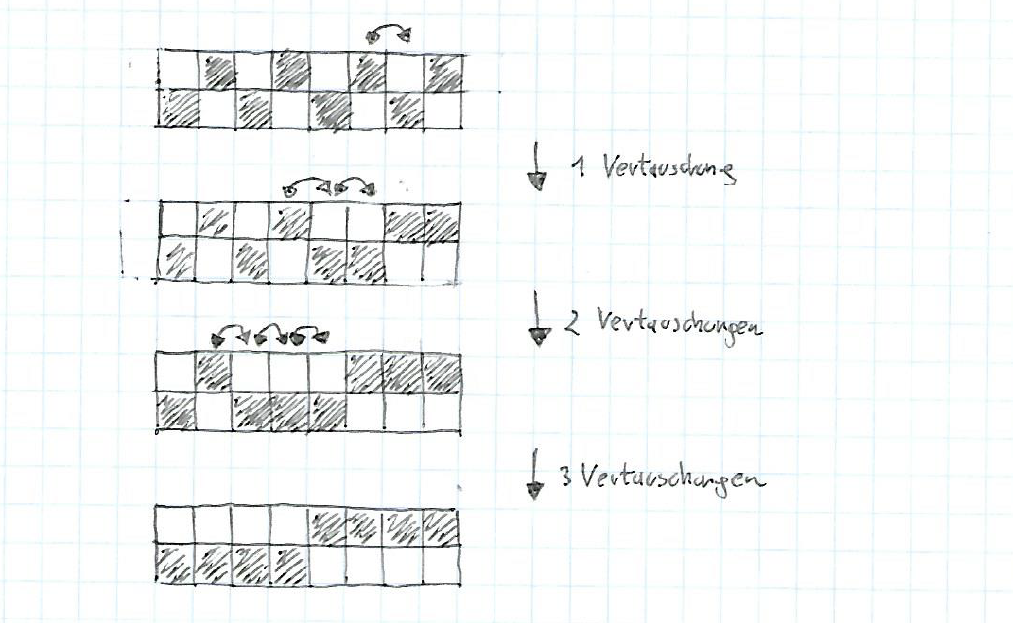
\includegraphics[width = 1\textwidth]{Graphix/Permutation.PNG}
\caption{Veranschaulichung der Permutation $P$ der Zeilen bzw. Spalten von $\bm{M}_I$}
\label{Abb: Permutation für M_I}
\end{figure}


\section{Exakte Berechnung der spontanen Magnetisierung} \label{sec: calcM}
    
Zu Berechnung der spontanen Magnetisierung $\mathcal{M}_S$  wird die Definition \eqref{spontaneMagnetisierung} über die langreichweitige Spin-Spin-Korrelation $l^*$
genutzt.
\begin{equation}
\mathcal{M}_S   = n \mu l^* = n \mu \lim_{m \rightarrow \infty} \sqrt{\corr{\sigma_{0,0}\,\sigma_{m,0}}} 
\end{equation}

\noindent Die benötigte horizontale Spin-Spin-Korrelation lässt sich als Determinante einer komplexen $m+1 \times m+1$ Toeplitz-Matrix schreiben. Mit steigenden $m$ wird die Berechnung zunehmend komplizierter. Zur Berechnung des Grenzwertes der Determinante wird nun die von Elliott W. Montroll, Renfrey B. Potts und John C. Ward verwendete Methode angewandt \cite{Montroll_Potts_Ward}. Dazu wird der starke Szegö Grenzwertsatz benötigt. Eine Formulierung dieses Satzes sei im Folgenden angegeben.    

%\begin{grayframe}[frametitle = {Grenzwertsatz von Szegö}]
%\end{grayframe}


\begin{grayframe}[frametitle = {Starker Grenzwertsatz von Szegö \cite{StrongSzegoeTheorem_Silbermann} }] %\cite{StrongSzegoeTheorem_Hirschman} 
Es sei 
\begin{equation}
f(\omega) = \sum_{k = -\infty}^{\infty} \hat{f}(k)\mathrm{e}^{i k \omega}
\end{equation}
eine Funktion, welche die folgenden Kriterien 
\begin{equation} \label{eq: szego condition}
\sum_{k = -\infty}^{\infty} |\hat{f}(k)| < \infty \;\;\;\text{, }\;\;\;
\sum_{k = -\infty}^{\infty} |\hat{f}(k)|^2 |k| < \infty \\
\end{equation}
erfüllt, die  keine Nullstellen 
\begin{equation}
\forall \omega \in [-\pi,\pi]\;\; :\;\; f(\omega) \neq 0
\end{equation}
auf dem Definitionsintervall besitzt und deren Windungszahl 
\begin{equation}
\left[\mathrm{arg}\left( f\right)\right]_{-\pi}^{\pi} = 0 
\end{equation}
verschwindet. Dann gilt mit
\begin{equation}
D_m(f) = \det{\bm{M}} \;\;\text{ mit}\,\, M_{i,j} = \hat{f}(i-j) 
\end{equation}
dass im Limes $m \rightarrow \infty$ 
\begin{equation}
ln{D_m(f)} = (m+1)\hat{s}(0) + \sum_{k = 1}^{\infty} k \hat{s}(k)\hat{s}(-k) + { \scriptstyle \mathcal{O}}(1)
\end{equation}
gilt, wobei
\begin{equation}
\hat{s}(k) = \frac{1}{2 \pi }  \int_{-\pi}^{\pi} \ln{f(\omega)} \mathrm{e}^{-i k \omega} d \omega 
\end{equation}
\end{grayframe}

\noindent Der starke Szegö Grenzwertsatz liefert damit den Grenzwert einer Folge von Determinaten von Töplitz-Matrizen mit Einträgen $M_{i,j} = \hat{f}(i-j)$, welche sich als Fourier-Koeffizienten einer geeigneten Funktion $f(\omega)$ darstellen lassen. Um diesen Satz für $\det{\bm{C}}$ anwenden zu können, muss also eine geeignete Darstellung der Matrix $\bm{C}$ gefunden werden.

\subsection{Vorbereitung für Szegö-Grenzwertsatz}

Da sich die benötigten Ausdrücke $\corr{h_{l-1,0}^x h_{l',0}^o}$ für die Graßmann-Korrelationen nach dem Übergang in den Thermodynamischen Limes als ein, einem Fourier-Integral ähnlichen, Integral \eqref{eq: corr Integral} schreiben lässt, folgt mit
\begin{equation}
\delta_{l,l+r} = \frac{1}{(2\pi)^2} \int_{-\pi}^{\pi}\int_{-\pi}^{\pi} \d k_1 \d k_2 \mathrm{e}^{i  r k_1}
\end{equation}
und
\begin{equation}
\corr{h^{x}_{(l-1,0)}\, h^{o}_{(l+r, 0)} } = \frac{1}{(2\pi)^2}\int_{-\pi}^{\pi} \int_{-\pi}^{\pi} \d k_1 \d k_2 \,\,\mathrm{e}^{i\, (r+1) \,k_1} \frac{F_{\xi}(k_1,k_2)}{\Delta(k_1, k_2)} 
\end{equation}
aufgrund der Linearität des Integrals, der Ausdruck
\begin{equation}
C_{l,l+r} = \frac{1}{(2\pi)^2} \int_{-\pi}^{\pi}\int_{-\pi}^{\pi} \d k_1 \d k_2 \;\left( t\,\mathrm{e}^{i  r k_1} + (1-t^2) \,\,\mathrm{e}^{i\, (r+1) \,k_1} \frac{F_{\xi}(k_1,k_2)}{\Delta(k_1, k_2)} \right)
\end{equation}
für die Koeffizienten der Matrix $\bm{C}$.
Der Integrand wird auf gleichen Nenner gebracht
\begin{align}
t\mathrm{e}^{i  r k_1} + (1-t^2)\mathrm{e}^{i(r+1)k_1}\frac{F_{\xi}(k_1,k_2)}{\Delta(k_1, k_2)} = \mathrm{e}^{i  r k_1} \frac{t \Delta(k_1, k_2) + (1-t^2) \mathrm{e}^{ik_1} F_{\xi}(k_1,k_2)}{\Delta(k_1, k_2)} \nonumber
\end{align}
und anschließend der Zähler durch Rückeinsetzen explizit berechnet.
\begin{align}
t \Delta(k_1, k_2) + (1-t^2)\mathrm{e}^{ik_1} F_{\xi}(k_1,k_2) &= 2t(1+t^2) - t^2(1-t^2)\mathrm{e}^{-i k_1} - (1-t^2)\mathrm{e}^{i k_1} % =: \tilde{f}(k_1)  \nonumber
\end{align}
Der Zähler hängt nun nicht mehr von $k_2$ ab. Die Integration über $k_2$ kann explizit ausgeführt werden. Mithilfe der Substitutionen \eqref{subs: kappa} bis \eqref{subs: omega} für $\kappa$, $\gamma$ und $\Omega$ ergibt sich
\begin{equation}
\Delta(k_1, k_2) = \Omega - \kappa \cos(k_2)
\end{equation}
Durch Nachrechnen erhält man 
\begin{equation}
 \frac{\gamma}{\kappa} = \frac{(1+t^2)^2}{2t(1-t^2)}> 2 \;\;\;\text{für}\;\;\; t\in \left[0,1\right] 
\end{equation}
und daher  
\begin{equation}
\frac{\kappa}{\Omega} = \frac{\kappa}{\gamma - \kappa \cos(k_1)}  = \frac{1}{\frac{\gamma}{ \kappa} - \cos(k_1)} < 1 
\end{equation}
Mit der Identität 
\begin{equation}
\int_{\pi}^{\pi} \frac{dx}{1 - a\,\cos{x}} = \frac{2\pi}{\sqrt{1 - a^2}} \;\;\;\text{für}\;\;\; |a| < 1 
\end{equation}
ergibt sich das Integral über $k_2$ dann zu
\begin{equation}
\frac{1}{2\pi}\int_{-\pi}^{\pi} \d k_2  \frac{1}{\Delta(k_1, k_2)} = \frac{1}{2\pi}\int_{-\pi}^{\pi} \d k_2  \frac{1}{\Omega - \kappa \cos{k_2}} = \frac{1}{\sqrt{\Omega^2 - \kappa^2}}  
\end{equation}
sodass man insgesamt 
\begin{equation}
C_{l,l+r} = \frac{1}{2\pi} \int_{-\pi}^{\pi} \d k_1  \;\mathrm{e}^{i  r k_1} \frac{2t(1+t^2) - t^2(1-t^2)\mathrm{e}^{-i k_1} - (1-t^2)\mathrm{e}^{i k_1}}{\sqrt{\Omega^2 - \kappa^2}}
\end{equation}
als Darstellung für die Elemente der Matrix $\bm{C}$ erhält. Damit das ganze nun mit der Definition des Fourier-Integrals in Szegös Grenzwertsatz übereinstimmt, wird mit $\omega = -k_1$ substituiert. Insgesamt ergibt sich dann die folgende Darstellung.  

\begin{grayframe}
\begin{equation}
C_{l,l+r} = \frac{1}{2\pi} \int_{-\pi}^{\pi} \d\omega  \;\mathrm{e}^{-i  r \omega} \frac{\tilde{f}(\omega)}{\sqrt{\Omega^2 - \kappa^2}}
\end{equation}
\begin{equation}
\tilde{f}(\omega) = 2t(1+t^2) - t^2(1-t^2)\mathrm{e}^{i \omega} - (1-t^2)\mathrm{e}^{-i \omega}
\end{equation}
\end{grayframe}

\noindent Wie in \cite{Montroll_Potts_Ward} soll nun die Funktion
\begin{equation}
\delta^*(\omega) = \frac{1}{2i} \ln{\frac{(1-tt^*\mathrm{e}^{i\omega})(t-t^*\mathrm{e}^{-i\omega})}{(1-tt^*\mathrm{e}^{-i\omega})(t-t^*\mathrm{e}^{i\omega})}}
\end{equation}
eingeführt werden, wobei 
\begin{equation}
t^* = \frac{(1-t)}{(1+t)}
\end{equation}
gilt.  Die Darstellung der Matrixelemente kann dadurch weiter vereinfacht werden. Im Appendix \ref{Appendix: Nachtrag Rechnung} wird gezeigt dass
\begin{equation} \label{eq: Missing Equation 1}
\mathrm{e}^{2i\delta^*} = \frac{\tilde{f}^{\;2}}{\Omega^2 - \kappa^2}
\end{equation}
gilt. Damit folgt dann 
\begin{equation} \label{eq: f = pm e_i_delta}
\pm \mathrm{e}^{i\delta^*} = \frac{\tilde{f}}{\sqrt{\Omega^2 - \kappa^2}}
\end{equation}
Da für die Spin-Spin-Korrelation im Grenzfall
\begin{equation}
C_{1,1} = \corr{\sigma_{0,0}\, \sigma_{1,0}} \xrightarrow[ T \rightarrow 0 ]{} 1
\end{equation}
gelten muss, wird, da $\delta(\omega) \xrightarrow[ T \rightarrow 0 ]{} 0$ gilt, in \eqref{eq: f = pm e_i_delta} das positive Vorzeichen gewählt. Zusammengefasst erhält man dann das folgende Resultat.

\begin{grayframe}[frametitle = {Darstellung der Matrixelemente $C_{l,l+r}$ als Fourier-Koeffizienten}]
\begin{equation}
C_{l,l+r} = \frac{1}{2\pi} \int_{-\pi}^{\pi}\d\omega  \;\mathrm{e}^{-i  r \omega} \mathrm{e}^{i\delta^*}
\end{equation}
\begin{equation}
i\delta^*(\omega) = \frac{1}{2} \ln{\frac{(1-tt^*\mathrm{e}^{i\omega})(t-t^*\mathrm{e}^{-i\omega})}{(1-tt^*\mathrm{e}^{-i\omega})(t-t^*\mathrm{e}^{i\omega})}}
\end{equation}
\end{grayframe}


\noindent Es folgt
$$i\delta^*(-\omega) = -i\delta^*(\omega)$$
für $\omega \in \left[-\pi,\pi\right]$ und $i\delta^*(-\pi) =  i\delta^*(\pi) = 0$, da $\mathrm{e}^{-i \pi} = -1 = \mathrm{e}^{i \pi}$ gilt. 
Zudem ist $ i\delta^* $ als Logarithmuss einer rationalen Funktion ohne Polstellen auf dem Einheitskreis eine holomorphe Funktion in $z= \mathrm{e}^{i\omega}$ für alle $t \in (0,1)$. Daher ist $i\delta^*$ zumindest 2 mal stetig differenzierbar in $\omega \in \left[-\pi,\pi\right]$.  Somit existiert die Fourier-Reihe von $\mathrm{e}^{i\delta^*}$. Diese konvergiert zudem dann gleichmäßig gegen die Funktion und die Reihe selbst konvergiert normal (d.h. wie in \eqref{eq: szego condition} gefordert). Zudem konvergiert die, durch gliedweise Differentiation erhaltene, Reihe auch normal, wodurch sich
\begin{equation}
 \sum_{k = -\infty}^{\infty} |\hat{f}(k)|^2|k| < \sum_{k = -\infty}^{\infty} |\hat{f}(k)|^2|k|^2 < \left(\sum_{k = -\infty}^{\infty} |\hat{f}(k)||k|\right)^2 < \infty
\end{equation}
ergibt. Die Funktion $\mathrm{e}^{i\delta^*}$ erfüllt daher alle Vorraussetzungen des starken Grenzwertsatzes von Szegö.

\subsection{Die kritische Temperatur $T_C$}

Um nun den Satz von Szegö zu benutzen müssen die Größen  $\hat{s}(k)$ berechnet werden.
Da $f = \mathrm{e}^{i\delta^*}$ gilt, folgt $\ln{f)} = i \delta^*$ und daher
\begin{equation}
\hat{s}(0) = \frac{1}{2\pi} \int_{-\pi}^{\pi} \d\omega\; i \delta^*(\omega)  = 0
\end{equation}
da $i \delta^*$ eine ungerade Funktion in $\omega$ ist. Zur Berechnung der Fourier-Koeffizienten von $\ln{f}$ wird $i\delta^*$,  wie in \cite{Montroll_Potts_Ward}, mithilfe der Reihendarstellung des Logarithmus in eine Laurent-Reihe entwickelt.
\begin{equation} \label{eq: idelta = frac} 
i\delta^* = \frac{1}{2} \ln{\frac{(1-tt^*\mathrm{e}^{i\omega})(1-\frac{t^*}{t}\mathrm{e}^{-i\omega})}{(1-tt^*\mathrm{e}^{-i\omega})(1-\frac{t^*}{t}^*\mathrm{e}^{i\omega})}}
\end{equation}
Um die Reihen-Darstellung des Logarithmus verwenden zu können, muss jedoch sowohl $tt^* < 1$ als auch $t^* < t $ gelten. Während erstere Bedingung immer erfüllt ist, führt die zweite Bedingung auf die Ungleichung
\begin{equation}
(1-t) < (1+t)t  
\end{equation}
bzw. durch umformen
\begin{equation}
\sqrt{2}-1 < t
\end{equation}
für den Parameter $t$. Über die Definiton des Parameters $t = \tanh(\frac{J}{k_B T})$ ergibt sich dann 
\begin{equation} \label{eq: umformun condition krit temp}
\frac{J}{k_B T} > \mathrm{atanh}\left(\sqrt{2}-1\right) = \frac{1}{2} \ln{\frac{1+(\sqrt{2}-1)}{1+(\sqrt{2}-1)}} = \frac{1}{2} \ln{1+\sqrt{2}}
\end{equation}
als Bedingung für die Temperatur. Dadurch lässt sich eine kritische Temperatur $T_c$ für das System definieren.
\begin{grayframe}[frametitle = {Kritische Temperatur $T_C$}]
\begin{equation}
T_C  := \frac{2 J}{ \ln{1+\sqrt{2}} k_B}
\end{equation}
\end{grayframe}

\subsection{Magnetisierung für $T < T_C$}

Für den Fall $T < T_C$ gilt
$$ t^* < t$$
und es lässt sich die vorherige Darstellung \eqref{eq: idelta = frac} für $i\delta^*$ verwenden. 
Hier wird analog zu \cite{Montroll_Potts_Ward} vorgegangen. Durch Anwendung der Rechenregeln für den Logarithmus erhält man dann
\begin{equation} \nonumber
i\delta^* = \frac{1}{2} \left(\ln{1-tt^*\mathrm{e}^{i\omega}} + \ln{1-\frac{t^*}{t}\mathrm{e}^{-i\omega}} - \ln{(1-tt^*\mathrm{e}^{-i\omega}} - \ln{1-\frac{t^*}{t}^*\mathrm{e}^{i\omega}} \right)
\end{equation}
und mithilfe der Reihendarstellung
\begin{equation} \nonumber 
\ln{1-x} = \sum_{k=1}^{\infty} -\frac{x^k}{k}
\end{equation}
ergibt sich dann 
\begin{align} \nonumber
i\delta^* &= \frac{1}{2} \left(  \sum_{k=1}^{\infty} -\frac{(tt^*)^k}{k}\mathrm{e}^{i k \omega} - \frac{(t^*)^k}{t^kk}\mathrm{e}^{-i k \omega} + \frac{(tt^*)^k}{k}\mathrm{e}^{-i k \omega} + \frac{(t^*)^k}{t^kk}\mathrm{e}^{i k \omega}\right) \nonumber \\
          &= \left(  \sum_{k=1}^{\infty} \left(\frac{(t^*)^k}{t^k}-(tt^*)^k\right)\frac{1}{2 k}\mathrm{e}^{i k \omega} + \left((tt^*)^k - \frac{(t^*)^k}{t^k}\right)\frac{1}{2 k}\mathrm{e}^{-i k \omega} \right)
\end{align}
Aus dieser Darstellung lässt sich
\begin{equation}  \nonumber
\hat{s}(k) = - \hat{s}(-k) = \frac{1}{2 k} \left((\frac{(t^*)^k}{t^k} - tt^*)^k\right)
\end{equation}
für die Fourier-Koeffizienten der Funktion $\ln{f}$ ablesen. Damit folgt
\begin{equation}  
\hat{s}(k)\hat{s}(-k) =  -\frac{1}{4k}\left(\frac{(( tt^*)^2)^k}{k} + \left(\frac{(t^*)^{2}}{t^{2}}\right)^k \frac{1}{k}- 2\frac{((t^*)^2)^k}{k}\right)
\end{equation}
und somit 
\begin{align} 
% \sum_{k=1}^{\infty} \hat{s}(k)\hat{s}(-k)k
\sum_{k = 1}^n k \hat{s}(k)\hat{s}(-k) &= -\frac{1}{4} \sum_{k=1}^{\infty}  \left(\frac{(( tt^*)^2)^k}{k} + \left(\frac{(t^*)^{2}}{t^{2}}\right)^k \frac{1}{k}- 2\frac{((t^*)^2)^k}{k}\right) \nonumber \\
&= \frac{1}{4} \left(\ln{1-(tt^*)^2} + \ln{1-\frac{(t^*)^{2}}{t^{2}}} - 2\ln{1-(t^*)^2} \right) \nonumber \\
&= \ln{\left(\frac{(1-(tt^*)^2)(1-\frac{(t^*)^{2}}{t^{2}})}{(1-(t^*)^2)^2}\right)^{\frac{1}{4}}}  \nonumber
\end{align}
Durch Rücksubstitution und Umformung folgt 
\begin{equation} \label{eq: Missing Equation 2}
\ln{\left(\frac{(1-(tt^*)^2)(1-\frac{(t^*)^{2}}{t^{2}})}{(1-(t^*)^2)^2}\right)^{\frac{1}{4}}} = \frac{1}{4} \ln{1 - \frac{(1-t^2)^4}{16t^4}}
\end{equation}
wie in Appendix \ref{Appendix: Nachtrag Rechnung} ausführlich bewiesen wird. Für den Grenzübergang mit $D_m = \det{\bm{C}^{I_m I_m}}$ folgt dann aufgrund des starken Szegö Grenzwertsatzes
\begin{align}  \nonumber
 \lim_{m \rightarrow \infty} \ln{D_m} & = \frac{1}{4} \ln{1 - \frac{(1-t^2)^4}{16t^4}}
 \end{align}
Dabei wurde $\hat{s}(0)= 0$ verwendet. Für die spontane Magnetisierung ergibt sich letztlich   
\begin{align} \nonumber
\frac{\mathcal{M}_S}{n\mu} =  \lim_{m \rightarrow \infty} \sqrt{D_m} =  \left(1 - \frac{(1-t^2)^4}{16t^4}\right)^{\frac{1}{8}}
 \end{align}
Als letztes erfolgt die Rücksubstitution des Systemparameters $t=\tanh(\frac{J}{k_B T})$. 
\begin{align} \nonumber
\frac{1-t^2}{16t^4} = \frac{1}{\sinh(\frac{J}{k_B T})^4 \cosh(\frac{J}{k_B T})^4} = \frac{1}{\sinh(\frac{2J}{k_B T})^4} 
 \end{align}
\begin{grayframe}[frametitle = {Spontane Magnetisierung für $T < T_C$}]
\begin{equation} \label{eq: result magnetisation low}
\mathcal{M}_S = n\mu\left(1-\frac{1}{\sinh(\frac{2J}{k_B\,T})^4}\right)^{\frac{1}{8}}
\end{equation}
\end{grayframe}

\subsection{Magnetisierung für $T > T_C$}

Für den Fall $T > T_C$ gilt
$$ t^* > t$$
und der Ausdruck \eqref{eq: idelta = frac} für $i\delta^*$ muss, wie in \cite{Montroll_Potts_Ward}, anders umgeformt werden, um die Reihen-Darstellung des Logarithmus nutzen zu können. In der Form
\begin{align}
i \delta^* &= \frac{1}{2} \ln{ \frac{(1-tt^*\mathrm{e}^{i\omega})(1-\frac{t}{t^*}\mathrm{e}^{-i\omega})}                                  {(1-tt^*\mathrm{e}^{-i\omega})(1-\frac{t}{t^*}\mathrm{e}^{i\omega})}\mathrm{e}^{-2i\omega} } \nonumber 
\end{align}
kann der Logarithmus auch in der Variable $t/t^*$ in eine Taylorreihe entwickelt werden.
Durch anwenden der Rechenregeln und Reihen-Darstellung des Logarithmus erhält man
\begin{align}
i \delta^* &= \frac{1}{2}\left( \sum_{k = 1}^{\infty} - \frac{(tt^*)^k}{k}\mathrm{e}^{i\omega k} - \frac{1}{k}\frac{(t)^k}{(t^*)^k}\mathrm{e}^{-i\omega k} + \frac{(tt^*)^k}{k}\mathrm{e}^{-i\omega k} + \frac{1}{k}\frac{(t)^k}{(t^*)^k}\mathrm{e}^{i\omega k}\right) -i\omega  \nonumber 
\end{align}
Die Gerade $i\omega$ wird am Einheitskreis als imaginäre Sägezahn-Funktion  periodisch fortgesetzt. Die Fourierkoeffizienten
\begin{equation} \nonumber
\frac{1}{2 \pi } \int_{- \pi}^{\pi}\d\omega \; i\omega \mathrm{e}^{-i k \omega} = \frac{\cos(k \pi)}{k}  = \frac{(-1)^k}{k}
\end{equation}
ergeben sich leicht durch partielle Integration. Zusammengefasst in der Darstellung
\begin{align} \nonumber
i \delta^* &= \sum_{k = 1}^{\infty} \frac{1}{2k} \left(  \left(\frac{(t)}{(t^*)}\right)^k - (tt^*)^k + 2(-1)^k  \right)\mathrm{e}^{i\omega k} +  \frac{1}{2k} \left(  \left((tt^*)^k - \frac{(t)}{(t^*)}\right)^k - 2(-1)^k \right)  \mathrm{e}^{-i\omega k}
 \nonumber 
\end{align}
erkennt man dass
\begin{align} \nonumber
\hat{s}(k) = - \hat{s}(-k) = \frac{1}{2k} \left(  \left(\frac{(t)}{(t*)}\right)^k - (tt*)^k + 2(-1)^k  \right)
\end{align} 
für die Fourier-Koeffizienten der Funktion $\ln{f} = i\delta^*$ gilt. Damit folgt
\begin{align} \nonumber
\hat{s}(k)\hat{s}(-k)k = -\frac{1}{k} - \frac{1}{4k} \left(  \left(\frac{(t)}{(t*)}\right)^k - (tt*)^k\right)^2 - (-1)^n  \left(  \left(\frac{(t)}{(t*)}\right)^k - (tt*)^k\right)
\end{align}
und somit gilt für den Grenzübergang
\begin{align} \nonumber
 \lim_{m \rightarrow \infty} \ln{D_m} & = \lim_{m \rightarrow \infty} \sum_{k = 1}^{m} \hat{s}(k)\hat{s}(-k)k = -\infty 
\end{align}
da die harmonische Reihe immer divergiert. Somit verschwindet die Magnetisierung für $T > T_C$

\begin{grayframe}[frametitle = {Spontane Magnetisierung für $T < T_C$}]
\begin{equation} \label{eq: result magnetisation high}
\mathcal{M}_S = n\mu\ \lim_{m \rightarrow \infty} D_m = 0
\end{equation}
\end{grayframe}


\section{Zusammenfassung und Fazit} \label{sec: conclusion} \label{sec: conclusio}
    
Die Ergebnisse \eqref{eq: result magnetisation low} und \eqref{eq: result magnetisation high} für die Magnetisierung unterhalb und oberhalb der kritischen Temperatur $T_C$ ergeben zusammengefasst die, erstmals von Lars Onsager aufgestellte, Formel für die spontanen Magnetisierung in Abhängigkeit der Temperatur.

\begin{grayframe}[frametitle = {Spontane Magnetisierung des 2d Ising-Modells}]
\begin{equation} \label{eq: result Magnetisation}
\mathcal{M}_S = \left\{ \begin{array}{cr} n \mu \left(1-\frac{1}{\sinh(\frac{2J}{k_B\,T})^4}\right)^{\frac{1}{8}} & \text{für } T < T_c \\ 0 &\text{für } T > T_c   \end{array} \right.
\end{equation}
\begin{equation} 
T_C  := \frac{2 J}{ \ln{1+\sqrt{2}} k_B}
\end{equation}
\end{grayframe}

\noindent Der Beweis ist damit abgeschlossen. Nebenbei wurde zudem ein Ausdruck für die Zustandssumme abgeleitet, der eine leichte, explizite Berechnung dieser und der Freien Energie des Modells ermöglicht. Dies wird in Appendix \ref{Appendix: Zustandsumme} vorgeführt.\\

\noindent Der Ansatz das Problem der Zählung geschlossener Graphen auf dem rechteckigen Gitter, mithilfe einer graphischen Überlegung, in ein algebraisches Problem für Graßmann Zahlen zu übersetzen, bietet nicht nur einen anschaulichen Zugang, sondern ermöglicht die Anwendung leicht handhabbarer algebraischer Methoden und Hilfsmittel. Zudem gelingt es mit diesem Ansatz nicht nur die Zustandsumme, sondern auch die Magnetisierung mit absehbarem Aufwand zu berechnen. 
% Der Erfolg des Ansatzes beruht dabei darauf die physikalische Größen, wie die Zustandssumme oder Spinn-Spin-Korrelationen, welche eine physikalische Interpretation besitzen aber mathemathisch schwer handhabbar sind, mit leichter zugänglichen mathemathischen Hilfsgrößen, wie dem Spurintegral einer geeigneten Graßmann-Dichte und Korreltationen geeigneter Graßmann-Funktionen, in Verbindung zu bringen. 
\\
Aus Sicht der Quantenfeldtheorie wurde das Problem mithilfe der Graßmann Variablen in ein Freies Fermionen Modell übersetzt, das dann mit den, in der QFT üblichen Methoden, behandelt werden kann. Dies war auch Stuart Samuels ursprünglicher Zugang. Dieser Ansatz ist zudem nicht nur auf das Ising-Modell beschränkt, sondern kann auch zu exakten Lösung andere Probleme wie ``planar closed-Packed Dimer Problems'' genutzt werden \cite{StuartSamuel1} \cite{StuartSamuel2}. \\ 
Der starke Grenzwertsatz von Szegö erweist sich als mächtiges Hilfsmittel wenn es um die Berechnung von Grenzwerten von Folgen von Töplitz-Determinanten geht. Töplitz-Matrizen stehen dabei in einem natürlichen Zusammenhang mit den in der Physik häufig auftretenden periodischen Randbedingungen. Die Notwendigkeit des Übergangs in ein unendlich großes System, um physikalische Aussagen treffen zu können, stellt dabei eine häufige Schwierigkeit dar.\\

\noindent Die erbrachte Herleitung weist jedoch einen Mangel auf, welche den hier gelieferten Beweis aus mathematischer Sicht unvollständig macht. Dies wurde in Abschnitt \ref{sec: Wahl der übrigen Koeffizienten} bereits angesprochen und in Appendix \ref{Appendix: Zustandsumme} genauer ausgeführt. Im Temperaturbereich $T < T_C$ hat der, über die Hochtemperatur-Darstellung hergeleitete, Ausdruck für die Zustandssumme zwar den richtigen Absolutbetrag aber das falsche Vorzeichen. Am kritischen Punkt für $T = T_C$ wechselt der berechnete Ausdruck für die Zustandssumme das Vorzeichen. Der Vorzeichenwechsel geht dabei stetig von statten. Eine negative Zustandssumme ist jedoch weder aus mathematischer, noch physikalischer Sicht, sinnvoll, sodass sich hier um einen Fehler handeln muss. Tatsächlich scheint es, als würde es am kritischen Punkt zu einer Art Perkolations-Phänomen kommen, das dafür sorgt, dass die Beiträge der, in Abschnitt \ref{sec: Wahl der übrigen Koeffizienten} eingeführten, äußere Graphen nicht mehr im Thermodynamischen Limes verschwinden. Denn diese wurden als einzige mit negativer Gewichtung gezählt. Konkret fehlt es hier an einer qualitativen Abschätzung für die Geschwindigkeit mit der die Beiträge dieser äußeren Graphen verschwinden und einer Abschätzung des Temperaturbereiches in dem diese tatsächlich verschwinden. Dem Autor sind bislang keine Arbeiten bekannt, die diese Themen behandeln würden und auch in anderen Herleitungen, welche die hier verwendeten Methoden zur Lösung des Ising-Modells benutzen, wie \cite{PostBac} \cite{Gandhi}, oder in den ursprunglichen Arbeiten von Stuart Samuel \cite{StuartSamuel1} \cite{StuartSamuel2}, wird dieses Detail nicht erwähnt. \\
Für die Berechnung der spontanen Magnetisierung scheint dieses Verhalten jedoch keinen Unterschied zu machen, da diese als Quotient zweier Zustandssummen ausgedrückt werden kann und das Vorzeichen somit keine Rolle spielt. Zudem kann mit den hier besprochenen Methoden auch ein für $T < T_C$ gültiger Ausdruck für die Zustandssumme unter Hinzunahme der sogenannten Tieftemperatur-Darstellung abgeleitet werden. Dies wird ebenfalls in Appendix \ref{Appendix: Zustandsumme} gezeigt und stellt keinen wirklichen Mehraufwand dar. 



\newpage 

%%%%%%%%%%%%%%%%%%%%%%%%%%%%%%%%%%%%%%%%%%%%%%%%%%%%%%%%%%%%%%%%%%%%%%%%%%%%%%%
\appendix

\section{Appendix: Explizite Berechnung der Zustandssumme}
    \label{Appendix: Zustandsumme}
    \input{Appendix/Zustandssumme.tex}
    \newpage 
\section{Appendix: Beweise der Eigenschaften Pfaffscher Determinanten mithilfe von Graßmann-Variablen}
    \label{Appendix: Pfaffians with GV}
    \input{Appendix/Pfaffian_Beweise.tex}
    \newpage 
\section{Appendix: Permutationen}
    \label{Apenndix: Permutationen}
    \input{Appendix/Permutationen.tex}
    \newpage 
\section{Appendix: Fouriermatrix auf 2d Gitter }
    \label{Appendix: Det Fouerier}
    \input{Appendix/Fouriermatrix2D.tex}
    \newpage 
\section{Appendix: Satz über Koeffizienten des charakteristischen Polynoms }
    \label{appendix: Satz über Koeffizienten des Charakteristischen Polynoms}
    \input{Appendix/Satz_ueber_charakteristisches_polynom.tex}
    \newpage 
\section{Appendix: Nachtrag der verschobenen Rechnungen aus Kapitel \ref{sec: calcM} }
    \label{Appendix: Nachtrag Rechnung}
    \input{Appendix/Nachtrag_Rechnungen.tex}
    \newpage 

    
    

%\section{Appendix: On the strong Szego limit theorem}
%%%%%%%%%%%%%%%%%%%%%%%%%%%%%%%%%%%%%%%%%%%%%%%%%%%%%%%%%%%%%%%%%%%%%%%%%%%%%%%
%Literaturverzeichnis etc. 
\newpage
% \listoffigures
% \listoftables

\bibliographystyle{Literature/seminarstyle}
\bibliography{Literature/Literature}

\end{document}
%%%%%%%%%%%%%%%%%%%%%%%%%%%%%%%%%%%%%%%%%%%%%%%%%%%%%%%%%%%%%%%%%%%%%%%%%%%%%%%
%%%%%%%%%%%%%%%%%%%%%%%%%%%%%%%%%%%%%%%%%%%%%%%%%%%%%%%%%%%%%%%%%%%%%%%%%%%%%%%




